% Template for DAN, KLTN, SVNCKH 

\documentclass[oneside,a4paper,13pt]{extreport}

% --- PHẦN PREAMBLE (CÁC GÓI LỆNH) ---
% --- Cấu hình tiếng Việt cho nhãn hình, bảng, phụ lục ---
\usepackage[vietnamese]{babel}
\addto\captionsvietnamese{
	\renewcommand{\figurename}{Hình}
	\renewcommand{\tablename}{Bảng}
	\renewcommand{\appendixname}{Phụ lục}
}
\usepackage[T5]{fontenc}
\usepackage[utf8]{inputenc}
\DeclareTextSymbolDefault{\DH}{T1}

% Tài liệu tham khảo
\usepackage[backend=biber, style=numeric, sorting=none, giveninits=true]{biblatex}
\addbibresource{References/references.bib}

% Chèn hình
\usepackage{graphicx}
\graphicspath{ {images/} }

% Chèn và định dạng mã nguồn (listings)
\usepackage{listings}
\usepackage{color}
% ... (Giữ nguyên các định dạng màu sắc của bạn)

% Chèn và định dạng mã giả, bảng biểu, tiêu đề...
\usepackage{amsmath}
\usepackage{algorithm}
\usepackage[noend]{algpseudocode}
\usepackage{titlesec}
\usepackage{setspace}
\usepackage{indentfirst}
\usepackage{geometry}
\usepackage{tikz}
\usetikzlibrary{calc}      
\usepackage[hidelinks]{hyperref}

% --- SỬA LỖI TẠI ĐÂY ---
% 1. Lệnh \includeonly PHẢI nằm ở đây (trước \begin{document}).
% 2. Chỉ dùng MỘT lệnh duy nhất, liệt kê các chương cách nhau bằng dấu phẩy.
% 3. Muốn biên dịch chương nào thì để tên chương đó, muốn ẩn thì xóa hoặc comment.

% \includeonly{Chapter1/chapter1,Chapter2/chapter2,Chapter3/chapter3} 
% \includeonly{Chapter1/chapter1,Chapter2/chapter2}

% --- HẾT PHẦN PREAMBLE ---


\begin{document}

\begin{titlepage}
\begin{center}

BỘ GIÁO DỤC VÀ ĐÀO TẠO\\
{TRƯỜNG ĐẠI HỌC MỞ THÀNH PHỐ HỒ CHÍ MINH}\\[1.cm]


\includegraphics[scale=0.15]{images/logo}\\[1.cm]

{\large \bfseries TRẦN VĂN NHANH - 2251052079\\[2cm]}

%Tên đề tài Khóa luận tốt nghiệp/Đồ án ngành
{ \huge \bfseries  Phát triển hệ thống hỗ trợ học từ vựng tiếng Anh sử dụng ASP.NET Core và ReactJS kết hợp gamification
\\[2cm] } 


%Chọn một trong các dòng sau
\large KHÓA LUẬN TỐT NGHIỆP\\

%Chọn một trong các dòng sau
\large NGÀNH CÔNG NGHỆ THÔNG TIN\\[2cm]
%\large NGÀNH KHOA HỌC MÁY TÍNH\\[2cm]
%\large NGÀNH HỆ THỐNG THÔNG TIN QUẢN LÝ\\[2cm]
%\large NGÀNH TRÍ TUỆ NHÂN TẠO\\[2cm]


Giảng viên hướng dẫn:\\
\textbf{ThS. NGUYỄN TRUNG HẬU}


\begin{tikzpicture}[remember picture, overlay]
  \draw[line width = 2pt] ($(current page.north west) + (1.5cm,-2cm)$) rectangle ($(current page.south east) + (-1.5cm,3cm)$);
\end{tikzpicture}

\vfill
TP. Hồ Chí Minh, 2026

\end{center}

\end{titlepage}
\pagenumbering{roman}


% ... (Các phần Ý kiến GV giữ nguyên)
\chapter*{Lời cảm ơn}
\addcontentsline{toc}{chapter}{Lời cảm ơn}

Khóa luận tốt nghiệp là cột mốc đánh dấu sự kết thúc của một hành trình học thuật dài, nơi sự kiên trì của cá nhân được nuôi dưỡng bởi sự chỉ dẫn và khích lệ từ những người đồng hành đáng quý. Tôi nhận thức rằng nếu không có những điểm tựa vững chắc ấy, công trình này khó có thể hình thành một cách trọn vẹn.

Lòng biết ơn chân thành nhất xin được dành cho ThS. Nguyễn Trung Hậu, người đã trực tiếp dẫn dắt đề tài. Những rào cản kỹ thuật khi vận hành các công nghệ hiện đại như ReactJS hay hệ sinh thái .NET 8 đã không còn là trở ngại nhờ sự định hướng tận tâm và những lời khuyên chuyên môn sắc sảo từ Thầy. Hơn cả kiến thức chuyên ngành, phong cách làm việc kỷ luật và tư duy phản biện khoa học mà Thầy truyền thụ chính là hành trang quý báu nhất trên con đường nghiên cứu và phát triển nghề nghiệp.

Bốn năm học tập dưới mái trường Đại học Mở Thành phố Hồ Chí Minh là khoảng thời gian để tôi được trau dồi những nền tảng tri thức quan trọng nhất. Xin trân trọng cảm ơn Ban Giám hiệu cùng tập thể sư phạm Khoa Công nghệ Thông tin đã kiến tạo một môi trường giáo dục chất lượng, tạo điều kiện để tôi có đủ nền tảng kỹ thuật nhằm chuyển đổi những ý tưởng trên bản vẽ thành một hệ thống có tính ứng dụng thực tiễn.

Gia đình chính là nguồn động lực bền vững và là chỗ dựa tinh thần vững chắc nhất trong suốt quá trình học tập và nghiên cứu. Niềm tin và sự cổ vũ không điều kiện từ người thân đã tiếp thêm ý chí để tôi theo đuổi và hoàn thành tốt đề tài này.

Xin gửi lời cảm ơn đến các bạn bè và anh chị đồng nghiệp đã đồng hành trong suốt quá trình thực hiện. Những cuộc trao đổi cởi mở và các góp ý thực tế từ mọi người là những mảnh ghép quan trọng giúp dự án khắc phục nhiều hạn chế và trở nên hoàn thiện hơn.

Mặc dù đã đầu tư nhiều tâm huyết và sự cẩn trọng, khóa luận này chắc chắn vẫn còn những khía cạnh có thể phát triển thêm. Tôi trân trọng mọi ý kiến phản biện từ Hội đồng và quý Thầy Cô, bởi đó là cơ hội quý giá để nhìn nhận lại sản phẩm và nâng cao giá trị ứng dụng của đề tài trong tương lai.\\

\noindent Xin trân trọng cảm ơn!

\tableofcontents

\listoffigures

\clearpage
\pagenumbering{arabic} 

% --- THAY ĐỔI CÁCH GỌI CHƯƠNG ---
% Sử dụng \include thay vì \includeonly ở đây. 
% LaTeX sẽ đối chiếu danh sách trong \includeonly ở trên để quyết định có nạp file này hay không.

\chapter{Giới thiệu}
\label{Chapter1}

\section{Lý do chọn đề tài}

Trong bối cảnh toàn cầu hóa hiện nay, năng lực sử dụng tiếng Anh đã trở thành một trong những tiêu chuẩn bắt buộc cho mọi hoạt động học tập và phát triển nghề nghiệp. Nền tảng của sự thông thạo ngôn ngữ này nằm ở việc xây dựng và duy trì một vốn từ vựng phong phú, bởi đây là yếu tố then chốt chi phối trực tiếp đến hiệu quả của cả bốn kỹ năng nghe, nói, đọc và viết \cite{Nation2001}. Tuy nhiên, thực trạng hiện nay cho thấy người học thường đối mặt với thách thức lớn trong việc chuyển dịch thông tin từ trí nhớ ngắn hạn sang dài hạn, dẫn đến sự đứt gãy trong lộ trình học tập do hiện tượng quên lãng tự nhiên.

Mặc dù các cơ sở khoa học về nhận thức như kỹ thuật lặp lại có khoảng cách (Spaced Repetition) và thực hành truy hồi (Retrieval Practice) đã chứng minh được hiệu quả vượt trội trong việc củng cố dấu vết trí nhớ \cite{Cepeda2008, Karpicke2008}, nhưng thực tế triển khai trên các nền tảng học ngôn ngữ phổ biến vẫn bộc lộ một khoảng trống quan trọng hơn: vấn đề duy trì động lực học tập dài hạn. Người học không bỏ cuộc vì thiếu phương pháp — họ bỏ cuộc vì quá trình lặp lại từ vựng ngày qua ngày trở nên đơn điệu, nhàm chán và thiếu cơ chế phản hồi đủ để duy trì động lực học tập trong dài hạn.

Anki cung cấp thuật toán lặp lại ngắt quãng chính xác nhưng giao diện tối giản và thiếu phản hồi tích cực. Người học dễ rơi vào trạng thái học cơ học thụ động — lật thẻ, đánh giá, lật thẻ tiếp — mà không nhận thấy sự tiến bộ hay gắn kết với nội dung, dẫn đến giảm động lực sau vài tuần đầu. Duolingo ở chiều ngược lại, cố gắng bù đắp bằng hệ thống động lực ngoại tại (Extrinsic Motivation): chuỗi ngày liên tục (streak), bảng xếp hạng điểm số, phần thưởng ảo. Song theo Thuyết Tự Quyết (Self-Determination Theory), các cơ chế ngoại tại này không nuôi dưỡng được hai yếu tố cốt lõi của động lực bền vững là cảm giác năng lực (Competence) và tính tự chủ (Autonomy). Khi streak bị gián đoạn hoặc khi phần thưởng ngoại tại mất đi sức hấp dẫn, toàn bộ động lực học tập sụp đổ theo, để lại người học không có lý do nội tại nào để tiếp tục.

Nhằm giải quyết những tồn tại này, khóa luận đã thực hiện đề tài \textbf{"Phát triển hệ thống hỗ trợ học từ vựng tiếng Anh sử dụng ASP.NET Core và ReactJS kết hợp gamification"}. Đề tài được lựa chọn dựa trên ba trụ cột mục tiêu chiến lược: 
(1) Hiện thực hóa quy trình ghi nhớ dựa trên thuật toán SM-2 tiêu chuẩn, bổ sung hàm chấm điểm đa yếu tố tự động (\texttt{CalculateSm2Grade}) để thay thế bước tự đánh giá thủ công trong SM-2 gốc bằng tính toán dựa trên độ chính xác, tốc độ phản hồi và số gợi ý sử dụng; 
(2) Xây dựng cơ chế gắn kết học tập thông qua hệ thống thú ảo gắn liền với tiến trình học tập; 
(3) Hiện thực hóa giải pháp trên một nền tảng kỹ thuật vững chắc theo kiến trúc hành tây (Onion Architecture) với hệ sinh thái .NET 8 và ReactJS để đảm bảo tính mở rộng và khả năng bảo trì cao.

\section{Mục tiêu đề tài}
Mục tiêu của đề tài là nghiên cứu và xây dựng một nền tảng học từ vựng trực tuyến, nhằm giải quyết hai thách thức trong việc tiếp thu ngôn ngữ: hiệu suất ghi nhớ dài hạn và khả năng duy trì động lực học tập. Để đạt được điều này, hệ thống hiện thực hóa thuật toán lặp lại ngắt quãng SuperMemo-2 (SM-2), một mô hình toán học tiên tiến cho phép cá nhân hóa hoàn toàn lộ trình ôn tập dựa trên khả năng phản hồi thực tế của từng cá nhân. Việc ứng dụng thuật toán này giúp tối ưu hóa "thời điểm vàng" để truy hồi kiến thức, từ đó hỗ trợ người học chuyển dịch thông tin từ trí nhớ ngắn hạn sang trí nhớ dài hạn một cách hiệu quả nhất.

Bên cạnh giải pháp về mặt kỹ thuật nhận thức, đề tài còn tập trung nghiên cứu sự giao thoa giữa tâm lý học hành vi và phát triển phần mềm thông qua việc tích hợp các cơ chế trò chơi hóa (Gamification) chuyên sâu. Hệ thống không chỉ dừng lại ở các yếu tố bề nổi mà còn xây dựng một cấu trúc tương tác phức hợp, tiêu biểu là cơ chế nuôi dưỡng và tiến hóa thú ảo. Phương pháp tiếp cận này nhằm tăng tính tương tác trong quá trình học tập, qua đó đáp ứng các nhu cầu tâm lý về sự tự chủ (Autonomy) và năng lực (Competence) theo Thuyết Tự Quyết (Self-Determination Theory). Sự kết hợp giữa cơ sở khoa học nhận thức và cơ chế trò chơi hóa được kỳ vọng hỗ trợ người học duy trì thói quen ôn tập từ vựng hiệu quả hơn.

\section{Phạm vi đề tài}

Đề tài tập trung vào việc nghiên cứu và xây dựng một ứng dụng web (Web Application) có khả năng vận hành đa nền tảng, hướng tới đối tượng mục tiêu là người học tiếng Anh ở trình độ từ cơ bản đến trung cấp. Phạm vi của nghiên cứu được xác định cụ thể thông qua sự kết hợp giữa các tính năng nghiệp vụ sư phạm và các tiêu chuẩn kỹ thuật phần mềm hiện đại.

Về mặt chức năng, hệ thống ưu tiên thiết lập các công cụ quản lý bộ từ vựng cá nhân hóa, cho phép người học chủ động trong việc xây dựng kho học liệu riêng. Quy trình học tập được hiện thực hóa thông qua bốn dạng tương tác cốt lõi bao gồm: Flashcard, Fill-in-blank (điền vào chỗ trống), Multiple Choice (trắc nghiệm) và Listening (nghe hiểu). Các phương thức này được thiết kế để bao quát các khía cạnh của trí nhớ ngôn ngữ từ nhận diện đến truy hồi kiến thức. Bên cạnh đó, đề tài chú trọng triển khai hệ thống quản lý thú ảo như một cơ chế trò chơi hóa chuyên sâu, đóng vai trò then chốt trong việc duy trì động lực và sự gắn kết của người học với nền tảng.

Về phương diện kỹ thuật, đề tài tập trung vào việc thiết kế và hiện thực hóa hệ thống theo kiến trúc hành tây (Onion Architecture), hay còn gọi là Clean Architecture. Việc áp dụng mô hình kiến trúc này nhằm đảm bảo sự tách biệt giữa logic nghiệp vụ (Business Logic) và tầng hạ tầng kỹ thuật (Infrastructure), từ đó cải thiện khả năng kiểm thử, bảo trì và tính độc lập giữa các lớp.

Cần lưu ý rằng hệ thống bao gồm nhiều tính năng (thú ảo, PvP/PvE, nhiệm vụ, thành tích, quản trị) vì các tính năng này được thiết kế như một hệ thống Gamification tích hợp, trong đó đóng góp kỹ thuật cốt lõi là hiện thực hóa thuật toán SM-2 và cơ chế ghi nhớ đa dạng; các tính năng Gamification đóng vai trò là phương tiện duy trì động lực học tập, không phải là mục tiêu nghiên cứu độc lập. Ngoài phạm vi trên, đề tài không bao gồm việc giảng dạy ngữ pháp chuyên sâu, luyện tập phát âm qua công nghệ nhận diện giọng nói (Speech Recognition), hay xây dựng các tính năng giao tiếp hội thoại tự do. Tương tác thời gian thực trong hệ thống được giới hạn trong phạm vi các phiên đối kháng trắc nghiệm có cấu trúc (PvP/PvE), không mở rộng sang các hình thức giao tiếp ngôn ngữ ngữ cảnh mở. Nhờ đó, nguồn lực được tập trung vào quy trình học tập và quản lý từ vựng.

\section{Phương pháp tiếp cận}

Đề tài được triển khai dựa trên sự kết hợp giữa nghiên cứu lý thuyết nền tảng và quy trình xây dựng phần mềm thực nghiệm chuyên nghiệp. Giai đoạn đầu của nghiên cứu tập trung vào việc tổng hợp và phân tích các cơ sở khoa học về nhận thức và tâm lý học hành vi, tiêu biểu là lý thuyết đường cong quên lãng của Ebbinghaus, thuật toán tối ưu hóa lịch trình ôn tập SM-2 và Thuyết Tự Quyết (Self-Determination Theory). Đây là những nền tảng quan trọng để thiết lập các quy tắc nghiệp vụ và logic vận hành cho hệ thống, đảm bảo tính khoa học trong việc hỗ trợ người học ghi nhớ từ vựng hiệu quả.

Về quy trình phát triển, dự án áp dụng mô hình Agile/Scrum rút gọn, cho phép phân tách quá trình thực hiện thành các giai đoạn ngắn để kiểm thử và tinh chỉnh liên tục. Phương pháp này phù hợp với việc phát triển các tính năng trò chơi hóa (Gamification), cho phép điều chỉnh theo kết quả kiểm thử thực tế.

Trong khâu thiết kế kiến trúc, hệ thống được mô hình hóa bằng ngôn ngữ UML để đảm bảo tính minh bạch về cấu trúc và luồng dữ liệu. Tầng Backend được tổ chức theo kiến trúc hành tây (Onion Architecture), kết hợp với các mẫu thiết kế (Design Patterns) tiêu biểu như Repository, Unit of Work và DTO. Việc lựa chọn kiến trúc này nhằm tách biệt logic nghiệp vụ khỏi hạ tầng kỹ thuật và cải thiện khả năng kiểm thử (Testability).

Hiện thực hóa hệ thống được thực hiện trên một bộ khung công nghệ hiện đại và đồng bộ. Tầng Backend tận dụng sức mạnh của .NET 8 và ASP.NET Core Web API, kết hợp với Entity Framework Core và SQL Server để quản lý dữ liệu quan hệ bền vững. Tầng Frontend sử dụng ReactJS và TypeScript để xây dựng giao diện người dùng tương tác cao, với sự hỗ trợ từ Vite và Tailwind CSS nhằm cải thiện tốc độ phát triển và hiệu suất giao diện. Cuối cùng, công tác kiểm thử và đánh giá được thực hiện nhiều tầng: Unit Test các logic nghiệp vụ cốt lõi, kiểm thử chức năng trên các kịch bản thực tế và kiểm thử hiệu năng tải (Load Testing) bằng công cụ k6 với kịch bản 100 người dùng ảo truy cập đồng thời, từ đó đối chiếu và xác nhận tính đúng đắn của các giả thuyết nghiên cứu đã đặt ra.

\section{Bố cục của khóa luận}

Khóa luận được tổ chức thành bốn chương chính, mỗi chương đảm nhận một giai đoạn riêng biệt trong lộ trình từ đặt vấn đề đến hoàn thiện sản phẩm.

\textbf{Chương 1 — Giới thiệu} xác lập bối cảnh nghiên cứu, trình bày lý do lựa chọn đề tài, hệ thống mục tiêu, phạm vi và phương pháp triển khai. Đây là khung tham chiếu chức năng và kỹ thuật định hướng cho toàn bộ công trình.

\textbf{Chương 2 — Cơ sở lý thuyết} tổng hợp và phân tích hệ thống nền tảng khoa học. Nội dung trọng tâm bao gồm cơ chế ghi nhớ lâu dài qua đường cong Ebbinghaus, mô hình toán học của thuật toán lặp lại ngắt quãng SM-2, các nguyên lý thiết kế Gamification hiệu quả dựa trên Thuyết Tự Quyết (SDT), và khảo sát các giải pháp liên quan hiện có trên thị trường.

\textbf{Chương 3 — Hệ thống hỗ trợ học từ vựng tiếng Anh kết hợp Gamification} là trọng tâm kỹ thuật của khóa luận. Chương này trình bày toàn bộ quy trình từ phân tích yêu cầu, thiết kế kiến trúc Onion Architecture, mô hình hóa hệ thống qua sơ đồ UML và lược đồ cơ sở dữ liệu quan hệ, cho đến việc trình bày kết quả hiện thực hóa các phân hệ chức năng cốt lõi và đánh giá hiệu năng hệ thống dưới tải.

\textbf{Chương 4 — Kết luận và Hướng phát triển} tổng kết toàn bộ công trình, đối chiếu kết quả đạt được so với mục tiêu ban đầu, nhìn nhận khách quan các hạn chế còn tồn tại và đề xuất lộ trình nâng cấp hướng đến một giải pháp EdTech hoàn chỉnh trong tương lai.
\chapter{Cơ sở lý thuyết}
\label{Chapter2}
\section{Lý thuyết về học từ vựng và thuật toán lặp lại có khoảng cách}
Trong lĩnh vực tiếp thu ngôn ngữ thứ hai, từ vựng không chỉ là những đơn vị ngôn ngữ rời rạc mà còn là nền tảng cốt lõi chi phối khả năng vận hành cả bốn kỹ năng nghe, nói, đọc và viết \cite{Nation2001}. Tuy nhiên, thách thức lớn nhất đối với người học không nằm ở việc tiếp nhận thông tin mới, mà ở khả năng duy trì thông tin đó trong trí nhớ dài hạn. Thực tế này được làm sáng tỏ bởi Hermann Ebbinghaus thông qua khái niệm "đường cong quên lãng" (forgetting curve), mô tả sự suy giảm theo hàm mũ của dấu vết trí nhớ ngay sau khi quá trình học kết thúc \cite{Ebbinghaus1885}.
\begin{figure}[H]
\centering
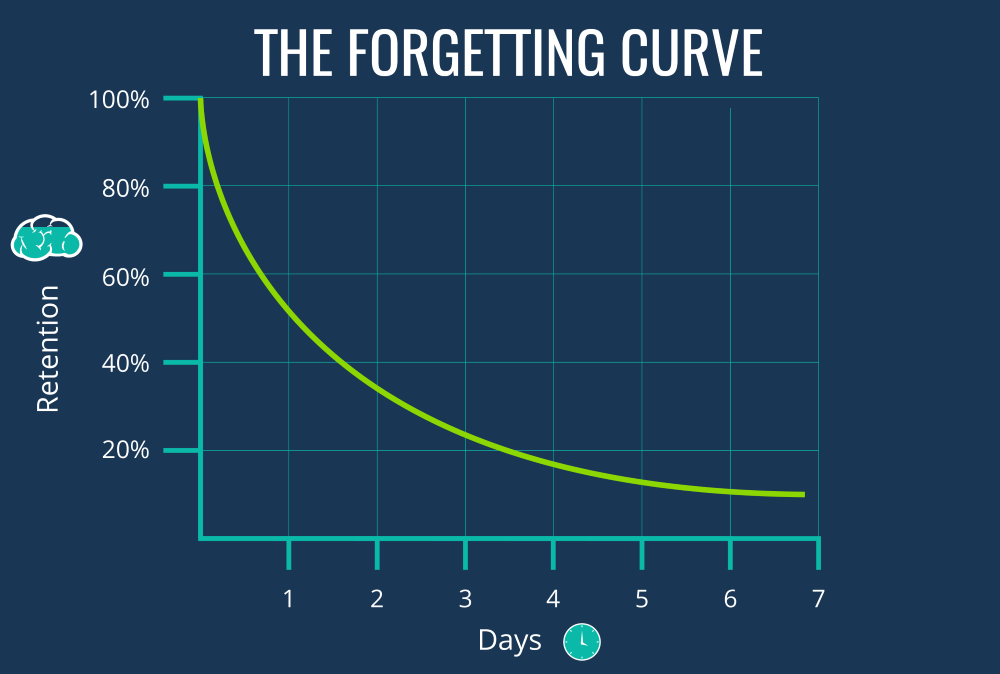
\includegraphics[width=13cm]{images/the-forgetting-curve.png}
\caption{Đường cong quên lãng.}
\label{fig_forgetting_curve}
\end{figure}
Quy luật tự nhiên này chỉ ra rằng nếu không có sự can thiệp kịp thời, phần lớn kiến thức sẽ biến mất chỉ sau một thời gian ngắn. Để đối phó với hiện tượng quên lãng, kỹ thuật lặp lại có khoảng cách (Spaced Repetition - SRS) đã ra đời như một giải pháp dựa trên bằng chứng khoa học \cite{Cepeda2008}. Thay vì nhồi nhét thông tin trong một thời gian ngắn, SRS tập trung vào việc dàn trải các phiên ôn tập theo thời gian. Nguyên lý then chốt của kỹ thuật này là thực hiện truy hồi thông tin ngay tại thời điểm trí nhớ bắt đầu suy giảm. Mỗi lần truy hồi thành công tại "điểm nút" này không chỉ khôi phục trí nhớ mà còn làm chậm đáng kể tốc độ quên lãng sau đó, giúp củng cố thông tin từ trí nhớ ngắn hạn sang trí nhớ dài hạn một cách bền vững \cite{Karpicke2008}.

Hiệu quả của mô hình SRS trong hệ thống này được hiện thực hóa thông qua thuật toán SM-2 (SuperMemo-2). Đây là một mô hình toán học cho phép cá nhân hóa hoàn toàn lộ trình học tập dựa trên khả năng phản hồi của từng cá nhân. Khác với các cơ chế nhắc nhở cố định, SM-2 vận hành dựa trên sự biến thiên của chỉ số độ dễ (Easiness Factor - EF) — đại lượng đại diện cho độ phức tạp của một từ vựng đối với một người học cụ thể. Thông qua điểm số chất lượng phản hồi ($q$) từ 0 đến 5, hệ thống sẽ liên tục điều chỉnh $EF$ theo công thức:

$$EF' = EF + (0.1 - (5 - q) \times (0.08 + (5 - q) \times 0.02))$$

Dựa trên chỉ số này, khoảng cách giữa các lần ôn tập ($I$) sẽ được mở rộng dần theo cấp số nhân. Trong đó, lần ôn tập thứ nhất ($I_1$) thường là sau 1 ngày, lần thứ hai ($I_2$) là 6 ngày, và từ lần thứ $n$ trở đi, khoảng cách được tính theo công thức $I_n = I_{n-1} \times EF$. Một đặc điểm quan trọng của thuật toán là việc duy trì ngưỡng $EF \ge 1.3$ — giá trị này không bao giờ được phép rơi dưới mức này, ngay cả khi người học trả lời sai nhiều lần. Ràng buộc này đảm bảo rằng ngay cả những từ vựng khó nhất vẫn được ôn tập với tần suất hợp lý, tránh việc khoảng cách ôn tập bị nén quá mức — điều dễ dẫn đến cảm giác nhàm chán và ảnh hưởng tiêu cực đến động lực học tập dài hạn.

Sự linh hoạt của SM-2 nằm ở cơ chế "thử thách vừa đủ": nếu người học trả lời sai ($q < 3$), thuật toán sẽ lập tức thiết lập lại chu kỳ về 0, buộc từ vựng đó phải xuất hiện thường xuyên hơn để củng cố lại dấu vết trí nhớ. Ngược lại, những từ vựng dễ sẽ được đẩy xa hơn trong lịch trình, giúp tối ưu hóa thời gian và công sức. Sự kết hợp giữa quy luật tâm lý học của Ebbinghaus và tính chính xác của thuật toán SM-2 tạo nên một động lực học tập dựa trên sự tiến bộ thực tế, đặt nền móng cho việc xây dựng thói quen ghi nhớ bền vững trong hệ thống.


\section{Lý thuyết Gamification và Cơ chế Thúc đẩy Động lực}

Mặc dù các giải pháp kỹ thuật như SM-2 đã tối ưu hóa được lộ trình ghi nhớ, thách thức lớn nhất vẫn nằm ở việc duy trì sự kiên trì của người học trước những rào cản về mặt tâm lý. Để giải quyết vấn đề này, Gamification được tích hợp nhằm bổ sung cơ chế trò chơi vào quy trình học tập để duy trì sự tham gia của người dùng \cite{Deterding2011}. Bằng cách lồng ghép các yếu tố đặc trưng của trò chơi, hệ thống hỗ trợ quá trình nội tâm hóa động lực học tập theo phổ của SDT \cite{Hamari2014}. Nhằm hạn chế các tác động tiêu cực của áp lực thành tích, hệ thống vận dụng khung lý thuyết Thuyết Tự Quyết (Self-Determination Theory - SDT) làm cơ sở thiết kế \cite{RyanDeci2017}.

Cốt lõi của SDT nhấn mạnh rằng động lực bền vững được hình thành khi các nhu cầu tâm lý cơ bản được đáp ứng. Trong đó, cảm giác về \textbf{Sự thành thạo (Competence)} được củng cố thông qua hệ thống phản hồi. Điểm tích lũy và hệ thống thăng cấp được thiết kế để phản ánh tiến trình phát triển năng lực, giúp người học nhận diện sự tiến bộ và duy trì động lực.

Tính \textbf{Tự quyết (Autonomy)} trong hệ thống được thể hiện qua quyền tự do xây dựng kho học liệu. Thay vì tuân theo một khuôn mẫu cố định, người dùng được chủ động biên soạn kho từ vựng cá nhân và lựa chọn thú ảo \cite{WerbachHunter2012}. Sự tự chủ này giúp người học chủ động hơn trong việc xây dựng lộ trình học tập theo nhu cầu cá nhân. Đồng thời, nhu cầu về \textbf{Sự kết nối (Relatedness)} được đáp ứng qua môi trường tương tác cộng đồng. Các bảng xếp hạng không chỉ khích lệ cạnh tranh mà còn tạo ra môi trường tương tác xã hội, qua đó đáp ứng nhu cầu gắn kết theo SDT.

Đặc điểm thiết kế trọng tâm của Gamification trong hệ thống là cơ chế thú ảo: khác với mô hình đặt streak (chuỗi ngày học liên tục) làm cơ chế gắn kết chủ đạo --- nơi một ngày bỏ học là thất bại hoàn toàn --- hệ thống xác định sự tăng trưởng của thú ảo là trục động lực trung tâm. Streak vẫn được ghi nhận như một chỉ số bổ sung về tính kỷ luật, nhưng điểm khác biệt then chốt là XP tích lũy cho thú ảo không bao giờ mất đi dù người học gián đoạn --- sự tiến hóa diễn ra theo quy luật tích lũy thuần túy, không có hình phạt hồi quy. Việc chuyển hóa nỗ lực học tập thành sự phát triển của thú ảo giúp giảm bớt áp lực tâm lý, thúc đẩy sự gắn kết với quá trình học tập. Cần lưu ý rằng, theo phổ liên tục của SDT \cite{RyanDeci2017}, phần thưởng ngẫu nhiên (cơ chế xác suất bắt thú) thuộc nhóm điều tiết ngoại tại, trong khi sự tiến hóa theo XP tích lũy --- gắn trực tiếp với nỗ lực học thuật --- hướng tới nhóm điều tiết đã được nội tâm hóa, tức người học tự nhận thấy giá trị của hoạt động. Sự kết hợp giữa hai mức độ điều tiết này nhằm hỗ trợ quá trình chuyển hóa từ động lực bên ngoài sang động lực bên trong theo phổ SDT.

\section{Vai trò của sự đối kháng và cạnh tranh}

Trong cấu trúc của hệ thống, chế độ chiến đấu (Battle Mode) không đơn thuần được thiết kế như một tính năng giải trí bề nổi, mà là ứng dụng có chủ đích của các nguyên lý khoa học giáo dục nhằm hỗ trợ quá trình tiếp thu ngôn ngữ.

Luận điểm đầu tiên nằm ở việc vận dụng Thuyết Xung đột Nhận thức (Cognitive Conflict Theory) \cite{Limon2001} kết hợp với khái niệm "Khó khăn thử thách có chủ đích" (Desirable Difficulties) \cite{Bjork2011}. Trong các trận đấu PvP/PvE, người học phải đồng thời xử lý kiến thức từ vựng và ra quyết định chiến thuật — chẳng hạn lựa chọn hệ thú theo nguyên tắc khắc chế (Lửa khắc Cỏ, Cỏ khắc Nước, Nước khắc Lửa) — trong khoảng thời gian hạn chế. Áp lực kép này buộc não bộ phải truy hồi từ vựng có chủ đích dưới điều kiện cạnh tranh, hiện thực hóa đúng bản chất của thực hành truy hồi chủ động. Nghiên cứu của Karpicke và Roediger \cite{Karpicke2008} chỉ ra rằng việc truy xuất thông tin dưới áp lực thời gian mang lại hiệu quả ghi nhớ dài hạn vượt trội so với học tập thụ động, kết quả được Carpenter \cite{Carpenter2012} xác nhận thêm trong bối cảnh học ngôn ngữ.


Bên cạnh đó, hệ thống tận dụng Thuyết Gắn kết Xã hội (Social Interdependence Theory) \cite{Johnson2009} để chuyển hóa các tương tác cạnh tranh thành động lực tự thân. Thông qua các bảng xếp hạng công khai và đấu trường trực tuyến, việc học không còn là một quá trình đơn độc mà gắn liền với vị thế xã hội trong một cộng đồng ảo. Theo SDT của Ryan và Deci \cite{RyanDeci2017}, sự cạnh tranh lành mạnh này thỏa mãn nhu cầu về năng lực (competence) và sự gắn kết (relatedness), từ đó thúc đẩy người học duy trì kỷ luật học tập một cách tự nguyện và bền bỉ hơn. Các nghiên cứu thực nghiệm của Hamari et al. \cite{Hamari2014} cũng chỉ ra rằng các yếu tố trò chơi hóa (gamification) có tác động tích cực đến thái độ và hành vi của người dùng khi được thiết kế đúng cách \cite{Deterding2011}.

Cuối cùng, sự đối kháng được tinh chỉnh để đưa người học vào Trạng thái Dòng chảy (Flow State) \cite{Csikszentmihalyi1990} thông qua hệ thống Gym Leader với độ khó tăng dần. Việc cân bằng giữa kỹ năng hiện tại của người học và thử thách của trò chơi là yếu tố then chốt để duy trì sự tập trung cực độ, tránh gây ra cảm giác nhàm chán hoặc lo âu quá mức \cite{WerbachHunter2012}. Cơ chế này biến việc truy hồi từ vựng thành yếu tố quyết định kết quả trận đấu, tạo động cơ ôn tập cụ thể. Cách tiếp cận này không chỉ nâng cao hiệu quả sư phạm mà còn hiện thực hóa mô hình học tập chủ động \cite{Prince2004}, giúp người học làm chủ kiến thức thông qua quá trình vận dụng trực tiếp vào các tình huống thực tế trong hệ thống \cite{Nation2001}.
\section{Các công trình và ứng dụng liên quan}

Việc ứng dụng các lý thuyết khoa học nhận thức như lặp lại ngắt quãng và thực hành truy hồi vào giáo dục ngôn ngữ đã được minh chứng qua sự thành công của nhiều nền tảng số. Tuy nhiên, qua quá trình khảo sát và phân tích các ứng dụng tiêu biểu, kết quả cho thấy vẫn tồn tại những rào cản nhất định trong việc cân bằng giữa hiệu quả học thuật và sự gắn kết cảm xúc bền vững.

Điển hình là trường hợp của \textbf{Duolingo}, nền tảng dẫn đầu về việc vận dụng các chỉ số định lượng như điểm kinh nghiệm (XP), bảng xếp hạng và chuỗi ngày học tập (streak) để duy trì thói quen người dùng. Mặc dù phương thức này tạo ra động lực tiếp cận ban đầu rất tốt, nhưng dưới góc độ tâm lý học hành vi, việc quá chú trọng vào các chỉ số ngoại tại dễ dẫn đến trạng thái áp lực tinh thần. Hệ quả là khi chuỗi ngày học tập bị đứt quãng, người học thường rơi vào trạng thái kiệt sức học tập và có xu hướng từ bỏ lộ trình thay vì tái kết nối \cite{DuolingoBlog2024}. Đây chính là \textbf{khoảng trống về tính bền vững của động lực}: hệ thống đang ưu tiên việc duy trì con số hơn là xây dựng một sợi dây liên kết nội tại giữa người học và tiến trình phát triển cá nhân.

Trong khi đó, \textbf{Quizlet} lại tiếp cận theo hướng đề cao quyền tự chủ, cho phép cá nhân hóa tối đa kho học liệu thông qua các bộ flashcard tự tạo \cite{QuizletLearn2024}. Tuy nhiên, điểm yếu cố hữu của mô hình này là sự vắng bóng của các cơ chế Gamification chuyên sâu, khiến nó dừng lại ở mức một công cụ hỗ trợ thuần túy. Sự thiếu hụt trong việc thỏa mãn đồng bộ ba nhu cầu cơ bản của thuyết Tự quyết (SDT) — bao gồm năng lực, tự chủ và sự gắn kết — dẫn đến việc người học cần một tinh thần tự giác cực cao để không bỏ dở giữa chừng.

Ở một thái cực khác, các công cụ như \textbf{Anki} và \textbf{Memrise} lại tập trung tối đa vào tính chính xác của thuật toán SRS để tối ưu hóa khả năng ghi nhớ dài hạn \cite{AnkiWeb2024, MemriseHelp2024}. Dù đạt hiệu quả cao về mặt kỹ thuật, nhóm ứng dụng này thường gặp rào cản lớn về trải nghiệm người dùng (UX) do giao diện khô khan và thiếu đi tính tương tác xã hội. Việc thiếu vắng yếu tố tự sự (narrative) và cơ chế phản hồi thiếu đa dạng khiến quy trình học tập trở nên đơn điệu, thiếu phản hồi tích cực.

Nhận diện khoảng trống nói trên, hệ thống được xây dựng nhằm tạo ra môi trường học tập nơi thuật toán SRS vận hành gắn liền với tiến trình phát triển của thú ảo, để mỗi từ vựng được ghi nhớ đóng góp trực tiếp vào sự phát triển đó.

Từ việc phân tích trên, có thể tổng kết \textbf{ba khoảng trống nghiên cứu (Research Gaps)} chính mà các hệ thống hiện tại chưa giải quyết triệt để:

\begin{itemize}
\item \textbf{Thiếu cơ chế gắn kết tích lũy bền vững:} Các hệ thống hiện có đặt streak (chuỗi ngày học liên tục) làm cơ chế gắn kết chủ đạo, khiến sự gián đoạn học tập --- điều không thể tránh trong thực tế --- trở thành tác nhân trực tiếp phá vỡ động lực. Khoảng trống này là cơ sở để thiết kế hệ thống với trục gắn kết dựa trên tích lũy XP không hồi quy (pet XP không bao giờ bị mất), kết hợp với hệ thống nhiệm vụ hàng ngày tạo các mốc ngắn hạn, thay vì phụ thuộc vào mô hình streak thuần túy.
\item \textbf{Sự mất cân bằng trong Gamification:} Phần lớn ứng dụng chỉ tập trung vào một vài yếu tố bề nổi (XP, Leaderboard, Streak) mà chưa triển khai hài hòa cả ba nhu cầu tâm lý cơ bản của Thuyết Tự Quyết (SDT): năng lực (competence), tự chủ (autonomy) và gắn kết (relatedness). Đặc biệt, tính tự chủ trong hầu hết các ứng dụng bị thu hẹp trong phạm vi lựa chọn nội dung, chứ chưa mở rộng sang quyền định hình hành trình học tập theo cách có ý nghĩa cá nhân.
\item \textbf{Sự thiếu hụt mô hình tích hợp SRS và Gamification:} Trong phạm vi các ứng dụng được khảo sát, chưa tìm thấy hệ thống nào tích hợp đồng thời: thuật toán SRS theo chuẩn SM-2, cơ chế Gamification gắn với thú ảo theo mô hình SDT, và tích lũy tiến trình không hồi quy. Nhận định này dựa trên phân tích tính năng công khai của các ứng dụng; so sánh có kiểm chứng là hướng nghiên cứu cần tiếp nối.
\end{itemize}

Đây chính là điểm cốt lõi mà hệ thống hướng tới: xây dựng cơ chế tích lũy có phản hồi trực quan, trong đó tiến trình học tập gắn liền trực tiếp với sự phát triển của thú ảo nhằm cụ thể hóa nhu cầu về năng lực (Competence) theo SDT.

\section{Hệ sinh thái công nghệ triển khai}

Để hiện thực hóa các mục tiêu về trải nghiệm tương tác tức thời và đảm bảo tính ổn định lâu dài cho hệ thống, việc lựa chọn nền tảng kỹ thuật được cân nhắc dựa trên sự giao thoa giữa hiệu năng vận hành và khả năng bảo trì mã nguồn. Cấu trúc công nghệ cốt lõi của dự án được định hình bởi bộ ba: ASP.NET Core điều phối logic tại tầng Backend, ReactJS (kết hợp cùng Vite và TypeScript) đảm nhiệm giao diện Frontend, và SQL Server chịu trách nhiệm quản trị dữ liệu quan hệ. Sự hội tụ của những công nghệ này cung cấp nền tảng kỹ thuật cho việc triển khai các tính năng đã đề ra và mở rộng trong các giai đoạn tiếp theo.

\subsection{Nền tảng Backend: ASP.NET Core}

Việc tin dùng ASP.NET Core làm "xương sống" cho tầng xử lý trung tâm xuất phát từ nhu cầu về một hệ thống có tính kỷ luật cao và hiệu suất thực thi mạnh mẽ. Cơ chế kiểm soát kiểu dữ liệu tĩnh của C\# giúp phát hiện sai sót tại giai đoạn biên dịch, hỗ trợ tái cấu trúc mã nguồn với độ an toàn cao hơn so với các ngôn ngữ kiểm soát kiểu động \cite{MicrosoftASPNETCore2024}. Đối với các tác vụ như tính toán lịch trình SRS và xử lý dữ liệu thời gian thực, framework vận hành hiệu quả nhờ mô hình bất đồng bộ tích hợp sẵn.

Các thành phần nội tại của framework được vận dụng cụ thể như sau. Cụ thể, máy chủ web Kestrel được triển khai để xử lý lưu lượng cao, hỗ trợ các kết nối WebSocket cần thiết cho việc cập nhật điểm số và kết quả quiz theo thời gian thực \cite{KestrelDocs2024}. Kiến trúc Middleware được thiết kế theo dạng chuỗi nối tiếp, giúp tách biệt các lớp bảo mật JWT và xử lý ngoại lệ tập trung \cite{MiddlewareDocs2024}. Thêm vào đó, việc áp dụng mẫu thiết kế Dependency Injection tích hợp sẵn đã giúp chuẩn hóa mô hình Controller–Service–Repository, không chỉ nâng cao tính độc lập của các module để phục vụ kiểm thử mà còn giảm bớt rủi ro khi thay đổi logic nghiệp vụ. Lập trình bất đồng bộ (Async/Await) và Entity Framework Core hỗ trợ quản trị tài nguyên máy chủ và điều chỉnh lược đồ dữ liệu qua migrations \cite{MicrosoftEFCore2024}.

\subsection{Lớp giao diện tương tác: ReactJS}

Trong vai trò là cầu nối trực tiếp với người dùng, ReactJS được lựa chọn nhờ khả năng xây dựng giao diện tương tác với tốc độ phản hồi cao. Do đặc thù của dự án yêu cầu sự đồng bộ liên tục giữa tiến độ học và trạng thái sinh trưởng của thú ảo, cơ chế Virtual DOM của ReactJS phù hợp để xử lý các cập nhật giao diện phức tạp với hiệu suất ổn định \cite{ReactDocs2024}. Triết lý thiết kế dựa trên thành phần (Component-based) cho phép phân rã giao diện thành những khối chức năng độc lập, giúp việc tái sử dụng mã nguồn trở nên dễ dàng và đảm bảo sự đồng nhất về mặt thẩm mỹ cho toàn bộ ứng dụng UI trong dài hạn.

Khả năng duy trì sự ổn định cho các màn hình có mật độ tương tác dày đặc được đảm bảo bởi thuật toán Reconciliation, giúp tiết giảm tối đa các thao tác can thiệp trực tiếp vào DOM thực \cite{ReactVirtualDOM2024}. Việc quản lý trạng thái và các tác vụ ngoại vi (side-effects) được thực hiện một cách tường minh thông qua React Hooks, kết hợp cùng TypeScript để tạo ra một "màng lọc" lỗi kiểu dữ liệu ngay từ đầu. Để bứt phá về tốc độ phát triển, dự án tích hợp Vite như một công cụ đóng gói thế hệ mới, mang lại trải nghiệm lập trình mượt mà với tính năng thay đổi nóng (HMR) tức thì \cite{ViteDocs2024}. Tailwind CSS theo hướng utility-first được áp dụng để xây dựng giao diện đồng nhất và tương thích đa kích thước màn hình.

\subsection{Quản trị dữ liệu: SQL Server}

SQL Server được chọn nhờ sự tương thích tốt trong hệ sinh thái .NET và hỗ trợ tiêu chuẩn ACID đảm bảo tính nhất quán dữ liệu \cite{SQLServerDocs2024}. Trong bối cảnh giáo dục, tính toàn vẹn của dữ liệu lịch sử học tập là yêu cầu quan trọng; SQL Server đáp ứng yêu cầu này cùng các công cụ giám sát tích hợp. Sự kết hợp giữa các kỹ thuật tối ưu truy vấn hiện đại như Columnstore Index và khả năng vận hành linh hoạt trên môi trường đám mây giúp hệ thống đạt được sự cân bằng giữa tốc độ truy xuất và khả năng mở rộng quy mô.

\subsection{Các dịch vụ tích hợp đám mây}

Bên cạnh bộ ba nền tảng cốt lõi, hệ thống tích hợp một lớp dịch vụ đám mây chuyên biệt nhằm tự động hóa các tác vụ đòi hỏi năng lực xử lý vượt ra ngoài khả năng của một ứng dụng đơn lẻ.

\textbf{Google Gemini API} được tích hợp để sinh tự động các thuộc tính ngôn ngữ học của từ vựng, bao gồm phiên âm IPA, nghĩa tiếng Việt, câu ví dụ ngữ cảnh, từ loại và cấp độ CEFR tương ứng. Việc khai thác mô hình ngôn ngữ lớn (LLM) cho phép hệ thống cung cấp dữ liệu chất lượng cao mà không yêu cầu biên soạn thủ công, đồng thời cho phép mở rộng kho từ vựng mà không cần biên soạn thủ công.

\textbf{Azure AI Speech Services} cung cấp công nghệ tổng hợp giọng nói (Text-to-Speech) với giọng đọc chuẩn \texttt{en-US-AndrewNeural}, xuất tệp MP3 và lưu trữ trên Azure Blob Storage. Cơ sở hạ tầng CDN tích hợp của Azure đảm bảo tệp âm thanh được phân phối tới người dùng với độ trễ thấp, phục vụ trực tiếp cho loại câu hỏi nghe hiểu (Listening) trong các phiên học.

\textbf{Redis} đóng vai trò là lớp bộ nhớ đệm phân tán (Distributed Cache) thông qua giao diện \texttt{IDistributedCache} của ASP.NET Core. Kết quả sinh metadata từ Gemini API được lưu vào bộ nhớ đệm với thời gian tồn tại 7 ngày, giúp loại bỏ các lần gọi API trùng lặp và giảm đáng kể chi phí vận hành. Hệ thống được thiết kế theo nguyên tắc xuống cấp nhẹ nhàng (graceful degradation): khi Redis không khả dụng, luồng xử lý tiếp tục bình thường thông qua API trực tiếp mà không gây gián đoạn dịch vụ.

\subsection{Phân tích tổng hợp}

Kết hợp giữa ASP.NET Core, ReactJS và SQL Server tạo thành một khung kỹ thuật ổn định cho việc triển khai các tính năng đã đặt ra. Trong khi tầng Backend xử lý các nghiệp vụ logic và dữ liệu tập trung, tầng Frontend ưu tiên tính đáp ứng trong trải nghiệm người dùng \cite{TechEmpower2024}.




\chapter{Hệ thống hỗ trợ học từ vựng tiếng Anh kết hợp Gamification}
\label{Chapter3}

Nội dung trọng tâm của Chương 3 tập trung vào công tác phân tích kỹ thuật và hoạch định cấu trúc cho hệ thống. Dựa trên các cơ sở khoa học về nhận thức cùng lý thuyết trò chơi hóa đã được thiết lập tại Chương~\ref{Chapter2}, chương này sẽ cụ thể hóa các giải pháp thông qua việc xác định hệ thống yêu cầu nghiệp vụ và các tiêu chuẩn vận hành kỹ thuật. Từ đó, các mô hình kiến trúc, quy trình xử lý dữ liệu và cấu trúc lưu trữ sẽ được xây dựng một cách chi tiết và logic.

Giai đoạn phân tích đóng vai trò là nhịp cầu kết nối, giúp chuyển đổi các khái niệm học thuật như lặp lại ngắt quãng hay thực hành truy hồi thành các module chức năng có tính khả thi cao về mặt triển khai. Trên nền tảng đó, phần thiết kế sẽ khái quát hóa kiến trúc tổng thể, minh họa qua hệ thống sơ đồ UML và cấu trúc cơ sở dữ liệu quan hệ. Toàn bộ các nội dung này tạo thành một khung tham chiếu kỹ thuật chặt chẽ, định hướng trực tiếp cho quá trình xây dựng và hoàn thiện sản phẩm ở các giai đoạn tiếp theo.

\section{Phân tích yêu cầu}

Công tác phân tích yêu cầu đóng vai trò then chốt trong việc chuyển hóa các mục tiêu lý thuyết thành những đặc tính kỹ thuật cụ thể cho hệ thống. Qua quá trình khảo sát thực tiễn và nghiên cứu mô hình, các yêu cầu của hệ thống được phân định rõ rệt nhằm đảm bảo khả năng vận hành toàn diện.

\subsection{Yêu cầu chức năng}

Đối với người học, chức năng cốt lõi tập trung vào việc cá nhân hóa kho học liệu và tham gia chia sẻ cộng đồng. Quá trình học tập được hiện thực hóa thông qua các phiên học đa dạng, tích hợp cùng lịch nhắc tự động dựa trên thuật toán SRS nhằm tối ưu hóa ghi nhớ dài hạn \cite{Cepeda2008}. Các cơ chế trò chơi hóa như tích lũy điểm thưởng và nâng cấp thú ảo được lồng ghép để duy trì động lực nội tại theo thuyết SDT \cite{RyanDeci2017}.

Đối với quản trị viên, hệ thống trang bị công cụ giám sát người dùng và điều phối quyền truy cập. Nhiệm vụ trọng tâm bao gồm quản lý kho từ vựng chuẩn và tinh chỉnh thông số Gamification để tối ưu hóa trải nghiệm \cite{Deterding2011}. Phân hệ báo cáo cung cấp dữ liệu thống kê chuyên sâu, hỗ trợ đánh giá hiệu quả học tập và cải tiến vận hành kịp thời.

\subsection{Yêu cầu phi chức năng}

Về phương diện hiệu năng, hệ thống xác lập các tiêu chuẩn vận hành khắt khe nhằm đảm bảo sự mượt mà trong tương tác, với thời gian phản hồi mục tiêu duy trì ổn định dưới ngưỡng 3 giây cho mọi tác vụ truy vấn \cite{TechEmpower2024}. An ninh hệ thống được thiết lập làm trọng tâm phát triển thông qua việc áp dụng các cơ chế mã hóa mật khẩu hiện đại và thiết lập hàng rào bảo mật API dựa trên giao thức xác thực JSON Web Token (JWT), đảm bảo tính toàn vẹn và quyền riêng tư của dữ liệu người học \cite{MiddlewareDocs2024}. Cấu trúc hệ thống được quy hoạch theo mô hình module hóa, cho phép linh hoạt trong việc mở rộng quy mô tải trọng mà không làm gián đoạn dòng chảy dịch vụ \cite{MicrosoftASPNETCore2024}. Bên cạnh đó, tính khả dụng của nền tảng được tối ưu hóa thông qua thiết kế đáp ứng, đảm bảo sự đồng nhất về trải nghiệm thị giác trên cả môi trường máy tính và các thiết bị di động cầm tay \cite{ReactDocs2024}.

\section{Thiết kế hệ thống chi tiết}
\subsection{Kiến trúc tổng thể}

Kiến trúc của hệ thống được phát triển dựa trên sự kế thừa và tối ưu hóa mô hình ba lớp – một chuẩn mực trong việc xây dựng các ứng dụng Client-Server đòi hỏi tính tin cậy và khả năng xử lý tải trọng lớn \cite{MicrosoftASPNETCore2024}. Sự phân định rạch ròi giữa các tầng Giao diện (Presentation), tầng Xử lý nghiệp vụ (Application) và tầng Dữ liệu (Data) không chỉ tạo ra sự độc lập về mặt thực thi công nghệ mà còn gia tăng hiệu quả bảo trì, cho phép phân tách trách nhiệm trong chu kỳ phát triển phần mềm.

Lớp Giao diện (Frontend) được định hình trên nền tảng ReactJS cùng sự hỗ trợ từ hệ sinh thái công cụ tân tiến bao gồm Vite, TypeScript và TailwindCSS, hướng tới mục tiêu kiến tạo một môi trường học tập có độ phản hồi cao \cite{ReactDocs2024, ViteDocs2024}. Việc triển khai kiến trúc dựa trên thành phần (Component-based) của ReactJS giúp module hóa các đơn vị giao diện, cho phép tái sử dụng mã nguồn và giảm thiểu đáng kể độ phức tạp trong quản trị cấu trúc UI \cite{ReactVirtualDOM2024}. Tính chặt chẽ của TypeScript kết hợp cùng tốc độ biên dịch từ Vite giúp củng cố độ ổn định và gia tăng hiệu suất lập trình \cite{TypeScriptDocs2024}. Trong dòng vận hành, Frontend đóng vai trò là thực thể tương tác trực tiếp, giao tiếp với Backend qua hệ thống RESTful API để thực thi các nghiệp vụ lõi: từ việc truy xuất học liệu đến điều phối các phiên quiz đa tương tác, đồng thời trực quan hóa các biến động về tiến trình và trạng thái thú ảo theo thời gian thực nhằm duy trì động lực nội tại cho người dùng \cite{Hamari2014}.

Tại trung tâm điều phối của hệ thống, lớp Xử lý nghiệp vụ (Backend) được thực thi qua ASP.NET Core Web API, đảm nhận trọng trách quản trị luồng dữ liệu và thực thi logic nghiệp vụ phức hợp \cite{MicrosoftASPNETCore2024}. Từ quản lý định danh người dùng đến các thuật toán tính toán điểm thưởng và logic tiến hóa thú ảo đều được đóng gói tập trung tại đây. Backend thể hiện tính linh hoạt thông qua cấu trúc Middleware Pipeline, cho phép tích hợp các quy trình kiểm soát xuyên suốt như xác thực JWT, logging hệ thống và xử lý ngoại lệ tập trung \cite{MiddlewareDocs2024}. Thêm vào đó, việc sử dụng Entity Framework Core theo phương thức Code-First giúp thiết lập sự đồng bộ nhịp nhàng giữa các mô hình đối tượng C\# và cấu trúc dữ liệu vật lý \cite{MicrosoftEFCore2024}. Với thiết kế RESTful chuẩn hóa, hệ thống đảm bảo khả năng cung ứng dữ liệu đa nền tảng với hiệu năng ấn tượng, đáp ứng kỳ vọng về trải nghiệm người dùng hiện đại \cite{TechEmpower2024}.

\newpage
Tầng Dữ liệu (Data Layer) ứng dụng hệ quản trị SQL Server để lưu trữ bền vững toàn bộ dữ liệu, đặc biệt là các bản ghi chi tiết về lịch sử học tập phục vụ cho thuật toán lặp lại ngắt quãng \cite{SQLServerDocs2024, MemriseHelp2024}. Lược đồ dữ liệu được quy hoạch theo cấu trúc quan hệ chặt chẽ cùng các ràng buộc toàn vẹn để loại bỏ các rủi ro về sai lệch logic. Nhằm sẵn sàng cho các tác vụ báo cáo và phân tích sâu, các thực thể dữ liệu được chuẩn hóa tối ưu, hỗ trợ khả năng truy vấn hiệu quả ngay cả khi quy mô người dùng mở rộng. Toàn bộ kiến trúc này phối hợp qua giao thức an toàn HTTP/HTTPS, tạo nên một hệ thống vừa vững chắc về kỹ thuật, vừa linh hoạt trong môi trường triển khai thực tế.

\subsubsection{Kiến trúc Frontend module hóa — Component-Based Architecture}

Kiến trúc Frontend của hệ thống được tổ chức theo triết lý đóng gói và tái sử dụng, hướng tới sự bền vững trong việc mở rộng tính năng. Cấu trúc mã nguồn được phân rã thành các lớp chức năng dựa trên nguyên lý kiến trúc sạch (Clean Architecture). Tại tầng thành phần (Components), các đơn vị giao diện cơ bản được thiết kế độc lập hoàn toàn với logic nghiệp vụ, đảm bảo khả năng tích hợp linh hoạt. Đối với các module chức năng (Features/Pages), hệ thống tổ chức theo từng phân hệ riêng biệt như: quản lý học tập, hệ thống thú ảo hay hồ sơ năng lực. Mỗi module này là một đơn vị tự bao đóng, tích hợp các trang chính, thành phần đặc thù và các Custom Hooks để quản trị trạng thái nội bộ \cite{ReactDocs2024}.

Giao thức giao tiếp với lớp Server được tập trung hóa tại tầng dịch vụ (Services/Hooks), nơi các Axios client được cấu hình theo từng nhóm API tương ứng. Đặc biệt, hệ thống tích hợp SignalR tại tầng này để duy trì các kênh truyền tải dữ liệu thời gian thực cho chế độ chiến đấu PvP. Việc quản lý trạng thái toàn cục (State Management) được thực thi qua Redux, đảm bảo tính nhất quán cho các thông tin quan trọng như quyền truy cập hay tiến độ học thuật. Cuối cùng, lớp hỗ trợ (Utilities/Types) xác lập hệ thống kiểu dữ liệu nghiêm ngặt qua TypeScript, đảm bảo tính an toàn kiểu cho các thuật toán phức tạp như SM-2 ngay tại phía Client \cite{TypeScriptDocs2024}. Cách tiếp cận này không chỉ hỗ trợ tốt cho việc kiểm thử tự động với Jest mà còn đảm bảo hệ thống luôn trong trạng thái minh bạch, dễ dàng bảo trì và cập nhật.

\subsubsection{Kiến trúc Backend chi tiết — Clean Architecture \& Design Patterns}

Backend của hệ thống được hiện thực hóa dựa trên kiến trúc Onion (Clean Architecture), một tư duy thiết kế tiên tiến tập trung vào việc tách biệt hoàn toàn logic nghiệp vụ khỏi các phụ thuộc về framework hay hạ tầng kỹ thuật. Toàn bộ mã nguồn được tổ chức thành bốn lớp đồng tâm với nguyên tắc phụ thuộc hướng tâm, đảm bảo tính bền vững trước những thay đổi công nghệ.

\begin{figure}[H]
\centering
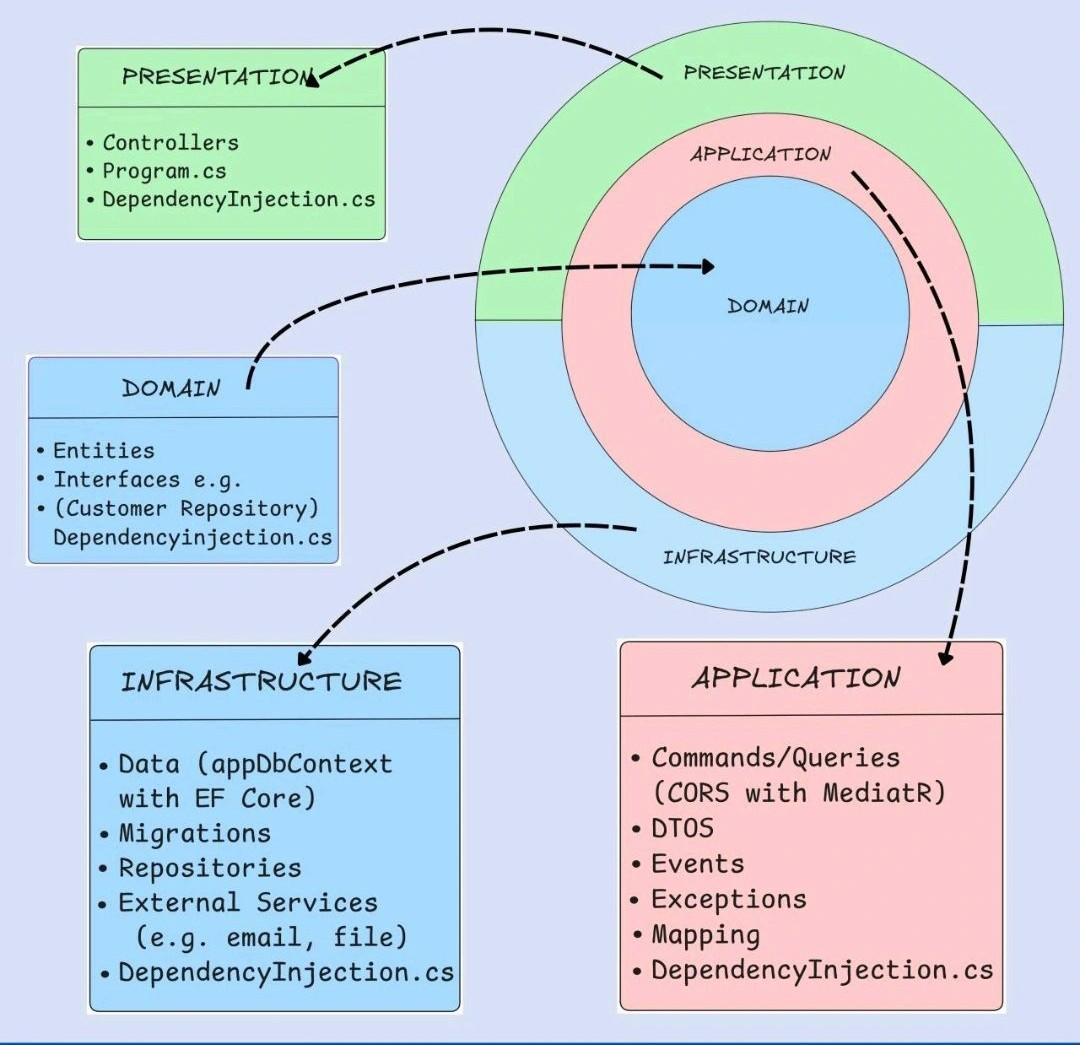
\includegraphics[width=15cm]{images/clean-architecture.jpg}
\caption{Kiến trúc Clean (Onion Architecture) triển khai trong hệ thống.}
\label{fig_clean_architecture}
\end{figure}

\newpage
Lớp nhân (Domain Layer) đóng vai trò là "trái tim" của hệ thống, chứa đựng các thực thể (Entities) và quy tắc nghiệp vụ cốt lõi mà không phụ thuộc vào bất kỳ thư viện bên thứ ba nào. Tại đây, hơn 25 thực thể chính đại diện cho các khái niệm như người dùng, từ vựng và tiến trình học tập được định nghĩa, kết hợp cùng các Domain Services để xử lý các thuật toán phức tạp như lịch trình ôn tập SM-2. Bao quanh lớp nhân là lớp ứng dụng (Application Layer), đóng vai trò điều phối luồng dữ liệu giữa Domain và các thành phần ngoại vi. Lớp này chứa các dịch vụ ứng dụng để chiết xuất logic nghiệp vụ, sử dụng các đối tượng chuyển đổi dữ liệu (DTOs) để bảo vệ cấu trúc nội bộ và định nghĩa các Interfaces làm hợp đồng cho các lớp bên ngoài thực thi.

Lớp hạ tầng (Infrastructure Layer) chịu trách nhiệm hiện thực hóa các Interfaces từ lớp ứng dụng, quản lý việc tương tác với cơ sở dữ liệu SQL Server thông qua Entity Framework Core và các dịch vụ ngoại vi như Cloudinary hay hệ thống gửi thông báo \cite{MicrosoftEFCore2024}. Tại lớp này, mẫu thiết kế Repository và Unit of Work được áp dụng một cách chiến lược. Với 23 Repositories riêng biệt được quản lý tập trung qua Unit of Work, hệ thống đảm bảo tính nguyên tử (Atomicity) của các giao dịch dữ liệu và tối ưu hóa việc quản lý bộ nhớ thông qua cơ chế tải trễ (lazy-loading). Cuối cùng, lớp trình diễn (Presentation Layer) đóng vai trò là điểm tiếp nhận yêu cầu duy nhất, nơi các Controllers tiếp nhận HTTP requests, xử lý xác thực JWT qua Middleware và điều phối công việc tới các dịch vụ ứng dụng tương ứng \cite{MiddlewareDocs2024}. Việc áp dụng cơ chế Dependency Injection xuyên suốt tất cả các lớp đã tạo ra một hệ thống lỏng lẻo (loose coupling), cho phép giả lập dữ liệu (mocking) dễ dàng để đạt được tỉ lệ bao phủ Unit Test cao, đồng thời sẵn sàng cho việc thay đổi công nghệ lưu trữ mà không gây ảnh hưởng đến logic nghiệp vụ hiện hữu.

Tóm lại, sự phối hợp giữa cấu trúc Frontend dựa trên thành phần và Backend theo kiến trúc Onion đã tạo nên một đơn vị phần mềm vững chắc. Sự kết hợp này không chỉ đáp ứng trọn vẹn các yêu cầu chức năng về học tập và Gamification mà còn thiết lập một nền tảng kỹ thuật chuẩn mực, đảm bảo khả năng vận hành ổn định và sẵn sàng cho các giai đoạn phát triển mở rộng trong thực tế.

\subsection{Mô hình hóa chức năng qua sơ đồ Use Case}

Kiến trúc chức năng của hệ thống được trực quan hóa thông qua sơ đồ Use Case tại Hình~\ref{fig_uc}. Đây là tài liệu kỹ thuật quan trọng nhằm xác lập ranh giới vận hành và các luồng tương tác giữa các chủ thể tham gia vào hệ thống. Việc xây dựng mô hình này không chỉ giúp định hình phạm vi nghiệp vụ mà còn đảm bảo sự giao thoa hài hòa giữa các nguyên lý giáo dục hiện đại và cơ chế trò chơi hóa, tạo tiền đề vững chắc cho công tác thiết kế cấu trúc dữ liệu ở các giai đoạn tiếp theo.

\begin{figure}[H]
\centering
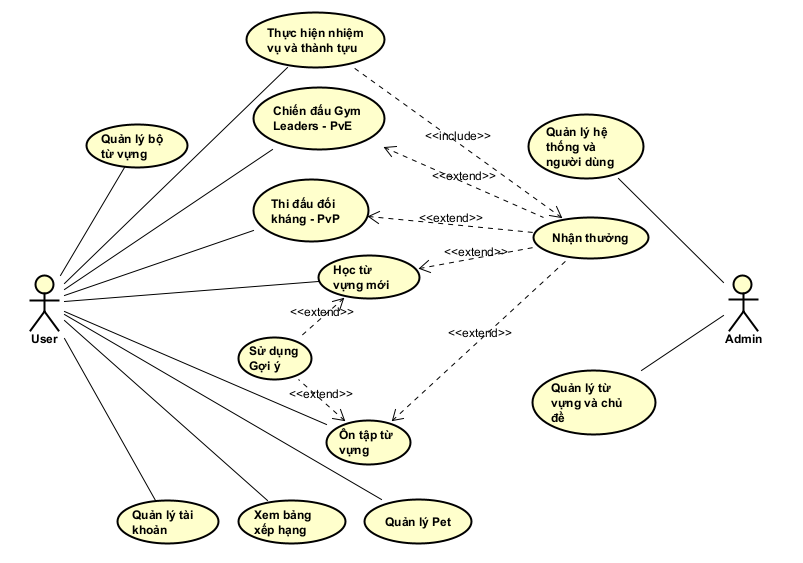
\includegraphics[width=15cm]{images/FinalUseCase.png}
\caption{Sơ đồ Use Case tổng thể của hệ thống.}
\label{fig_uc}
\end{figure}

\textbf{Hệ thống các tác nhân (Actors)}

Hệ thống phân định rõ hai nhóm chủ thể tương tác với những phạm vi quyền hạn và trách nhiệm chuyên biệt:
\begin{itemize}
    \item \textbf{Người dùng (User):} Là hạt nhân trung tâm của ứng dụng. Tác nhân này trực tiếp tham gia vào lộ trình học thuật và trải nghiệm các phân hệ giải trí. Quyền hạn của người dùng được giới hạn trong phạm vi quản lý dữ liệu cá nhân, bao gồm tiến trình ghi nhớ từ vựng, quản lý thú ảo (Pet) và các chỉ số tích lũy cá nhân.
    \item \textbf{Quản trị viên (Admin):} Đảm nhận vai trò điều hành và duy trì tính toàn vẹn của nền tảng. Admin chịu trách nhiệm kiểm soát chất lượng kho học liệu, phê duyệt chủ đề, giám sát hoạt động hệ thống và tinh chỉnh các tham số vận hành nhằm đảm bảo môi trường học tập luôn ổn định và an toàn.
\end{itemize}

\newpage
\textbf{Cấu trúc các phân hệ chức năng}

Nhằm tối ưu hóa trải nghiệm người dùng và đảm bảo hiệu quả trong công tác quản trị, các chức năng của hệ thống được cấu trúc chặt chẽ thành ba phân hệ logic. Trung tâm của hệ thống là phân hệ Quản lý và Học tập, đóng vai trò thực thi các phương pháp sư phạm cốt lõi thông qua việc cung cấp học liệu theo chủ đề. Tại đây, thuật toán lặp lại ngắt quãng được áp dụng để cá nhân hóa lộ trình, giúp tối ưu hóa khả năng ghi nhớ dài hạn dựa trên các nguyên lý khoa học nhận thức. Song song đó, phân hệ này còn đảm nhận vai trò quản trị tài khoản, cho phép người dùng đăng ký, đăng nhập và tự quản lý hồ sơ năng lực cá nhân một cách an toàn.

Để duy trì sự gắn kết, Hệ sinh thái Gamification và Tương tác được thiết lập như một lớp động lực thúc đẩy hành vi học tập tự thân. Người dùng chuyển hóa thành quả tri thức thành các nguồn tài nguyên để phát triển thú ảo, tạo ra sợi dây liên kết cảm xúc giữa nỗ lực học thuật và sự tăng trưởng của các thực thể số. Các chế độ thi đấu PvE và PvP không chỉ đơn thuần là tính năng giải trí mà còn đóng vai trò là các bài kiểm tra năng lực thời gian thực, buộc người học phải vận dụng kiến thức dưới áp lực cạnh tranh.

Cuối cùng, Module Điều hành hệ thống cung cấp bộ công cụ toàn diện cho tác nhân quản trị. Phân hệ này cho phép quản lý linh hoạt kho dữ liệu từ vựng và thiết lập các thuộc tính chiến đấu cho hệ thống thú ảo. Quản trị viên cũng có khả năng can thiệp vào các thông số cân bằng trò chơi như phần thưởng hoặc sự kiện để duy trì tính hấp dẫn và ổn định cho cộng đồng người dùng.

\textbf{Các mối quan hệ và ràng buộc nghiệp vụ}

Sơ đồ Use Case vận dụng các quan hệ \textbf{include} và \textbf{extend} để làm rõ các điều kiện logic và sự phụ thuộc giữa các chức năng. Quan hệ \textbf{include} (Bao hàm) được áp dụng cho các tiến trình mang tính bắt buộc: ví dụ, cơ chế nhận thưởng luôn gắn liền với việc hoàn tất một nhiệm vụ cụ thể. Điều này đảm bảo tính chặt chẽ trong việc ghi nhận thành tích người dùng.

Ngược lại, quan hệ \textbf{extend} (Mở rộng) mô tả các hành vi có tính điều kiện hoặc không bắt buộc. Điển hình là chức năng "Sử dụng trợ giúp" (Hint) chỉ phát sinh khi người học gặp khó khăn trong phiên ôn tập. Tương tự, hành động "Nhận thưởng" được thiết kế như một phần mở rộng từ các kết quả thành công trong học tập hoặc thi đấu, giúp hệ thống duy trì tính linh hoạt. Việc phân định rõ rệt các mối quan hệ này giúp kiến trúc phần mềm đạt được sự minh bạch và dễ dàng bảo trì trong tương lai.

\subsection{Thiết kế phân quyền theo vai trò}

Việc bảo vệ các tài nguyên nhạy cảm của hệ thống được giải quyết thông qua mô hình phân quyền dựa trên vai trò. Thay vì kiểm tra quyền tại từng phương thức riêng lẻ, ASP.NET Core cho phép khai báo chính sách bảo mật tập trung ngay tại cấp độ lớp bằng thuộc tính [Authorize(Roles = "...")], sau đó Middleware Pipeline xác thực JWT tự động thực thi chính sách này trước khi bất kỳ luồng nghiệp vụ nào được khởi chạy \cite{MiddlewareDocs2024}.

Hệ thống phân định ba cấp độ vai trò với phạm vi quyền tăng dần. Vai trò \textbf{User} là mức mặc định dành cho người học, giới hạn trong phạm vi các endpoint học tập, đối kháng và quản lý tài sản cá nhân. Vai trò \textbf{Admin} mở rộng quyền ra các tác vụ quản trị nội dung — quản lý từ vựng, nhiệm vụ hàng ngày, thành tích và cấu hình Gym Leader. Vai trò \textbf{SuperAdmin} ở cấp cao nhất, kế thừa toàn bộ quyền của Admin đồng thời có quyền độc quyền truy cập vào các endpoint vận hành hạ tầng: cấu hình hệ thống, kiểm tra sức khỏe (Health Check) và bảo trì tự động (xả Redis cache, dọn dẹp cơ sở dữ liệu cũ).

Thông tin vai trò được ASP.NET Core Identity ghi vào JWT dưới dạng claim chuẩn tại thời điểm đăng nhập. Phía ứng dụng quản trị, thông tin này được đọc trực tiếp từ token bằng thư viện jwtDecode nhằm điều chỉnh động giao diện điều hướng — tài khoản \textbf{Admin} thấy các nhóm mục User Management và Content, trong khi \textbf{SuperAdmin} thấy thêm hai nhóm chỉ dành riêng: System (Thông báo, Bảng xếp hạng PvP, Xem lại trận đấu, Phân tích phiên học) và Settings (System Health, System Config, Logs, Generals). Mọi yêu cầu vào hệ thống đều phải thông qua lớp kiểm tra claim này; bất kỳ token nào không thuộc hai vai trò trên sẽ bị từ chối ngay tại bước khởi tạo phiên.

\subsection{Sơ đồ tuần tự}

Sơ đồ tuần tự đóng vai trò quan trọng trong việc mô hình hóa các tương tác động giữa các đối tượng trong hệ thống theo trình tự thời gian, qua đó làm rõ luồng xử lý của các nghiệp vụ phức tạp từ phía giao diện đến tầng lưu trữ dữ liệu.


\subsubsection{Quy trình tạo bộ từ vựng}

\begin{figure}[H]
\centering
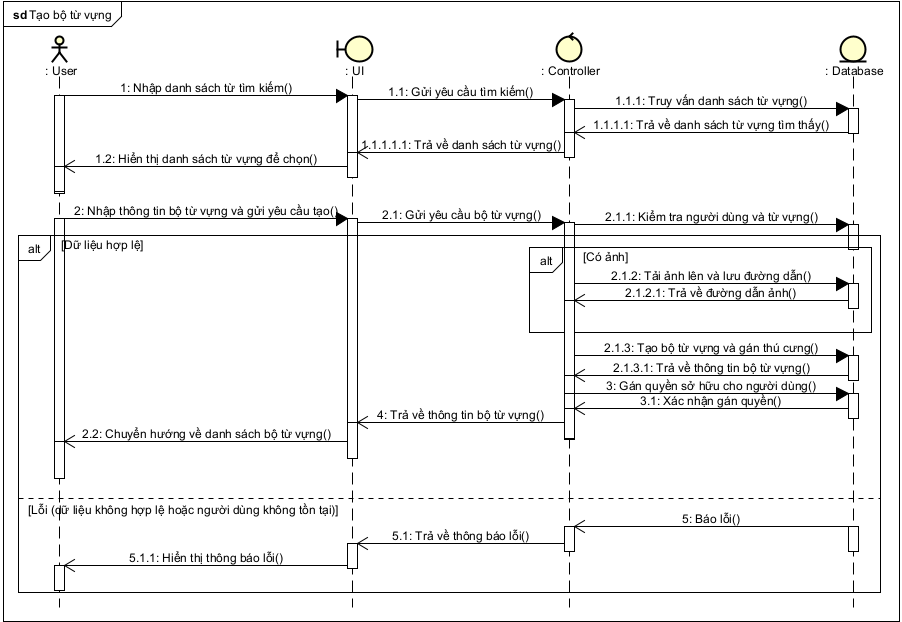
\includegraphics[width=15cm]{images/Final_Sq_Set.png}
\caption{Sơ đồ tuần tự quy trình tạo bộ từ vựng.}
\label{fig_seq2}
\end{figure}

Tiến trình khởi tạo bộ từ vựng bắt đầu từ giao diện bốn bước: người dùng lần lượt xác lập metadata (tiêu đề, chủ đề, độ khó, chế độ công khai), nhập danh sách từ vựng thô qua bàn phím hoặc tệp .csv/.txt, xem xét và chỉnh sửa bản dự thảo AI, rồi xác nhận tạo. Sau khi UI gửi yêu cầu tới AiPreviewVocabularySetAsync, Controller kiểm tra cache Redis — nếu kết quả AI cho từ đó đã tồn tại (thời gian lưu: 7 ngày), phản hồi được trả lại ngay lập tức mà không cần gọi Gemini. Mỗi phần tử trong danh sách dự thảo mang cờ isExisting để phân biệt từ đã có trong hệ thống, hoặc isAiGenerated cho từ mới vừa được AI sinh metadata.

Sau khi người dùng hoàn chỉnh bản dự thảo, yêu cầu tạo (AiCreateVocabularySetAsync) được gửi lên Backend xử lý. Controller kiểm tra tính toàn vẹn dữ liệu, đồng thời điều phối dịch vụ Cloudinary để lưu trữ ảnh đại diện và AzureSpeechService để tổng hợp âm thanh cho từng từ mới. Các từ có isExisting = true được liên kết trực tiếp vào bộ từ mà không tạo bản ghi trùng lặp; các chỉnh sửa của người dùng trên những từ này được lưu vào bảng \textbf{SetVocabulary} thay vì bảng \textbf{Vocabularies} gốc. Khi dữ liệu được xác nhận hợp lệ, một bản ghi bộ từ mới được tạo lập trong cơ sở dữ liệu, đồng thời hệ thống dựa vào ThemeToPetTypesMap để tự động gán các \textbf{SetRewardPet} phù hợp với chủ đề, kích hoạt cơ chế Gamification ngay từ giai đoạn khởi đầu. Quy trình này đảm bảo tính nhất quán của dữ liệu hệ thống và thúc đẩy quyền tự chủ (Autonomy) của người học trong việc xây dựng lộ trình kiến thức cá nhân \cite{RyanDeci2017}.


\subsubsection{Quy trình thực hiện trận đấu}

\begin{figure}[H]
\centering
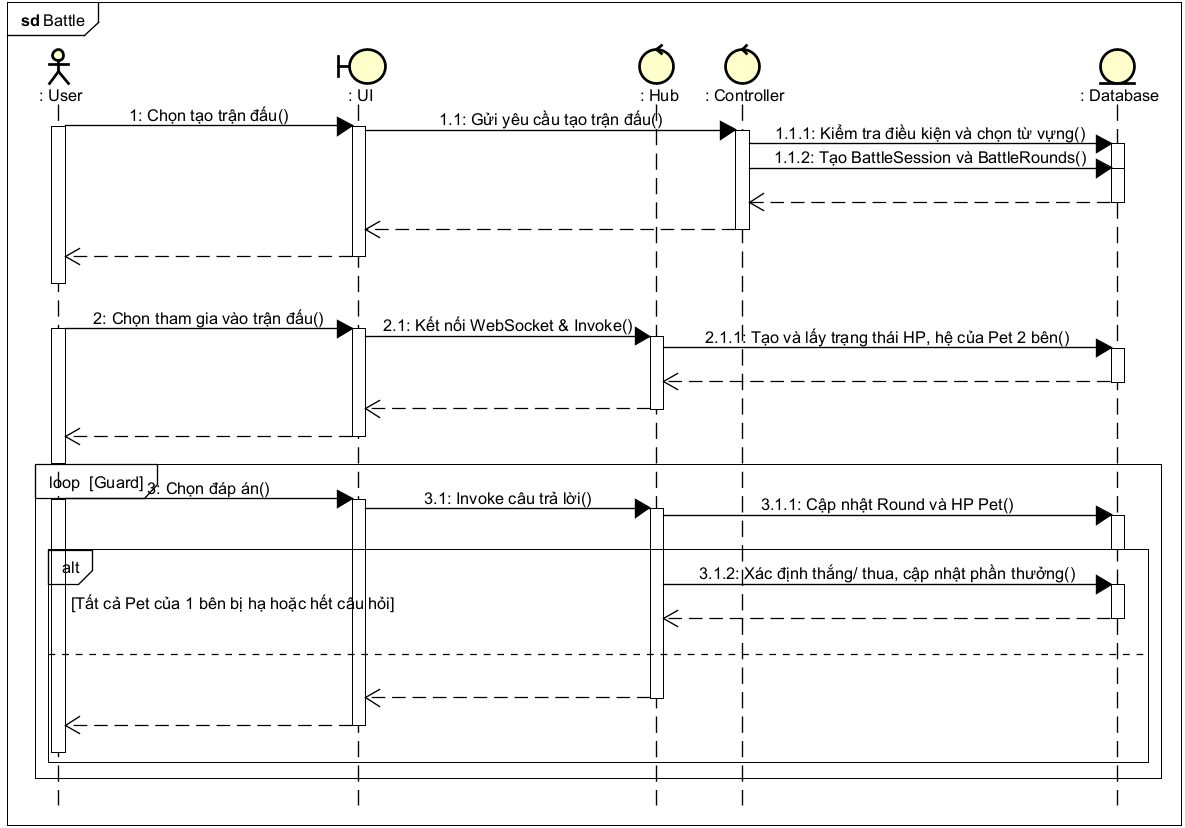
\includegraphics[width=15cm]{images/Final_Sq_Battle.png}
\caption{Sơ đồ tuần tự quy trình thực hiện trận đấu.}
\label{fig_seq3}
\end{figure}

Quy trình chiến đấu thời gian thực thể hiện sự phối hợp phức tạp giữa các giao thức truyền tải dữ liệu khác nhau. Khởi đầu trận đấu, người chơi lựa chọn đội hình thú cưng, sau đó Controller thông qua Service sẽ khởi tạo một phiên đấu và các vòng đấu tương ứng trong Database. Mã định danh phiên đấu sau đó được sử dụng để thiết lập kết nối WebSocket thông qua SignalR Hub, cho phép duy trì luồng dữ liệu song công với độ trễ thấp.

Trong suốt vòng lặp thi đấu, các chỉ số về HP, thuộc tính hệ và câu hỏi tương tác được đồng bộ liên tục giữa Server và Client. Logic chấm điểm được thực hiện tập trung tại Server dựa trên tính chính xác và tốc độ phản hồi của người chơi, giúp đảm bảo tính công bằng và ngăn chặn các hành vi gian lận phía Client. Khi trận đấu kết thúc do một bên bị hạ gục hoặc hết câu hỏi, hệ thống sẽ thực hiện tính toán các phần thưởng nâng cao như điểm ELO (đối với PvP) hoặc huy hiệu thành tựu (đối với PvE). Sự kết hợp giữa kiến trúc RESTful cho các tác vụ khởi tạo và WebSockets cho các tương tác thời gian thực mang lại một trải nghiệm giải trí học thuật liền mạch và lôi cuốn \cite{WerbachHunter2012, Deterding2011}.


\subsubsection{Quy trình học, ôn từ vựng và nhận thưởng}

\begin{figure}[H]
\centering
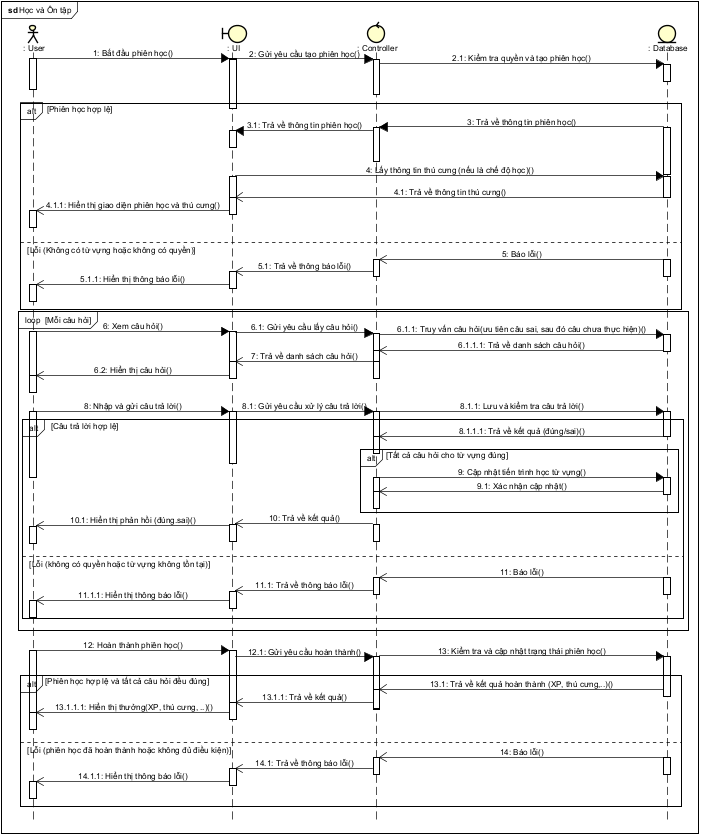
\includegraphics[width=13cm]{images/Final_Sq_HocvaOntap.png}
\caption{Sơ đồ tuần tự quy trình học, ôn tập từ vựng và nhận thưởng.}
\label{fig_seq1}
\end{figure}
Tiến trình vận hành của một phiên tương tác kiến thức được khởi tạo khi người dùng lựa chọn bộ học liệu mục tiêu. Tại tầng Backend, Controller kiểm tra sự tồn tại của session chưa hoàn thành — nếu có, trả về session cũ cùng tiến trình đã lưu; nếu chưa, hệ thống tạo session mới. Trong phiên học mới (Learning), 5 từ chưa tiếp cận được chọn và một thú ảo phần thưởng được xác định theo mốc tích lũy; đồng thời buff của thú ảo đang kích hoạt được đọc một lần và ghi vào session record — bao gồm cả việc tính CatchRate += PetCatchBonus ngay tại thời điểm này.

Trong giai đoạn tương tác lõi, mỗi từ vựng phải vượt qua bốn cấp độ câu hỏi tăng dần. Mỗi phản hồi được lưu ngay vào \textbf{AnswerRecord} kèm thời gian phản hồi và số gợi ý đã dùng. Khi từ vựng hoàn thành cả bốn cấp trong phiên ôn tập (Review), hệ thống tính grade SM-2 dựa trên số lần sai, thời gian trung bình và số gợi ý, sau đó gọi ISRSService.UpdateAfterReviewAsync để điều chỉnh EaseFactor và lịch ôn tập tiếp theo, toàn bộ được lưu vào \textbf{VocabularyReviewHistory}.

Giai đoạn kết thúc phiên học thực thi chuỗi nghiệp vụ Gamification theo thứ tự: cộng XP đã nhân buff vào tài khoản, kiểm tra và cấp thú ảo phần thưởng (chỉ phiên Learning), cộng 100 XP thú ảo đang kích hoạt có thể dẫn tới tiến hóa, cập nhật tiến trình nhiệm vụ hàng ngày và kiểm tra điều kiện mở khóa Gym Leader mới dưới dạng tác vụ bất đồng bộ không chờ kết quả. Cách thiết kế này đã hiện thực hóa thành công cơ chế truy hồi chủ động (Active Recall) \cite{Karpicke2008}, đồng thời vận dụng vòng lặp phản hồi tích cực để duy trì động lực nội tại \cite{Hamari2014}.


\subsection{Sơ đồ hoạt động}
Sơ đồ hoạt động (Activity Diagram) đóng vai trò là công cụ mô hình hóa trực quan, cung cấp một cái nhìn toàn diện và chi tiết về luồng điều khiển cũng như trình tự vận hành các quy trình nghiệp vụ bên trong hệ thống. Trong khi sơ đồ tuần tự (Sequence Diagram) tập trung khai thác các khía cạnh tương tác và trao đổi thông điệp giữa các thực thể theo trục thời gian, sơ đồ hoạt động lại ưu tiên mô tả logic thực thi từ góc độ quy trình (Workflow).

Cụ thể, các sơ đồ được trình bày dưới đây nhấn mạnh vào cấu trúc tuần tự của các thao tác kỹ thuật, các điểm phân nhánh điều kiện và các chu trình lặp lại của những tiến trình xử lý cốt lõi. Cách tiếp cận này giúp làm rõ cách thức hệ thống điều phối dữ liệu, xử lý các tình huống ngoại lệ và chuyển đổi trạng thái nghiệp vụ, từ đó đảm bảo tính nhất quán và chặt chẽ trong việc hiện thực hóa các chức năng phức tạp của phần mềm.
\subsubsection{Cơ chế thiết lập kho học liệu cá nhân}

\begin{figure}[H]
\centering
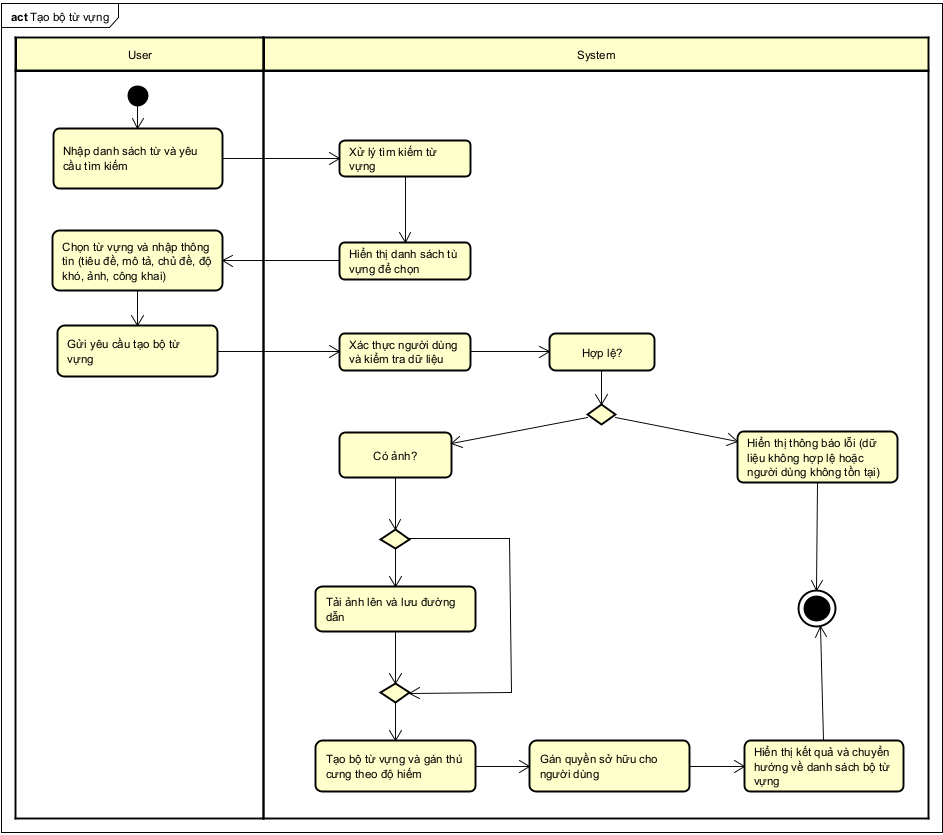
\includegraphics[width=15cm]{images/Final_AT_Set.png}
\caption{Sơ đồ luồng nghiệp vụ khởi tạo bộ từ vựng.}
\label{fig_act2}
\end{figure}

Sự hình thành của một bộ học liệu mới trong hệ thống là kết quả của quá trình cộng tác giữa các thao tác chủ động từ người dùng và các thủ tục kiểm soát chặt chẽ tại tầng Backend. Luồng nghiệp vụ được kích hoạt khi người dùng tiến hành tổng hợp các đơn vị từ vựng mục tiêu, đồng thời xác lập các thuộc tính định danh như tên gọi, phân loại chủ đề và ngưỡng độ khó mong muốn. Tại đây, hệ thống vận hành như một màng lọc để thẩm định tính toàn vẹn của dữ liệu đầu vào, đồng thời điều phối việc xử lý và lưu trữ các tài nguyên đa phương tiện đi kèm nhằm tối ưu hóa khả năng hiển thị.

Ngay sau khi các tiêu chuẩn xác thực được thỏa mãn, một thực thể dữ liệu mới sẽ được khởi tạo kèm theo cơ chế định danh quyền truy cập nghiêm ngặt. Một mắt xích quan trọng trong giai đoạn này là sự can thiệp của thuật toán gamification: hệ thống sẽ tự động thực hiện phép thử xác suất để liên kết bộ từ vựng với các sinh vật ảo dựa trên hệ số hiếm \cite{RyanDeci2017}. Việc lồng ghép yếu tố bất ngờ này ngay tại bước chuẩn bị không chỉ nâng cao giá trị sưu tầm mà còn tạo động lực tâm lý tích cực để người học bắt đầu lộ trình chinh phục kiến thức. Quy trình được khép lại bằng các tác vụ đồng bộ hóa cơ sở dữ liệu, đảm bảo rằng kho tri thức cá nhân luôn sẵn sàng cho các hoạt động học tập và chia sẻ cộng đồng về sau.

\subsubsection{Cơ chế điều phối và xử lý logic đối kháng}

\begin{figure}[H]
\centering
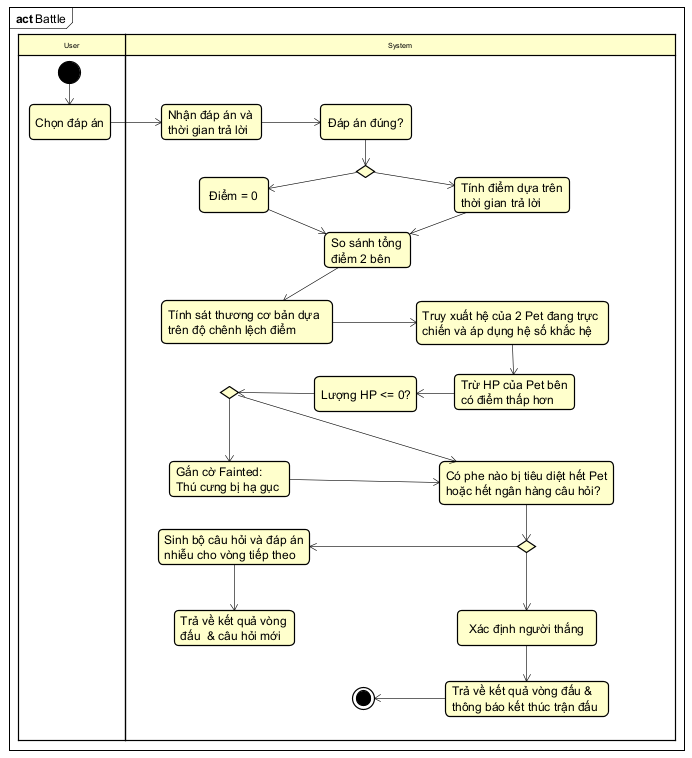
\includegraphics[width=12cm]{images/Final_AT_Battle.png}
\caption{Sơ đồ luồng nghiệp vụ xử lý trận đấu thời gian thực.}
\label{fig_act3}
\end{figure}

Trọng tâm vận hành của tính năng đối kháng được cụ thể hóa qua hàm xử lý SubmitAnswerAsync, nơi các tham số kỹ thuật được chuyển hóa thành tương tác trong trò chơi. Luồng xử lý được kích hoạt ngay khi hệ thống tiếp nhận phản hồi từ người dùng cùng dữ liệu về thời gian thực thi (ElapsedMs). Tại tầng xử lý trung tâm, một thuật toán phức hợp sẽ tính toán sát thương dựa trên sự giao thoa giữa độ chính xác và tốc độ phản xạ. Điểm nhấn tạo nên chiều sâu chiến thuật chính là việc áp dụng \textbf{Ma trận khắc chế thuộc tính}, cho phép các đặc tính nguyên tố của thú ảo trực tiếp tác động và nhân dồn chỉ số sát thương cuối cùng lên đối thủ \cite{Deterding2011}.

Sau khi cập nhật chỉ số sinh tồn (HP) của đối phương, hệ thống sẽ thực hiện các bước kiểm tra logic để xác định trạng thái tiếp theo của cuộc đấu. Trong trường hợp trận đấu vẫn tiếp diễn, một chu kỳ câu hỏi mới sẽ được khởi tạo với các phương án nhiễu (distractors) được sinh ngẫu nhiên nhằm duy trì tính thử thách. Khi các điều kiện kết thúc được thỏa mãn, Backend sẽ đảm nhiệm các nghiệp vụ hậu kỳ quan trọng như điều chỉnh chỉ số xếp hạng ELO hoặc ghi nhận các danh hiệu (Badge) cho người học. Mô hình tính toán tập trung tại Server này không chỉ bảo vệ tính toàn vẹn của kết quả mà còn nâng tầm hoạt động kiểm tra từ vựng thành một trải nghiệm thể thao điện tử đầy kịch tính \cite{Hamari2014, Bjork2011}.

\subsubsection{Hệ thống hóa quy trình tích lũy tri thức và quản lý phần thưởng}

\begin{figure}[H]
\centering
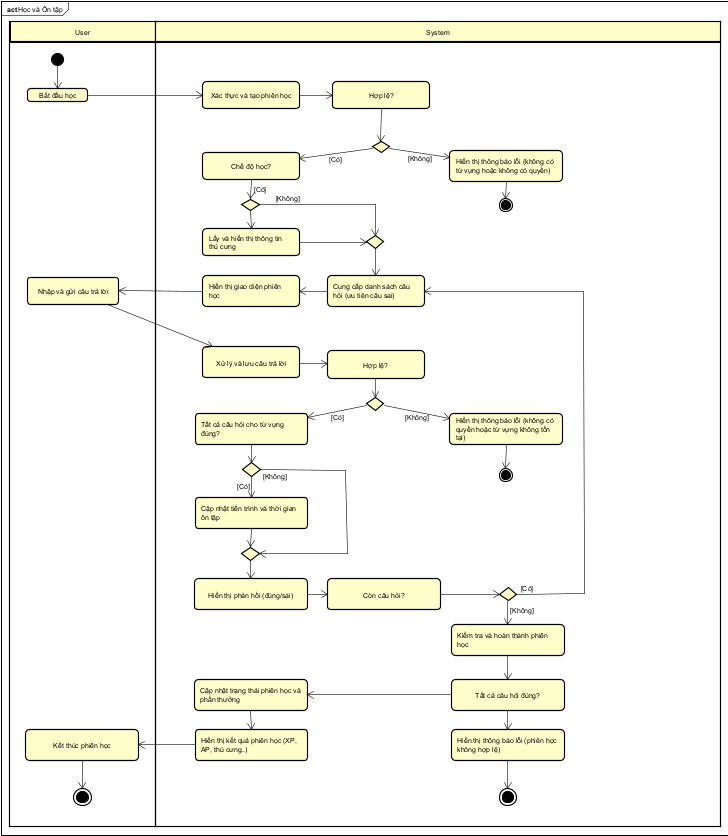
\includegraphics[width=13cm]{images/Final_AT_HocvaOntap.png}
\caption{Sơ đồ hoạt động quy trình học tập và cơ chế thúc đẩy hành vi.}
\label{fig_act1}
\end{figure}

Tiến trình củng cố kiến thức được thiết kế như một vòng lặp kín, bắt đầu từ việc thẩm định quyền truy cập và tính hợp lệ của phiên học mà người dùng yêu cầu. Hệ thống sẽ thực hiện phản hồi thông báo lỗi nếu các điều kiện tiền đề không được đáp ứng; ngược lại, một môi trường học tập cá nhân hóa sẽ được thiết lập, tích hợp sẵn các chỉ số trạng thái của thú ảo đồng hành.

Chiến lược phân phối nội dung được điều phối dựa trên cơ chế ưu tiên các đơn vị kiến thức chưa đạt ngưỡng ghi nhớ. Tại đây, sự tương tác hai chiều được duy trì liên tục: phản hồi từ người học sẽ ngay lập tức được hệ thống phân tích và trả về kết quả định hướng. Mắt xích quan trọng nhất của quy trình chính là việc điều chỉnh chu kỳ ôn tập dựa trên các câu trả lời chính xác tuyệt đối, đảm bảo tuân thủ nguyên tắc thực hành truy hồi chủ động để tối ưu hóa khả năng ghi nhớ dài hạn \cite{Karpicke2008}. Khi tất cả các đơn vị kiến thức trong phiên được xử lý, quy trình sẽ chuyển sang giai đoạn tổng kết. Tại đây, các chỉ số kinh nghiệm (XP) và các phần thưởng vật phẩm ảo sẽ được tính toán dựa trên hiệu suất thực tế, tạo ra một cơ chế phản hồi tích cực giúp người dùng tìm thấy sự khích lệ tự thân trong suốt lộ trình học tập \cite{WerbachHunter2012}.

\subsection{Sơ đồ trạng thái}

Sơ đồ trạng thái đóng vai trò mô hình hóa vòng đời của một thực thể từ vựng trong hệ thống, từ giai đoạn tiếp cận ban đầu đến khi đạt mức độ thành thạo dài hạn. Quá trình này được chia thành hai cấp độ quản lý: trạng thái tương tác trong phiên học và trạng thái lưu trữ theo thuật toán Spaced Repetition.

\subsubsection{Trạng thái từ vựng trong phiên học}

\begin{figure}[H]
\centering
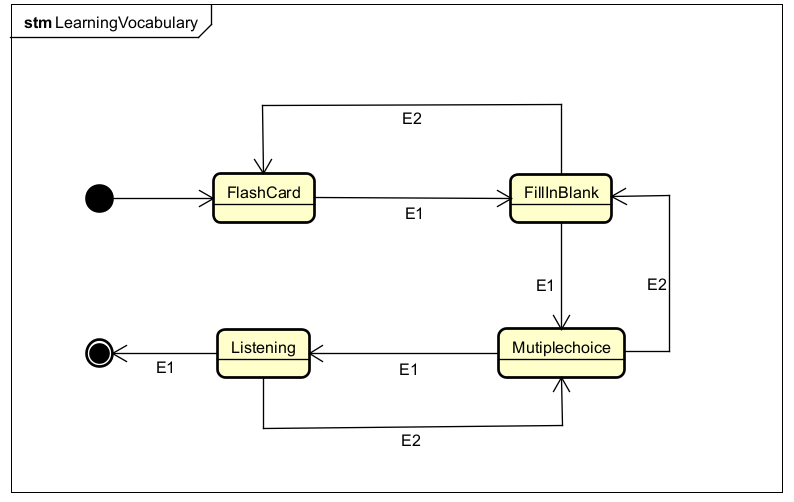
\includegraphics[width=14cm]{images/state.png}
\caption{Sơ đồ trạng thái từ vựng trong phiên học.}
\label{fig_session_state}
\end{figure}

Trong phạm vi một phiên học (Learning Session), mỗi từ vựng sẽ trải qua một chuỗi các trạng thái tương tác với độ khó tăng dần nhằm đảm bảo khả năng nhận diện và ghi nhớ toàn diện. Khởi đầu tại trạng thái Flashcard, người học thực hiện nhận diện mặt chữ và nghĩa của từ, sau đó tuần tự chuyển dịch qua các hình thức kiểm tra phức tạp hơn như điền từ vào chỗ trống (FillInBlank), lựa chọn đáp án đúng (MultipleChoice) và kỹ năng nghe hiểu (Listening).



Sự chuyển dịch giữa các trạng thái này được điều phối bởi hai sự kiện phản hồi chính: trả lời đúng (E1) và trả lời sai (E2). Khi sự kiện E1 xảy ra, hệ thống sẽ nâng bậc trạng thái, cho phép người học tiếp cận loại câu hỏi tiếp theo; ngược lại, sự kiện E2 sẽ kích hoạt cơ chế giảm trạng thái, buộc người học quay lại bước trước đó để củng cố kiến thức. Từ vựng chỉ được xác nhận là hoàn thành phiên học khi người học vượt qua tất cả các bậc thử thách một cách liên tục. Cơ chế này không chỉ cá nhân hóa lộ trình theo năng lực thực tế mà còn ngăn chặn triệt để tình trạng "học lướt", đảm bảo tính chắc chắn trong việc tiếp thu kiến thức mới \cite{Bjork2011}.

\subsubsection{Trạng thái từ vựng theo thuật toán SM-2}

\begin{figure}[H]
\centering
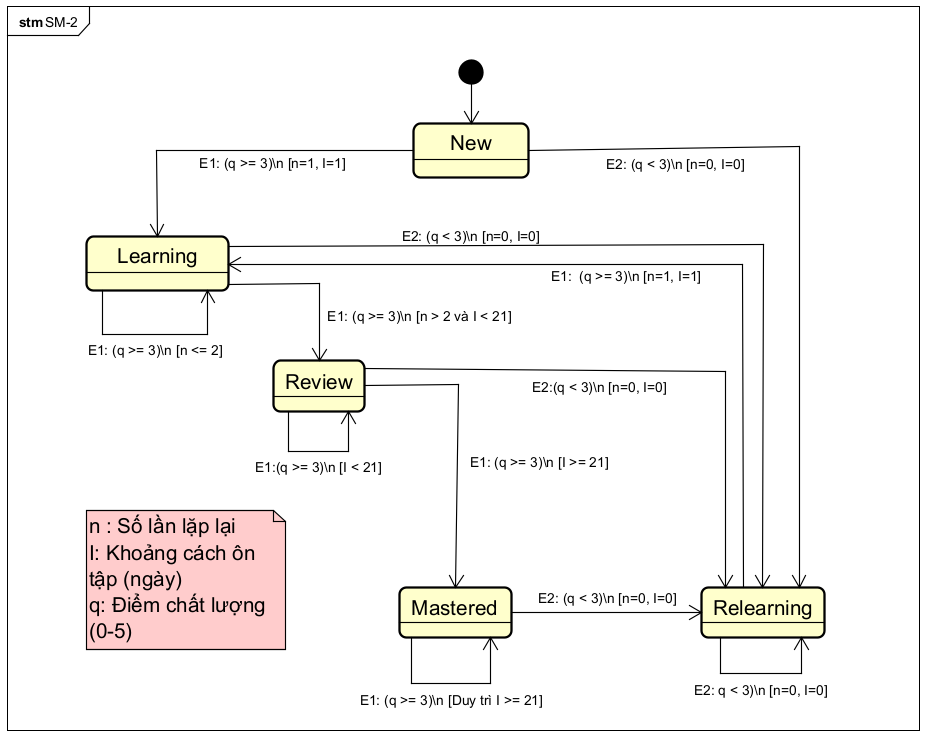
\includegraphics[width=14cm]{images/sm2state.png}
\caption{Sơ đồ trạng thái từ vựng theo thuật toán SM-2.}
\label{fig_sm2_state}
\end{figure}

\newpage
Ngoài các trạng thái tương tác tức thời, hệ thống còn quản lý sự chuyển dịch trạng thái của từ vựng trong trí nhớ dài hạn dựa trên thuật toán SM-2. Các trạng thái cốt lõi bao gồm: Mới (New), Đang học (Learning), Ôn tập (Review), Thành thạo (Mastered) và Học lại (Relearning). Mỗi phản hồi của người dùng không chỉ tác động đến phiên học hiện tại mà còn trực tiếp thay đổi các tham số toán học như số lần lặp lại ($n$), chỉ số độ dễ (EF) và khoảng cách ôn tập ($I$).

Điểm mấu chốt trong cơ chế chuyển dịch này nằm ở sự kiện trả lời sai (E2 - với điểm số $q < 3$). Khi đó, hệ thống thực hiện nghiệp vụ tái thiết lập (reset) số lần lặp lại và khoảng cách ôn tập về giá trị 0. Việc đưa khoảng cách về 0 đồng nghĩa với việc từ vựng sẽ được ưu tiên xuất hiện ngay trong phiên học kế tiếp để thực hiện quy trình chỉnh sửa lỗi sai (error correction) kịp thời. Ngược lại, khi người dùng trả lời đúng (E1), khoảng cách ôn tập sẽ được mở rộng theo cấp số nhân dựa trên chỉ số EF, dịch chuyển từ vựng dần sang trạng thái "Mastered" khi đạt ngưỡng $I \geq 21$ ngày. Quy trình này tuân thủ nghiêm ngặt nguyên lý học tập dựa trên sự khó khăn có chủ đích, giúp tối ưu hóa khả năng lưu trữ thông tin của não bộ và duy trì hiệu quả học tập bền vững \cite{Cepeda2008, Karpicke2008}.

\subsection{Phân tích cấu trúc thực thể và quan hệ logic}

Sơ đồ lớp (Class Diagram) được thiết lập như một bản thiết kế khung, phản ánh cấu trúc tĩnh và các mối liên kết nghiệp vụ giữa các thành phần trong hệ thống. Thông qua việc cụ thể hóa các khái niệm trừu tượng thành các thực thể lập trình tại tầng Domain, sơ đồ này đóng vai trò là kim chỉ nam cho quá trình triển khai mã nguồn và quản lý logic nghiệp vụ. Việc phân rã các lớp đối tượng theo từng phân hệ chức năng tuân thủ nguyên tắc phân tách trách nhiệm (Separation of Concerns), tạo điều kiện cho việc bảo trì và mở rộng hệ thống.

\subsubsection{Nhóm Quản lý người dùng và Xác thực}

\begin{figure}[H]
\centering
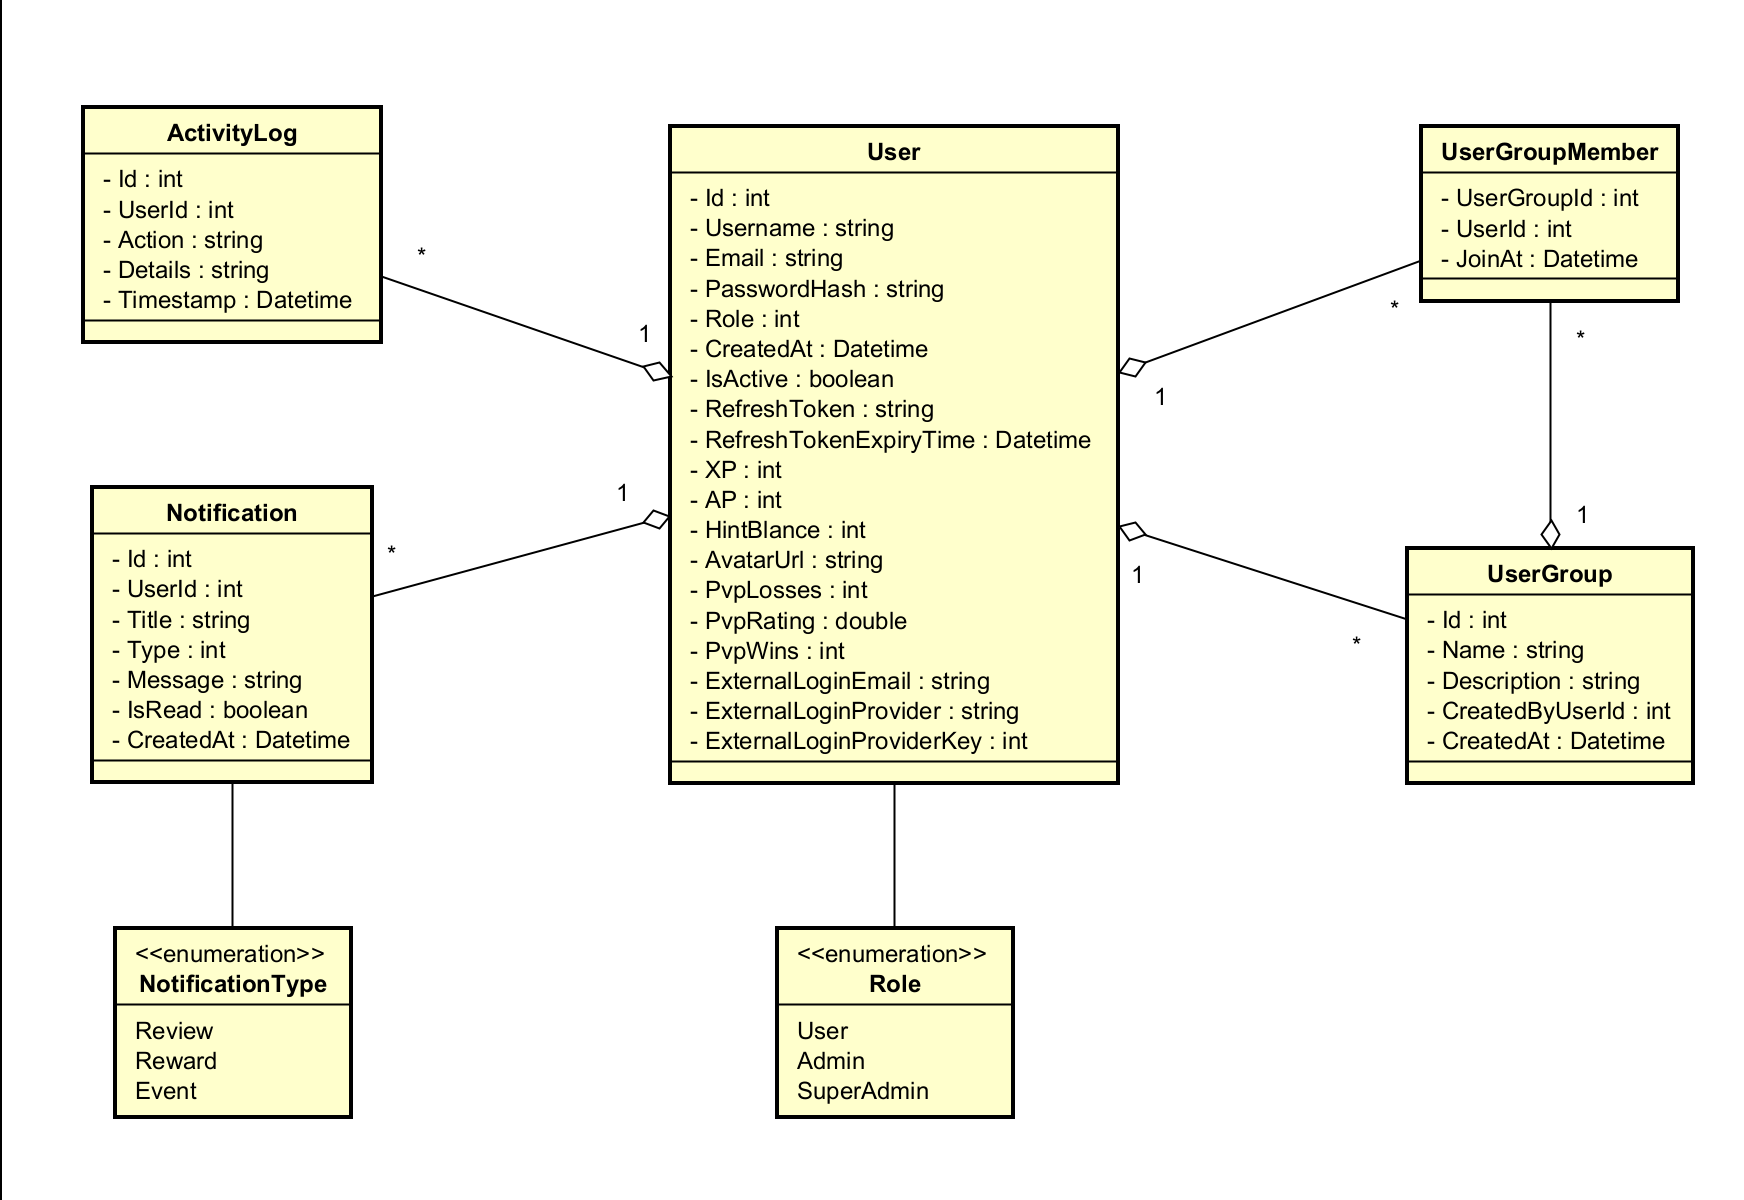
\includegraphics[width=15cm]{images/Class_User.png}
\caption{Sơ đồ lớp nhóm Quản lý người dùng và Xác thực.}
\label{fig_class_user}
\end{figure}

Thực thể \textbf{User} là trục trung tâm của toàn hệ thống, lưu trữ thông tin xác thực (Email, PasswordHash, RefreshToken), hồ sơ cá nhân (Username, AvatarUrl) và các chỉ số tiến triển (XP, AP, PvpRating, PvpWins, PvpLosses). \textbf{ActivityLog} ghi nhận nhật ký hoạt động với liên kết khóa ngoại tới User, phục vụ cho việc kiểm soát và phân tích hành vi người dùng. Hệ thống nhóm học tập được quản lý qua cặp thực thể \textbf{UserGroup} và \textbf{UserGroupMember}: UserGroup lưu tên, mô tả và người tạo nhóm (CreatedByUserId), còn UserGroupMember đóng vai trò bảng trung gian nhiều-nhiều giữa User và UserGroup, ghi nhận thời điểm tham gia (JoinedAt). Thực thể \textbf{Notification} phân loại các thông báo đẩy qua enum \textbf{NotificationType} (Review, Reward, Event). Phân quyền toàn hệ thống được điều phối bởi enum \textbf{UserRole} với ba cấp độ: User, Admin và SuperAdmin.

\subsubsection{Nhóm Từ vựng và Nội dung học liệu}

\begin{figure}[H]
\centering
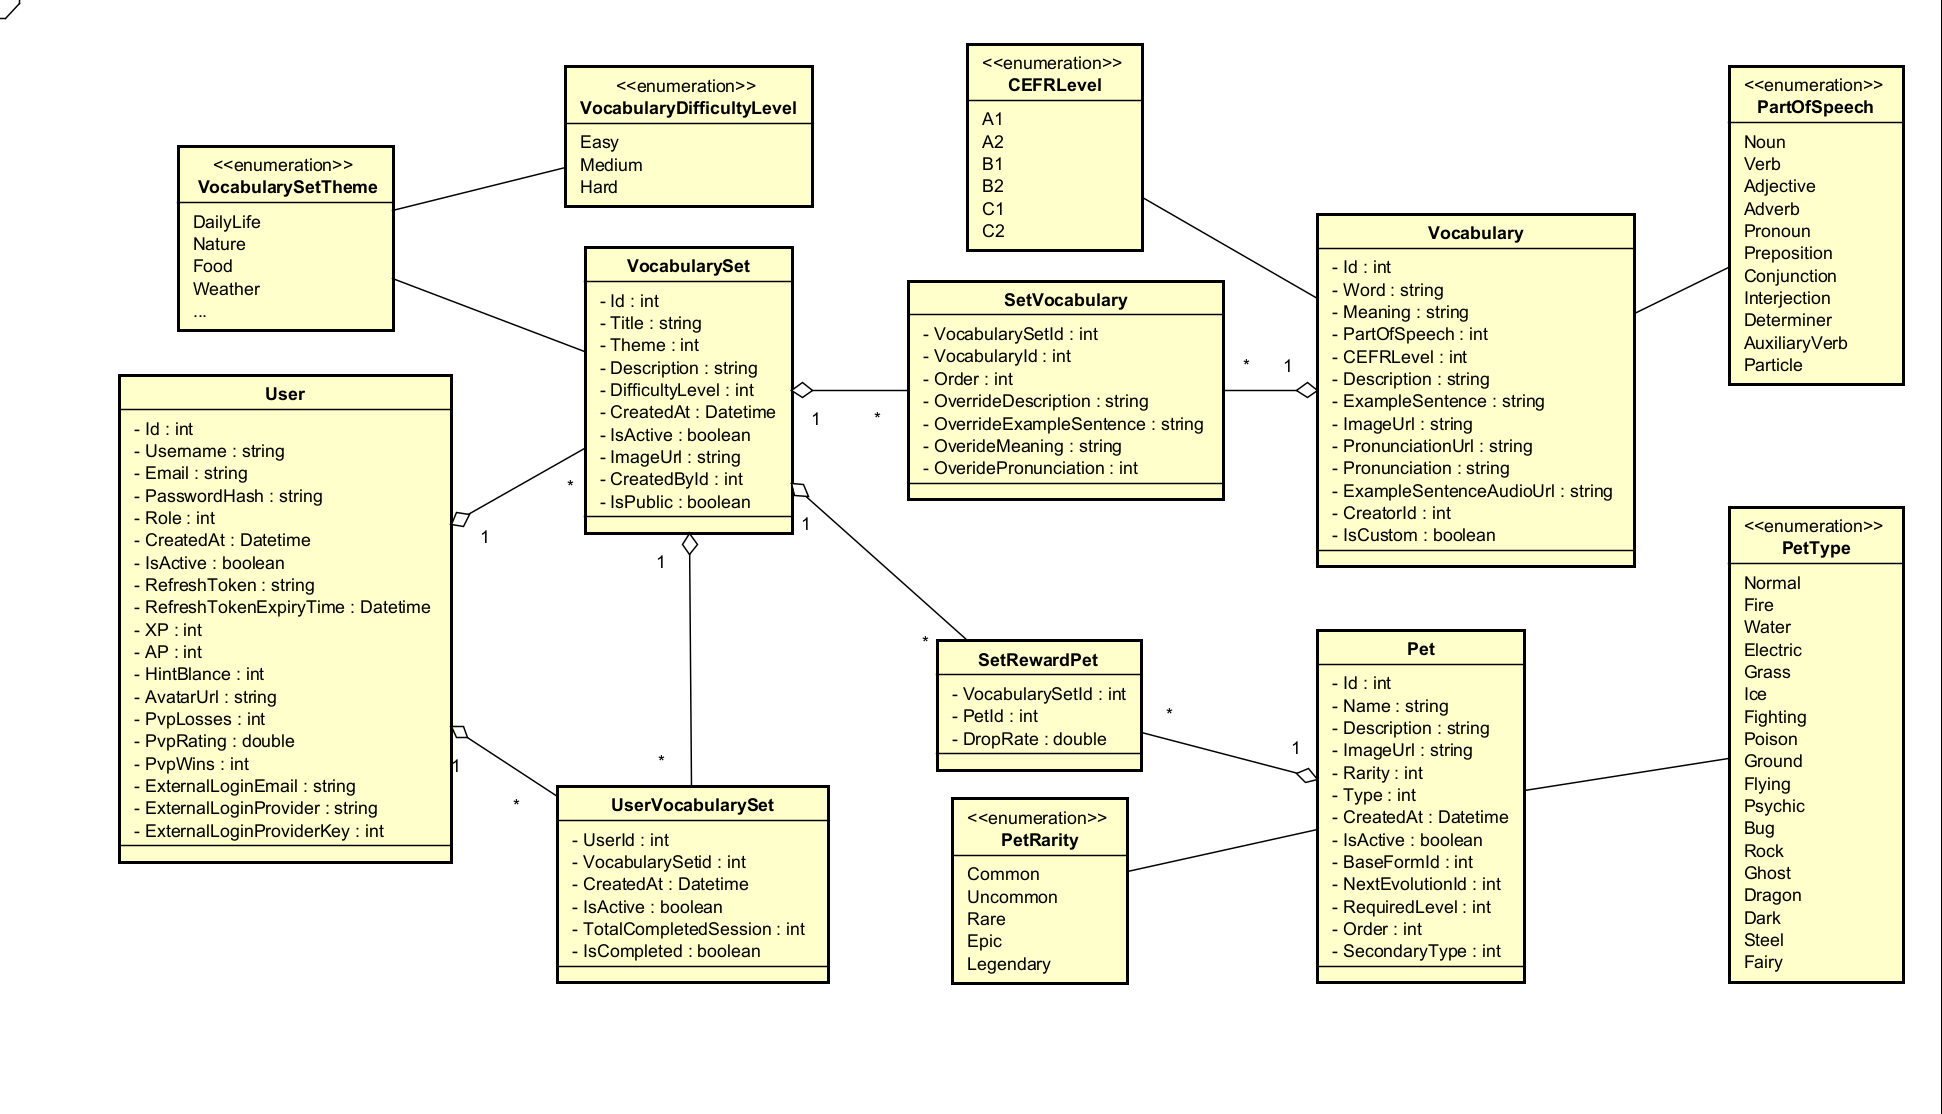
\includegraphics[width=15cm]{images/Class_Vocabulary.png}
\caption{Sơ đồ lớp nhóm Từ vựng và Nội dung học liệu.}
\label{fig_class_vocab}
\end{figure}

Thực thể \textbf{Vocabulary} lưu trữ đầy đủ thông tin ngôn ngữ học của từng đơn vị từ vựng: Word, Meaning, Pronunciation (IPA), loại từ qua enum \textbf{PartOfSpeech}, cấp độ năng lực qua enum \textbf{CEFRLevel} (A1--C2), ExampleSentence và các URL tài nguyên đa phương tiện (ImageUrl, PronunciationUrl, ExampleSentenceAudioUrl). \textbf{VocabularySet} đóng vai trò container tri thức, phân loại chủ đề qua enum \textbf{VocabularySetTheme} (19 hệ từ tương ứng PokéType) và độ khó qua enum \textbf{VocabularyDifficultyLevel} (Easy, Medium, Hard). Quan hệ nhiều-nhiều giữa VocabularySet và Vocabulary được giải quyết qua bảng trung gian \textbf{SetVocabulary}, hỗ trợ ghi đè nội dung (OverrideMeaning, OverridePronunciation) theo từng bộ từ mà không làm mất dữ liệu gốc. \textbf{UserVocabularySet} theo dõi trạng thái đăng ký và tiến độ hoàn thành (TotalCompletedSession) của người dùng với từng bộ từ. \textbf{SetRewardPet} thiết lập liên kết giữa bộ từ và thú ảo phần thưởng thông qua thuộc tính DropRate, với Pet được phân loại bởi enum \textbf{PetRarity} (Common đến Legendary) và enum \textbf{PetType} (18 hệ Pokemon).

\subsubsection{Nhóm Lịch sử học tập và Thuật toán SRS}

\begin{figure}[H]
\centering
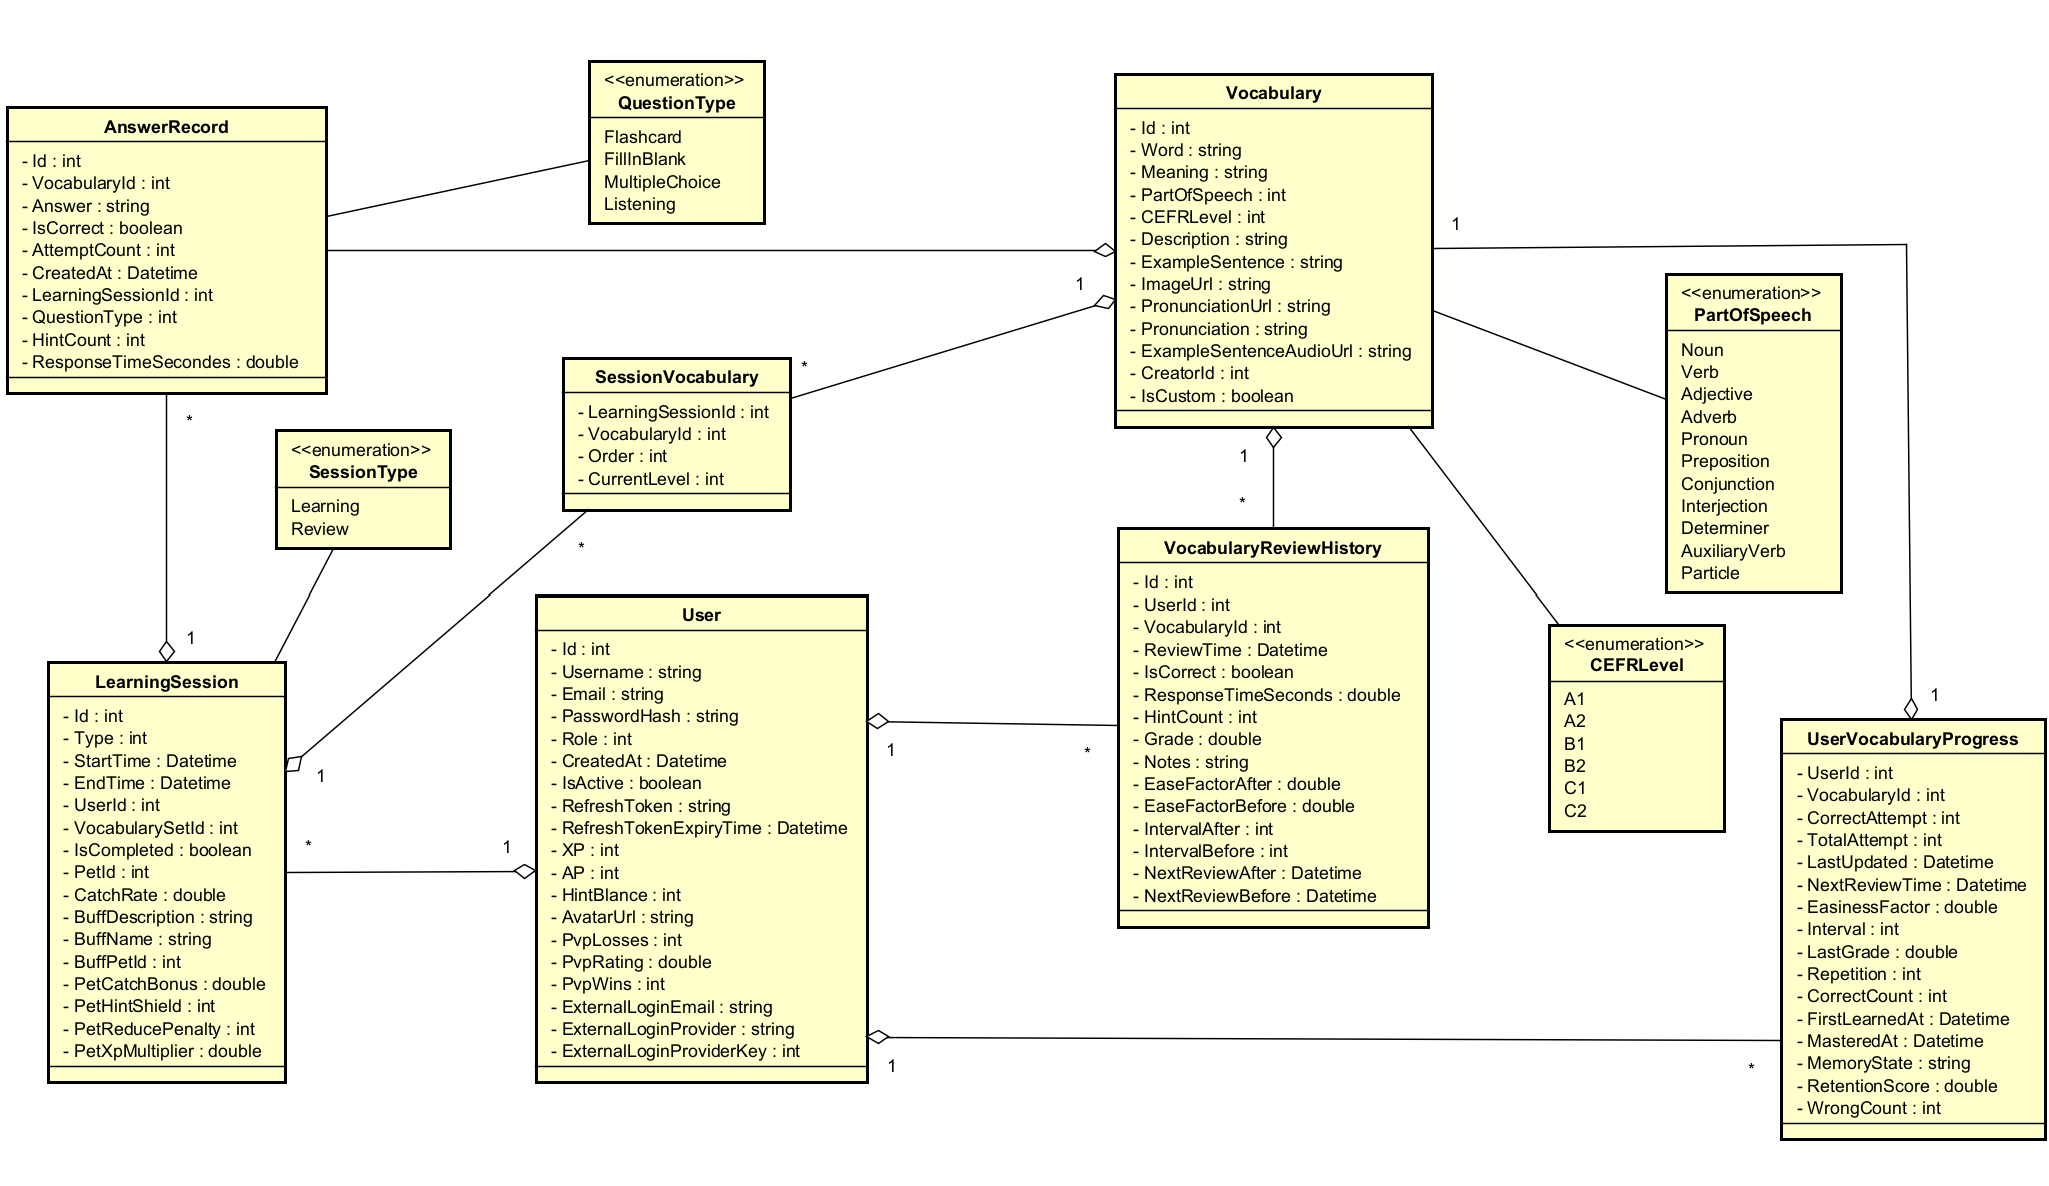
\includegraphics[width=15cm]{images/Class_Learning.png}
\caption{Sơ đồ lớp nhóm Lịch sử học tập và Thuật toán SRS.}
\label{fig_class_learning}
\end{figure}

\textbf{LearningSession} là đơn vị tổ chức phiên học, lưu loại phiên qua enum \textbf{SessionType} (Learning/Review), thông số buff từ thú ảo đang kích hoạt (PetXpMultiplier, PetCatchBonus, PetHintShield, PetReducePenalty) và xác suất bắt thú ảo (CatchRate). \textbf{SessionVocabulary} theo dõi trạng thái từng từ trong phiên qua trường CurrentLevel (0: Flashcard, 1: FillInBlank, 2: MultipleChoice, 3: Listening — tương ứng với enum \textbf{QuestionType}) và trạng thái hoàn thành. Mỗi lần trả lời được ghi vào \textbf{AnswerRecord} với IsCorrect, AttemptCount, HintCount và ResponseTimeSeconds, cung cấp nguồn dữ liệu thô cho hàm CalculateSm2Grade. Sau phiên ôn tập, \textbf{VocabularyReviewHistory} lưu nhật ký dài hạn với bộ ba trước/sau (EaseFactorBefore/After, IntervalBefore/After, NextReviewBefore/After) để phân tích xu hướng ghi nhớ. \textbf{UserVocabularyProgress} lưu trạng thái tức thời của từng cặp (User, Vocabulary): NextReviewTime, EasinessFactor, Interval, Repetition, LastGrade, MemoryState (New/Learning/Review/Mastered) và RetentionScore.

\subsubsection{Nhóm Gamification --- Thú ảo, Vật phẩm và Nhiệm vụ}

\begin{figure}[H]
\centering
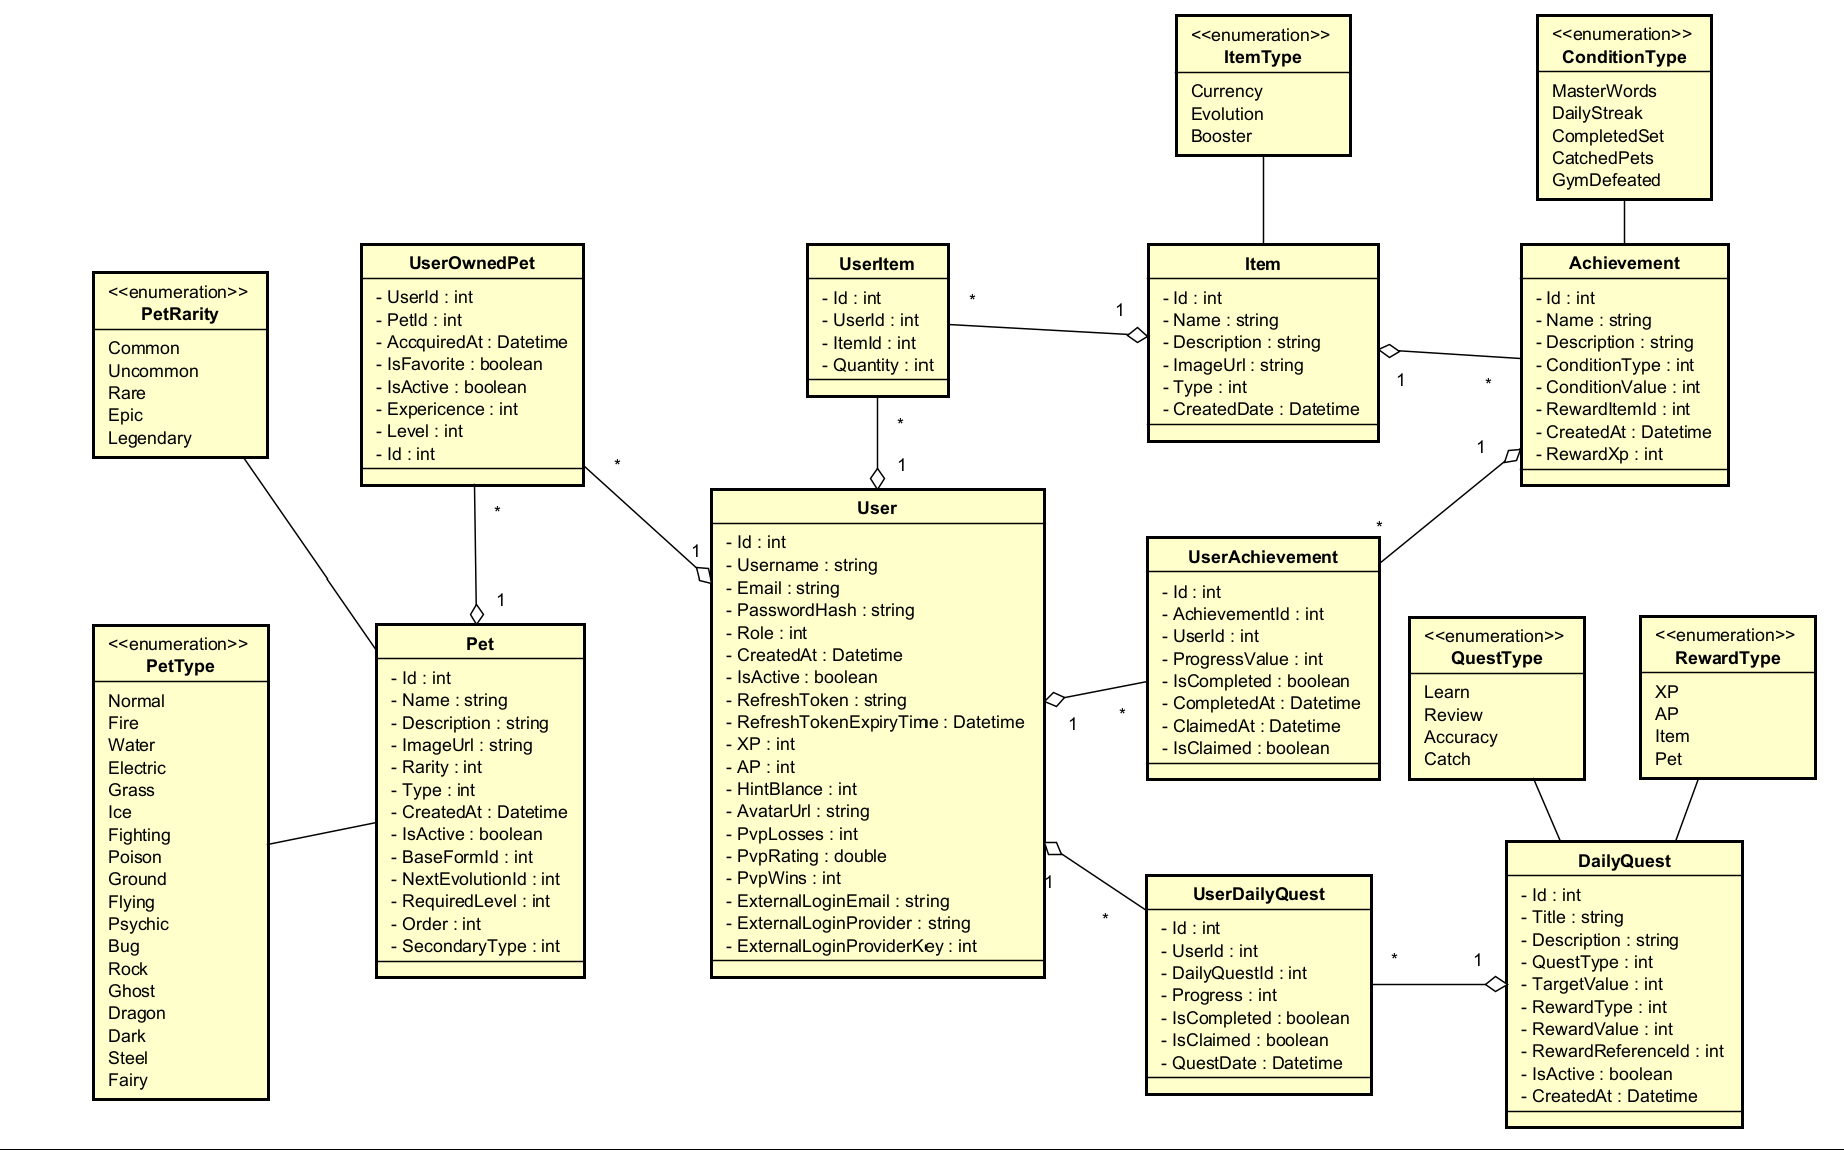
\includegraphics[width=15cm]{images/Class_Game.png}
\caption{Sơ đồ lớp nhóm Gamification --- Thú ảo, Vật phẩm và Nhiệm vụ.}
\label{fig_class_game}
\end{figure}

Thực thể \textbf{Pet} định nghĩa mẫu sinh vật ảo với Name, Rarity (enum \textbf{PetRarity}), Type/SecondaryType (enum \textbf{PetType}), chuỗi tiến hóa (BaseFormId, NextEvolutionId tự tham chiếu) và ngưỡng cấp độ tiến hóa (RequiredLevel). \textbf{UserOwnedPet} thể hiện quan hệ sở hữu của người dùng với từng thú ảo, lưu Level, Experience, trạng thái kích hoạt (IsActive) và yêu thích (IsFavorite). Vật phẩm được quản lý qua cặp \textbf{Item} (với enum \textbf{ItemType}: Currency, Evolution, Booster) và \textbf{UserItem} (Quantity). \textbf{DailyQuest} định nghĩa nhiệm vụ với loại mục tiêu (enum \textbf{QuestType}: Learn, Review, Accuracy, Catch), loại phần thưởng (enum \textbf{RewardType}: XP, AP, Item, Pet) và giá trị thưởng; \textbf{UserDailyQuest} theo dõi tiến độ (Progress), trạng thái hoàn thành và đã nhận thưởng (IsClaimed). \textbf{Achievement} định nghĩa thành tích dài hạn với điều kiện mở khóa qua enum \textbf{ConditionType} (MasterWords, DailyStreak, CompletedSet, CatchedPets, GymDefeated); \textbf{UserAchievement} lưu ProgressValue, IsCompleted và ClaimedAt.

\subsubsection{Nhóm Hệ thống Đối kháng}

\begin{figure}[H]
\centering
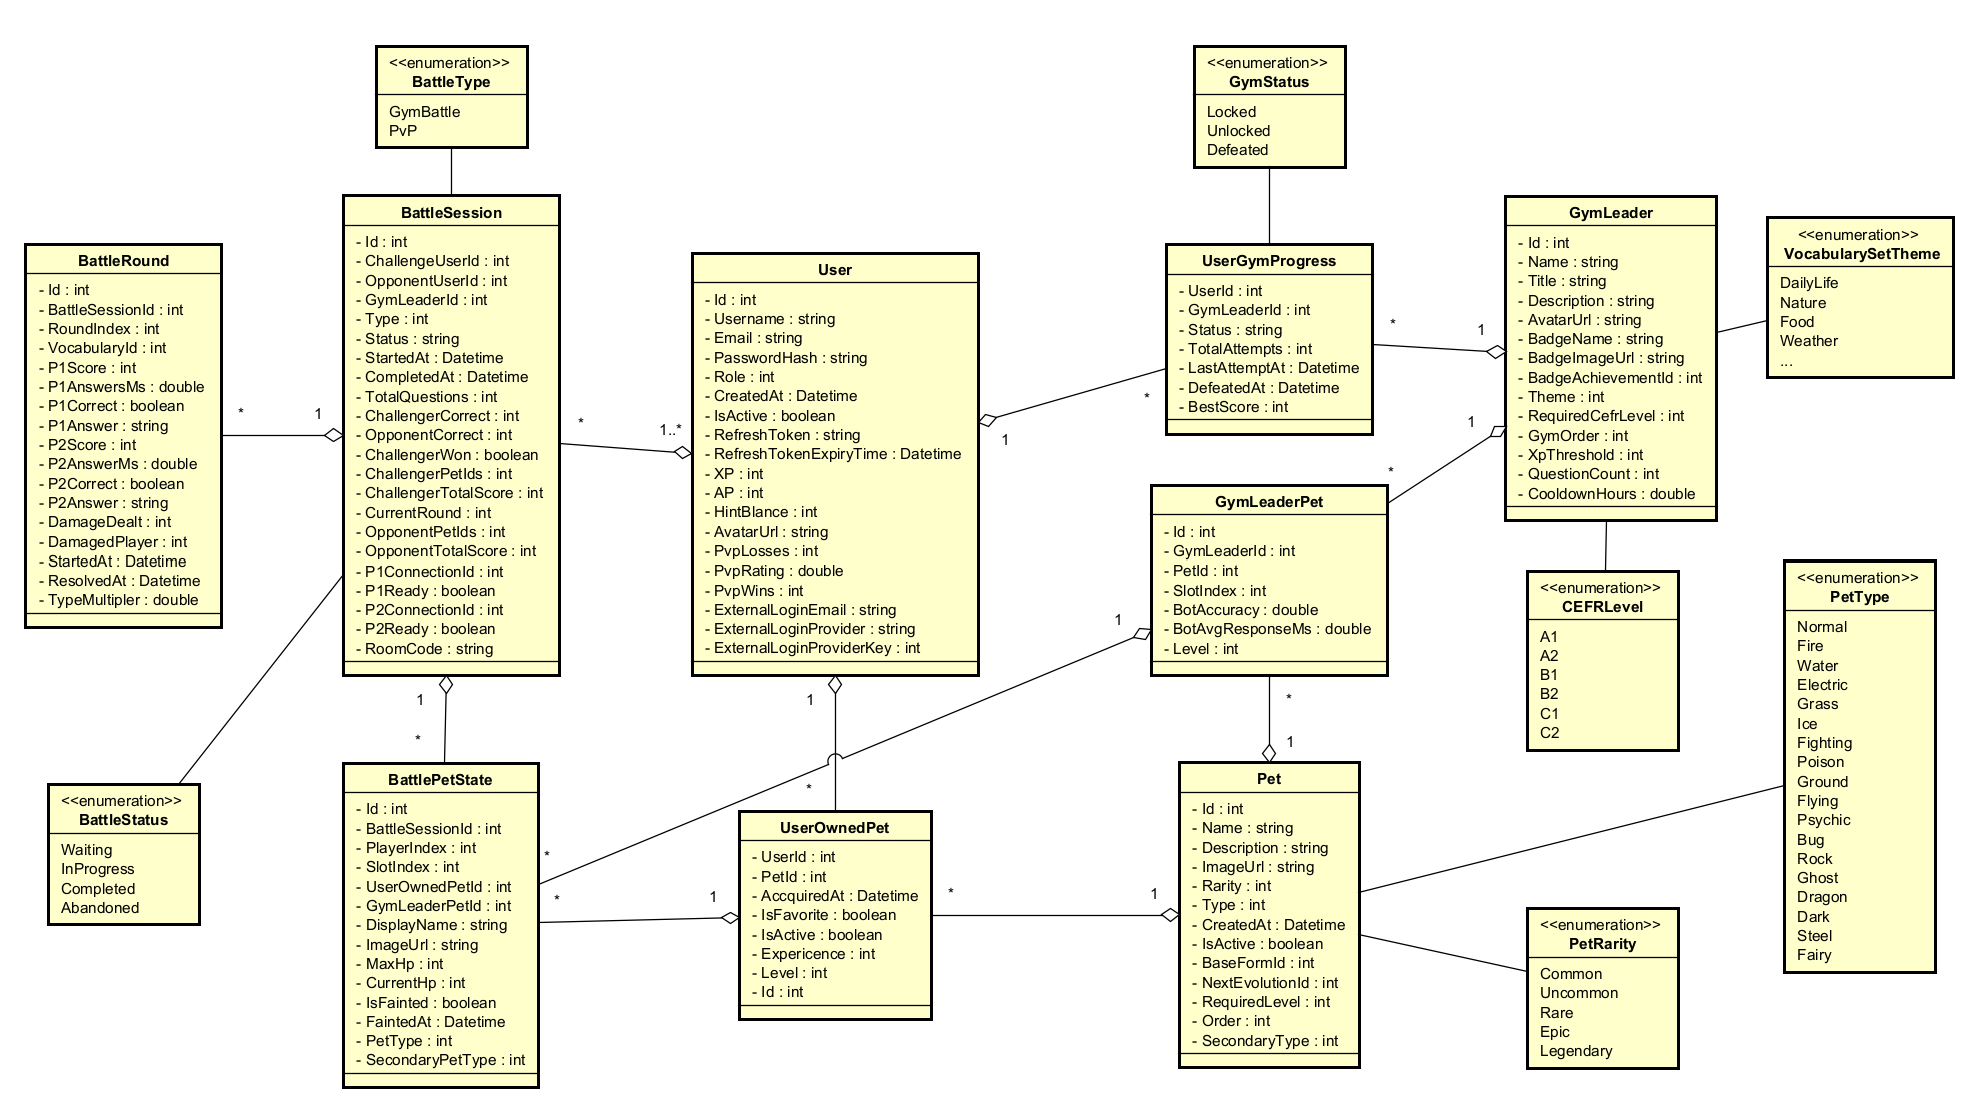
\includegraphics[width=15cm]{images/Class_Battle.png}
\caption{Sơ đồ lớp nhóm Hệ thống Đối kháng.}
\label{fig_class_battle}
\end{figure}

\textbf{BattleSession} quản lý một phiên đấu đầy đủ, lưu thông tin hai phía Challenger/Opponent (UserId, điểm số, trạng thái kết nối SignalR, danh sách ID thú ảo tham chiến), phân loại trạng thái qua enum \textbf{BattleStatus} (Waiting, Abandoned). \textbf{BattleRound} ghi nhận kết quả từng câu hỏi: điểm số P1/P2, thời gian phản hồi (P1AnswerMs, P2AnswerMs), tính đúng/sai và hệ số nhân sát thương TypeMultiplier theo ma trận khắc chế thuộc tính PetType. \textbf{BattlePetState} duy trì HP (MaxHp, CurrentHp) và trạng thái sống còn (IsFainted, FaintedAt) của từng thú ảo trong phiên, cho phép phục hồi trạng thái nếu kết nối WebSocket bị gián đoạn. Đối với chế độ PvE, \textbf{GymLeader} định nghĩa Gym Boss với ngưỡng mở khóa (XpThreshold, VocabThreshold), thông số trận đấu (QuestionCount, CooldownHours) và phần thưởng (XpReward, BadgeAchievementId); \textbf{GymLeaderPet} định nghĩa đội hình kèm tham số bot AI (BotAccuracy, BotAvgResponseMs, Level). \textbf{UserGymProgress} theo dõi tiến độ chinh phục từng Gym qua enum \textbf{GymStatus} (Locked, Unlocked, Defeated), lưu TotalAttempts, BestScore và thời điểm đánh bại (DefeatedAt).

\subsection{Thiết kế mô hình dữ liệu vật lý}

Lược đồ cơ sở dữ liệu vật lý là bản hiện thực hóa các thực thể logic thành các cấu trúc lưu trữ cụ thể trên hệ quản trị SQL Server. Kiến trúc này được thiết kế với mục tiêu tối thượng là bảo toàn tính toàn vẹn dữ liệu thông qua mạng lưới khóa chính (PK) và khóa ngoại (FK) chặt chẽ, đồng thời tạo ra một cấu trúc tối ưu cho các tác vụ truy xuất lịch sử học tập và điều phối dữ liệu trận đấu thời gian thực với độ trễ thấp nhất.

Nhằm đảm bảo tính dễ đọc khi in ấn và phục vụ cho việc tra cứu chi tiết cột, kiểu dữ liệu và ràng buộc khóa ngoại, lược đồ cơ sở dữ liệu vật lý được phân rã thành năm nhóm sub-diagram độc lập theo phạm vi nghiệp vụ tương ứng.

\subsubsection{Nhóm Quản lý người dùng và Xác thực}

\begin{figure}[H]
\centering
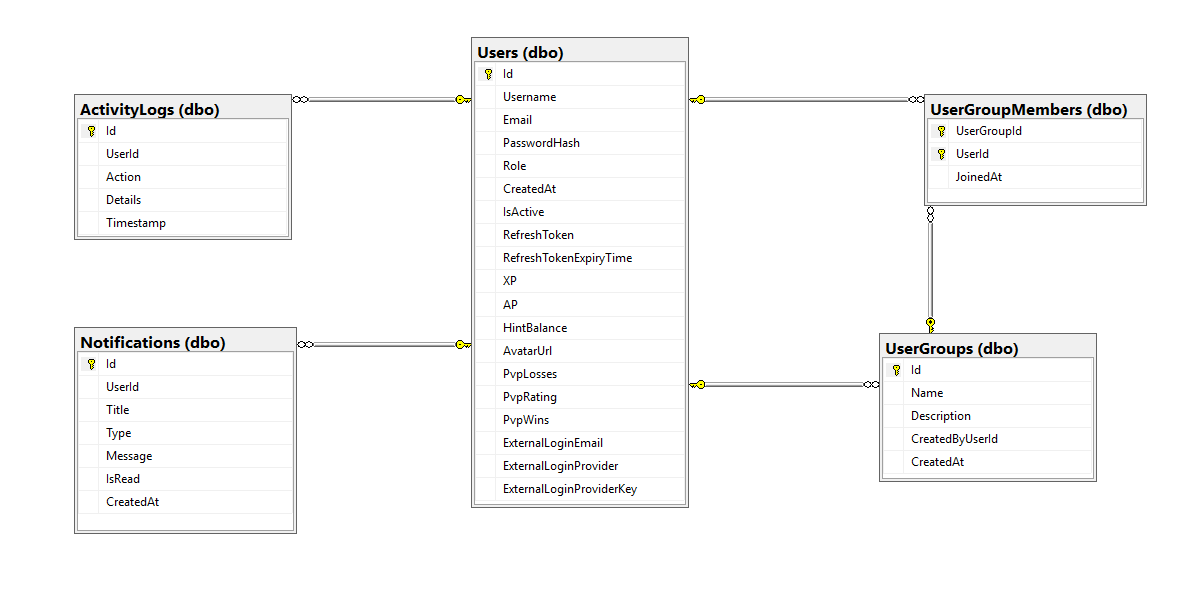
\includegraphics[width=14cm]{images/Db_User.png}
\caption{Lược đồ ERD nhóm Quản lý người dùng và Xác thực.}
\label{fig_erd_users}
\end{figure}

Bảng \textbf{Users} là điểm hội tụ trung tâm, lưu thông tin xác thực (Email, PasswordHash, RefreshToken, RefreshTokenExpiryTime), hồ sơ cá nhân (Username, AvatarUrl) và các chỉ số vận hành (XP, AP, PvpRating, PvpWins, PvpLosses, IsActive). Bảng \textbf{ActivityLogs} ghi nhật ký hoạt động với Timestamp, liên kết FK tới Users. Bảng \textbf{UserGroups} định nghĩa nhóm học tập (Name, Description, CreatedByUserId); bảng \textbf{UserGroupMembers} là bảng trung gian nhiều-nhiều giữa Users và UserGroups, ghi nhận JoinedAt. Bảng \textbf{Notifications} phân loại thông báo đẩy qua cột Type (enum NotificationType: Review, Reward, Event), liên kết FK tới Users với ràng buộc Cascade Delete đảm bảo tính toàn vẹn khi xóa tài khoản.

\subsubsection{Nhóm Từ vựng và Nội dung học liệu}

\begin{figure}[H]
\centering
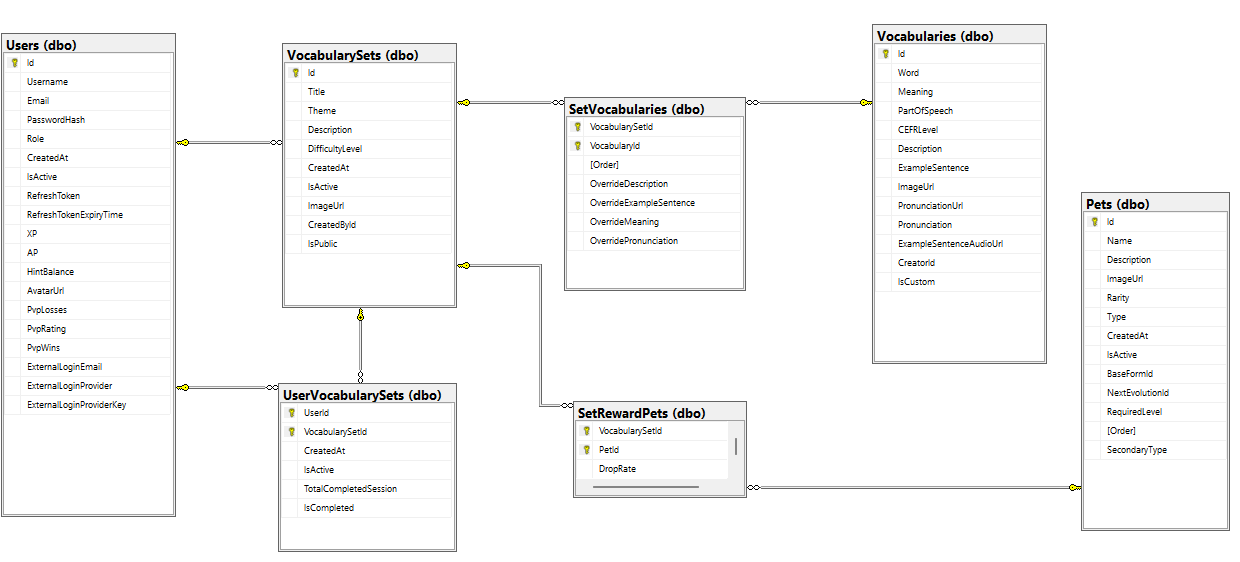
\includegraphics[width=14cm]{images/Db_Vocabulary.png}
\caption{Lược đồ ERD nhóm Từ vựng và Nội dung học liệu.}
\label{fig_erd_vocab}
\end{figure}

Bảng \textbf{Vocabularies} lưu đầy đủ thông tin ngôn ngữ học: Word, Meaning, Pronunciation (IPA), PartOfSpeech, CEFRLevel, ExampleSentence, ImageUrl, PronunciationUrl, ExampleSentenceAudioUrl (Azure TTS) cùng cờ IsCustom và CreatorId. Bảng \textbf{VocabularySets} định nghĩa bộ từ với Title, Theme (VocabularySetTheme), DifficultyLevel (VocabularyDifficultyLevel), IsPublic và CreatedById (FK tới Users). Quan hệ nhiều-nhiều được giải quyết qua bảng trung gian \textbf{SetVocabularies} với PK kép (VocabularySetId, VocabularyId), hỗ trợ ghi đè nội dung (OverrideMeaning, OverridePronunciation, OverrideExampleSentence) theo từng bộ mà không làm mất dữ liệu gốc. Bảng \textbf{UserVocabularySets} ghi nhận đăng ký của người dùng với TotalCompletedSession — thông số điều phối xác suất phần thưởng thú ảo hiếm theo cơ chế leo thang. Bảng \textbf{SetRewardPets} (PK kép: VocabularySetId, PetId) thiết lập tỉ lệ rơi đồ (DropRate) cho từng thú ảo phần thưởng gắn với bộ từ.

\subsubsection{Nhóm Lịch sử học tập và Thuật toán SRS}

\begin{figure}[H]
\centering
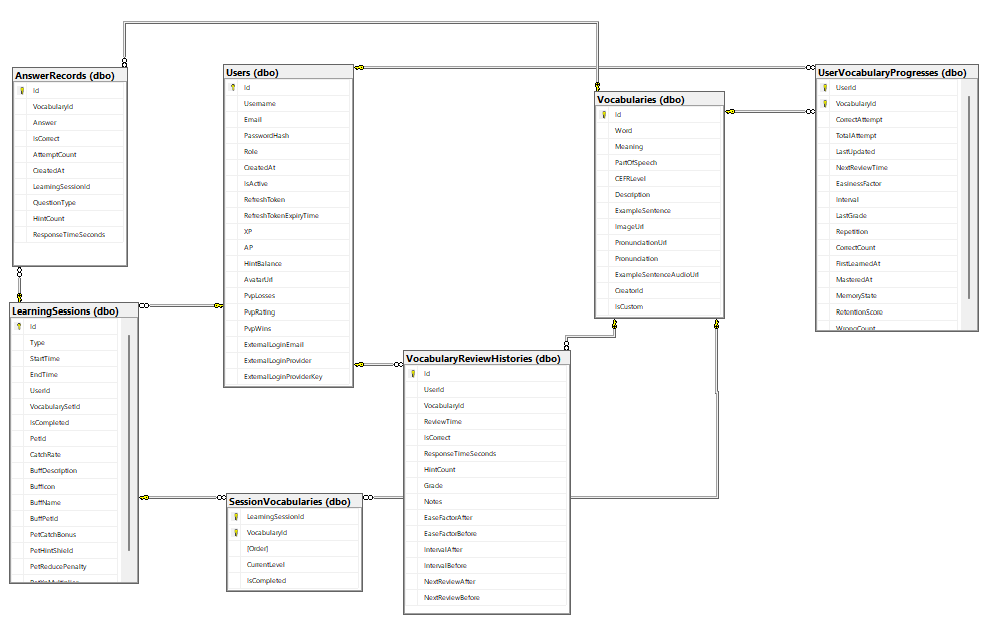
\includegraphics[width=14cm]{images/Db_Learning.png}
\caption{Lược đồ ERD nhóm Lịch sử học tập và Thuật toán SRS.}
\label{fig_erd_srs}
\end{figure}

Bảng \textbf{LearningSessions} tổ chức phiên học với SessionType (Learning/Review), thời gian bắt đầu/kết thúc, FK tới VocabularySetId, PetId (thú ảo phần thưởng) và các thông số buff (PetXpMultiplier, PetCatchBonus, PetHintShield, PetReducePenalty, CatchRate). Bảng \textbf{SessionVocabularies} (PK kép: LearningSessionId, VocabularyId) theo dõi từng từ trong phiên với CurrentLevel (0--3 tương ứng QuestionType: Flashcard, FillInBlank, MultipleChoice, Listening) và IsCompleted. Bảng \textbf{AnswerRecords} ghi nhận từng lần trả lời với IsCorrect, AttemptCount, HintCount, ResponseTimeSeconds — dữ liệu thô cho hàm CalculateSm2Grade. Hai bảng cốt lõi cho thuật toán SM-2: \textbf{UserVocabularyProgresses} (PK kép: UserId, VocabularyId) lưu trạng thái tức thời gồm EasinessFactor, Interval, Repetition, LastGrade, NextReviewTime, MemoryState và RetentionScore; \textbf{VocabularyReviewHistories} lưu nhật ký mỗi lần ôn tập với bộ giá trị trước/sau (EaseFactorBefore/After, IntervalBefore/After, NextReviewBefore/After) phục vụ phân tích xu hướng quên lãng dài hạn.

\subsubsection{Nhóm Gamification --- Thú ảo, Vật phẩm và Nhiệm vụ}

\begin{figure}[H]
\centering
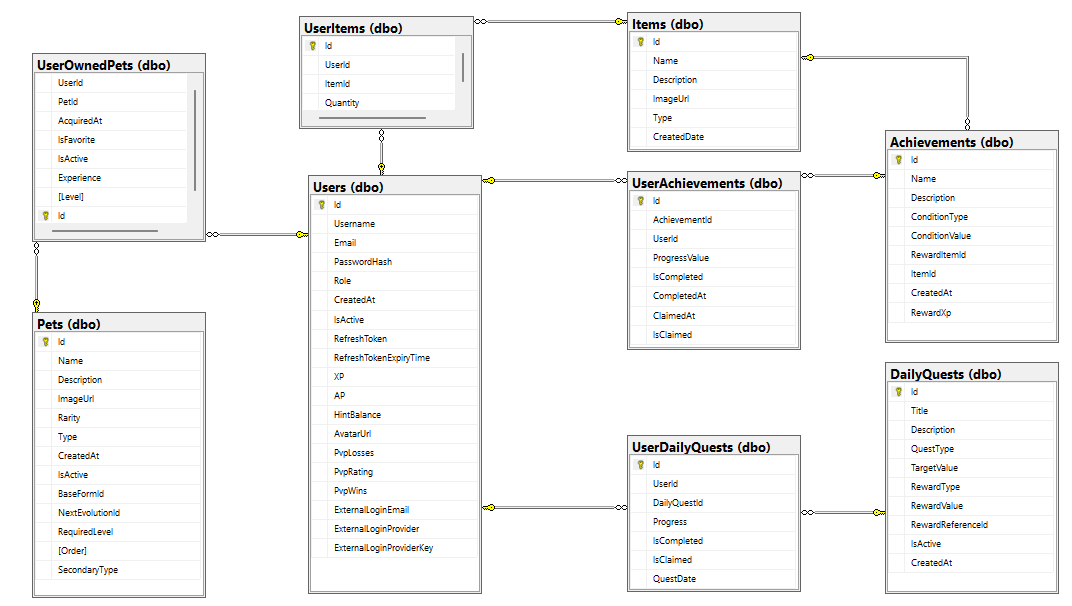
\includegraphics[width=14cm]{images/Db_Game.png}
\caption{Lược đồ ERD nhóm Gamification --- Thú ảo, Vật phẩm và Nhiệm vụ.}
\label{fig_erd_gamification}
\end{figure}

Bảng \textbf{Pets} định nghĩa mẫu sinh vật ảo với Name, Rarity (PetRarity), Type/SecondaryType (PetType), chuỗi tiến hóa tự tham chiếu (BaseFormId, NextEvolutionId), RequiredLevel và ImageUrl. Bảng \textbf{UserOwnedPets} thể hiện quan hệ sở hữu với Level, Experience, IsActive, IsFavorite và AcquiredAt. Hệ thống vật phẩm gồm \textbf{Items} (Name, Description, ItemType: Currency/Evolution/Booster) và \textbf{UserItems} (UserId, ItemId, Quantity) với ràng buộc duy nhất trên cặp (UserId, ItemId) đảm bảo tính nhất quán tồn kho. Bảng \textbf{DailyQuests} định nghĩa nhiệm vụ với QuestType, RewardType, TargetValue, RewardValue, RewardReferenceId; \textbf{UserDailyQuests} theo dõi Progress, IsCompleted, IsClaimed và QuestDate. Bảng \textbf{Achievements} lưu điều kiện mở khóa (ConditionType, ConditionValue) và phần thưởng (RewardXp, RewardItemId); \textbf{UserAchievements} theo dõi ProgressValue, IsCompleted, CompletedAt và IsClaimed.

\subsubsection{Nhóm Hệ thống Đối kháng}

\begin{figure}[H]
\centering
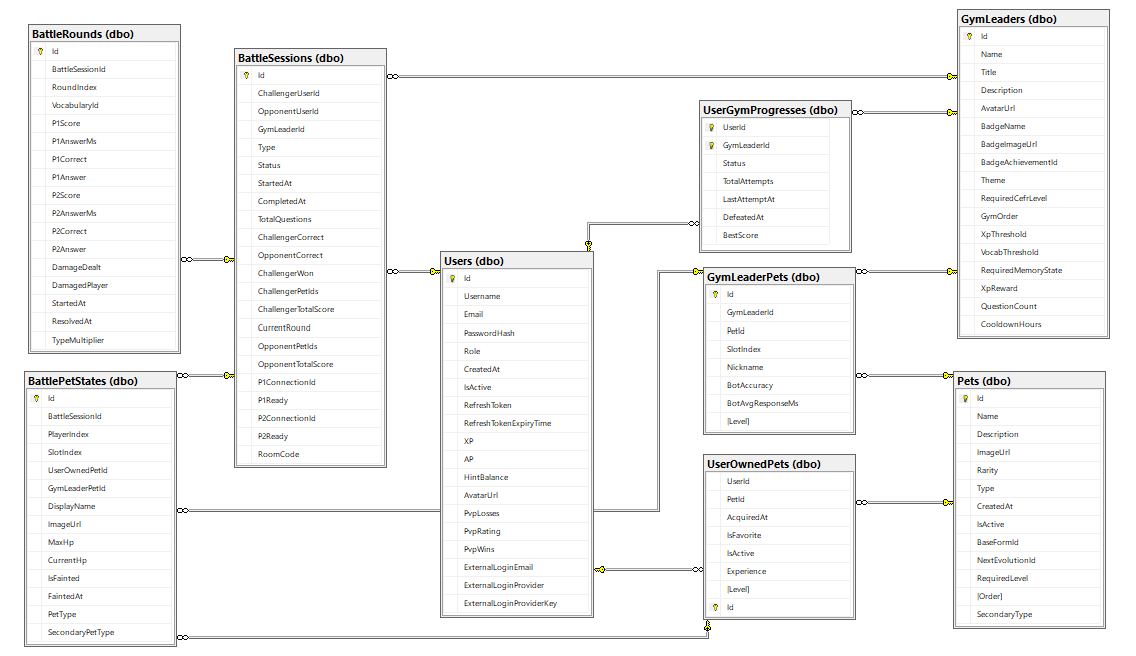
\includegraphics[width=14cm]{images/Db_Battle.png}
\caption{Lược đồ ERD nhóm Hệ thống Đối kháng.}
\label{fig_erd_battle}
\end{figure}

Bảng \textbf{BattleSessions} lưu toàn bộ thông tin một phiên đấu: ChallengerUserId, OpponentUserId (PvP) hoặc GymLeaderId (PvE), điểm số hai phía (ChallengerTotalScore, OpponentTotalScore), tín hiệu sẵn sàng (P1Ready, P2Ready), ConnectionId SignalR và ChallengerWon (null = chưa kết thúc). Bảng \textbf{BattleRounds} ghi kết quả từng câu hỏi: VocabularyId, điểm số P1/P2 (P1Score, P2Score), thời gian phản hồi (P1AnswerMs, P2AnswerMs), tính đúng/sai và TypeMultiplier theo ma trận khắc chế thuộc tính PetType. Bảng \textbf{BattlePetStates} duy trì HP (MaxHp, CurrentHp), IsFainted và FaintedAt cho từng thú ảo (UserOwnedPetId hoặc GymLeaderPetId), đảm bảo khả năng phục hồi kết nối WebSocket. Đối với chế độ PvE, \textbf{GymLeaders} lưu ngưỡng mở khóa (XpThreshold, VocabThreshold, RequiredMemoryState), thông số trận đấu (QuestionCount, CooldownHours) và phần thưởng; \textbf{GymLeaderPets} định nghĩa đội hình của Gym Boss kèm tham số bot AI (BotAccuracy, BotAvgResponseMs). Bảng \textbf{UserGymProgresses} (PK kép: UserId, GymLeaderId) theo dõi GymStatus (Locked/Unlocked/Defeated), TotalAttempts, BestScore và DefeatedAt.

Tổng thể lược đồ này không chỉ đáp ứng các tiêu chuẩn lưu trữ hiện hành mà còn thiết lập một nền tảng dữ liệu sạch, sẵn sàng cho các bài toán phân tích chuyên sâu hoặc mở rộng tính năng xã hội trong tương lai.

\newpage
\section{Thiết kế giao diện người dùng và Trải nghiệm người dùng}
\subsection{Giao diện Bảng vinh danh cộng đồng}
Nhằm tối ưu hóa tính cộng đồng, giao diện Bảng vinh danh được thiết kế theo hướng minh bạch hóa kết quả, lấy điểm tích lũy làm thước đo để thúc đẩy sự thi đua lành mạnh giữa các cá nhân trong hệ thống.

\begin{figure}[H]
\centering
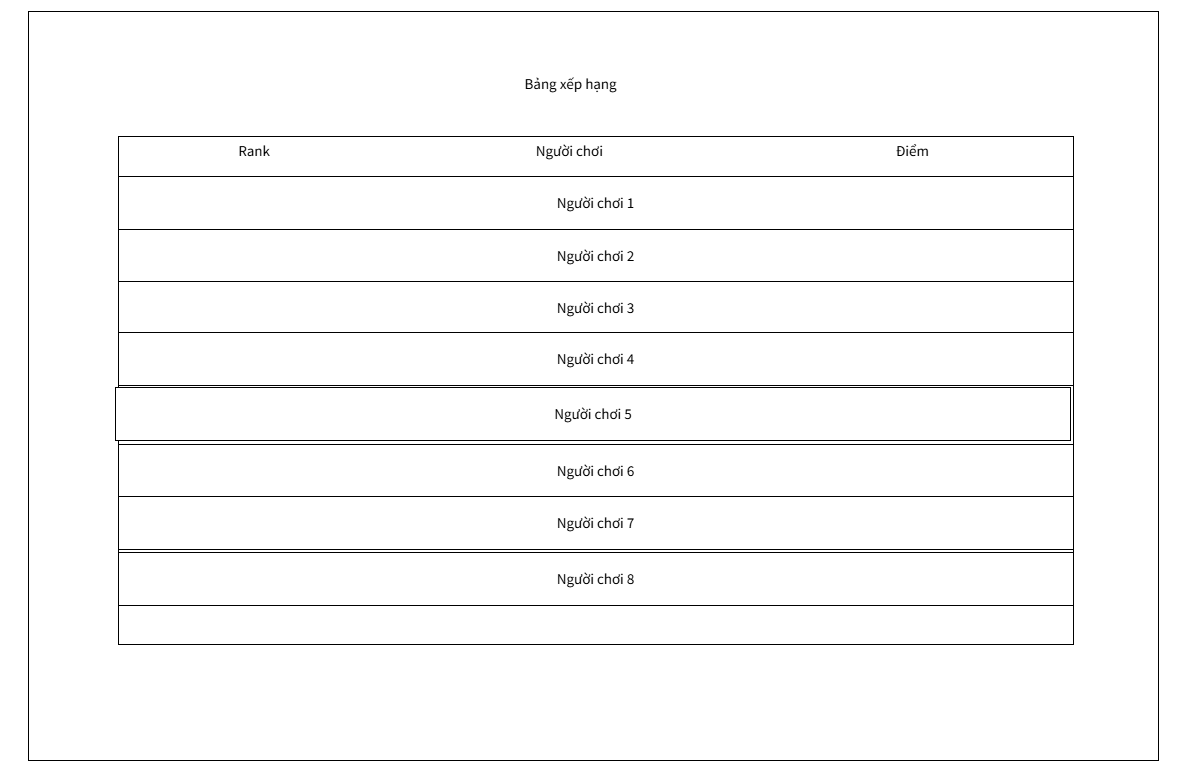
\includegraphics[width=15cm]{images/Bxh.png}
\caption{Thiết kế giao diện hệ thống xếp hạng cộng đồng.}
\label{fig:ch3_leaderboard}
\end{figure}

\subsection{Cơ chế quản trị học liệu đa tầng}

Hệ thống sở hữu một môi trường quản lý kho từ vựng linh hoạt, hỗ trợ tối đa việc cá nhân hóa kiến thức thông qua các bộ lọc thông minh. Quy trình kiến tạo bộ học liệu được triển khai theo một tiến trình logic hai giai đoạn: xác lập đơn vị tri thức và cấu trúc hóa dữ liệu (bao gồm nhận diện chủ đề và định vị ngưỡng thử thách). Màn hình chi tiết được thiết kế để trực quan hóa tiến trình ghi nhớ của từng mục từ, giúp người học nhận diện rõ ràng những mảng kiến thức đã làm chủ và những phần cần đầu tư thêm nỗ lực.

\begin{figure}[H]
\centering
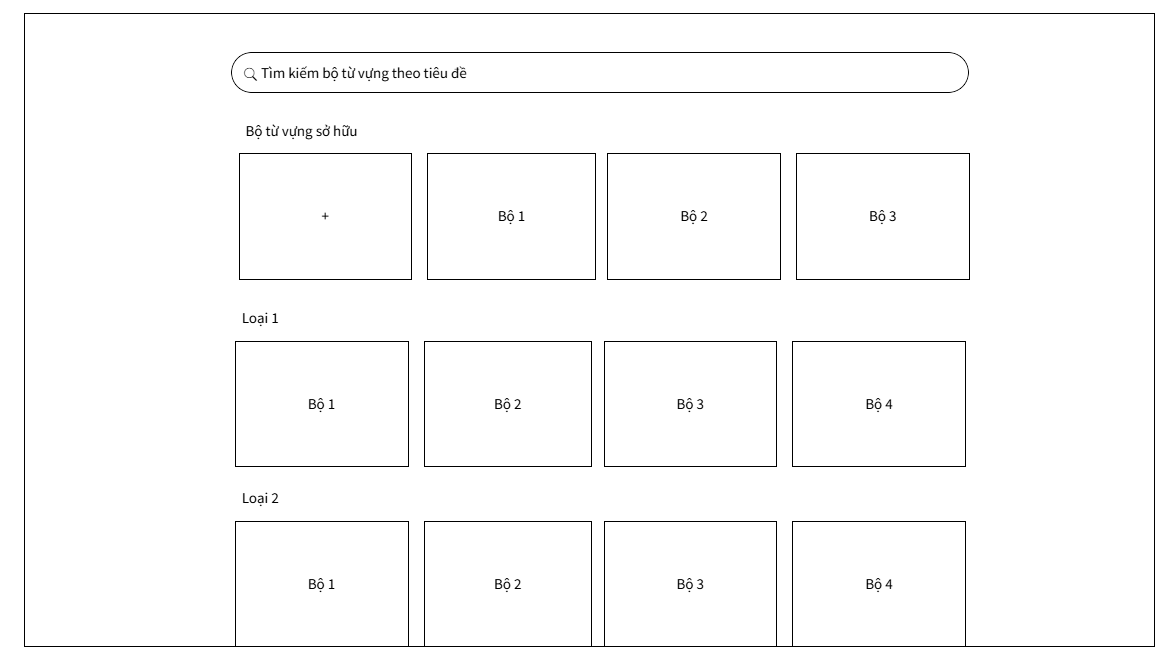
\includegraphics[width=15cm]{images/Sets.png}
\caption{Cấu trúc thiết kế quản lý danh mục bộ học liệu.}
\label{fig:ch3_sets}
\end{figure}

\subsection{Không gian tương tác và Gắn kết cảm xúc}

Giao diện thú ảo là nhân tố then chốt trong việc duy trì sợi dây liên kết cảm xúc giữa người dùng và ứng dụng. Hệ thống cung cấp các màng lọc nâng cao dựa trên thuộc tính nguyên tố và mức độ quý hiếm, giúp việc quản lý bộ sưu tập cá nhân trở nên trực quan hơn. Tại đây, mọi thông số từ cấp độ tiến hóa đến năng lực chiến đấu được trình bày sinh động, kích thích khao khát đầu tư công sức học tập để chứng kiến sự trưởng thành của sinh vật đồng hành.

\begin{figure}[H]
\centering
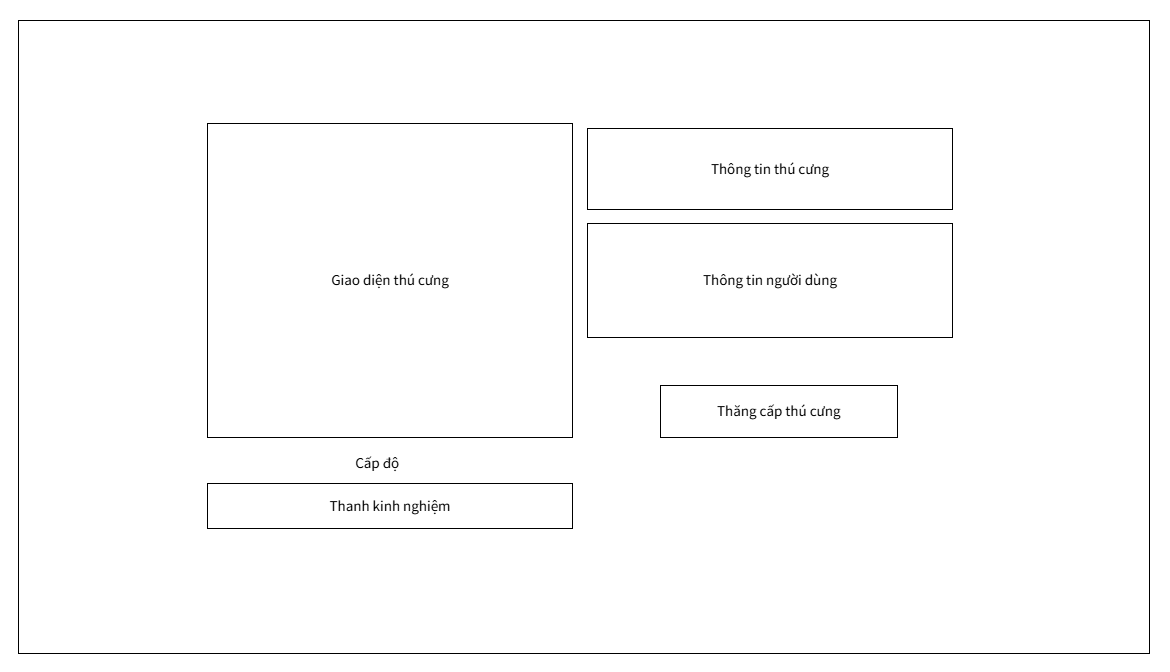
\includegraphics[width=13cm]{images/Pet.png}
\caption{Chi tiết thiết kế giao diện phát triển sinh vật ảo.}
\label{fig:ch3_pet_detail}
\end{figure}

\subsection{Tối ưu hóa trải nghiệm tiếp nhận tri thức}

Triết lý thiết kế của các phiên tương tác kiến thức được điều chỉnh linh hoạt theo mục đích tâm lý học. Giao diện Ôn tập tận dụng các yếu tố đồ họa động và phản hồi tức thì — như hiệu ứng chăm sóc Pet khi đưa ra đáp án đúng — để duy trì trạng thái hưng phấn \cite{Hamari2014}. Ngược lại, không gian Học mới được tinh giản theo phong cách Minimalism, loại bỏ mọi tác nhân gây nhiễu để người dùng đạt được trạng thái tập trung cao độ khi tiếp cận các khái niệm mới \cite{Bjork2011}. Cả hai mô hình đều được trang bị thanh tiến độ thời gian thực, giúp người học định vị chính xác vị trí của mình trong mỗi phiên làm việc.

\begin{figure}[H]
\centering
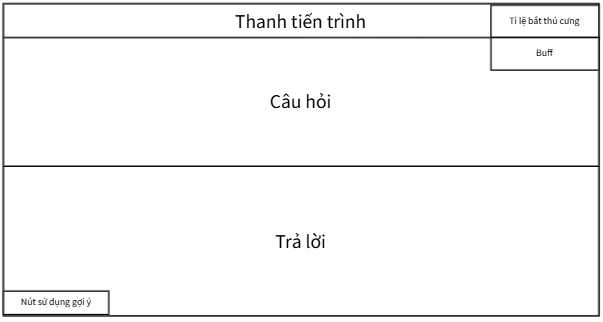
\includegraphics[width=12cm]{images/Learn.png}
\caption{Thiết kế giao diện chu trình học tập và củng cố kiến thức.}
\label{fig:ch3_learn_flow}
\end{figure}

\subsection{Nhóm Đối kháng}

Phân hệ đối kháng được thiết kế để chuyển hóa việc kiểm tra kiến thức thành một trải nghiệm giải trí cạnh tranh cao. Ở chế độ PvE, giao diện thách đấu Gym Leader tái hiện lộ trình chinh phục thử thách theo từng cấp bậc thành tựu. Trong khi đó, chế độ PvP cung cấp không gian sảnh chờ chuyên nghiệp với chỉ số Elo và các tính năng tạo phòng linh hoạt. Giao diện đối kháng chung được thiết kế để ưu tiên tốc độ và độ chính xác, nơi các câu hỏi trắc nghiệm trở thành công cụ quyết định thắng bại trong môi trường thời gian thực \cite{Deterding2011}.

\begin{figure}[H]
\centering
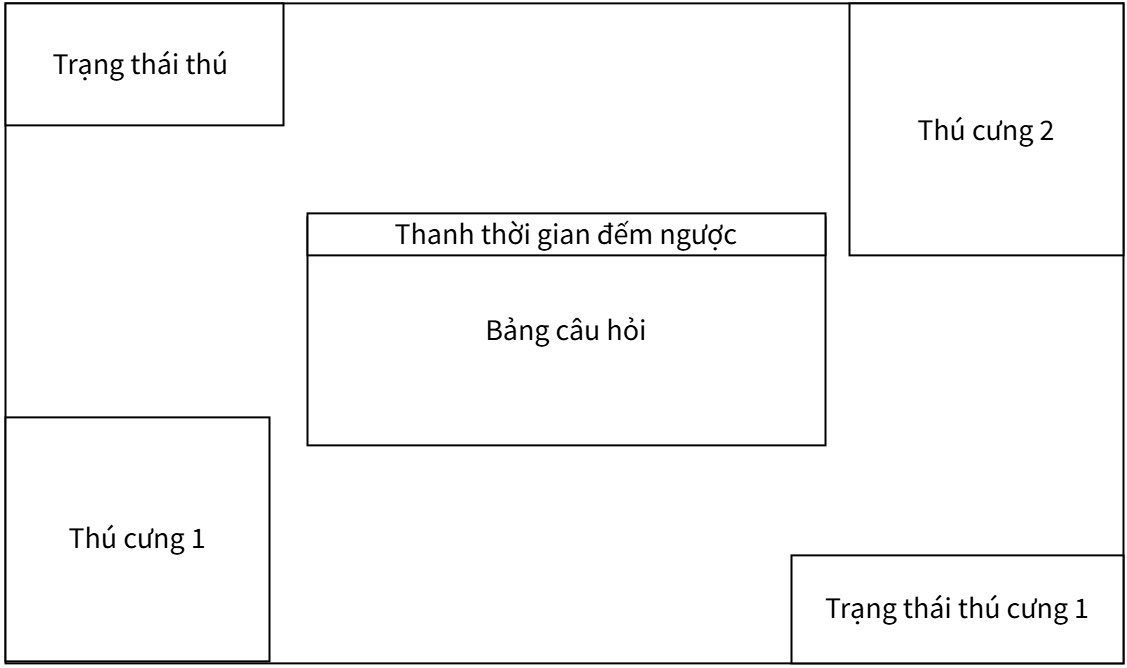
\includegraphics[width=11cm]{images/Mock_Pvp.png}
\caption{Thiết kế giao diện Chiến đấu thời gian thực}
\label{fig:ch3_battle}
\end{figure}

Tổng thể bộ giao diện đã bao quát toàn diện các kịch bản sử dụng quan trọng, đảm bảo tính khả thi cao khi triển khai kỹ thuật. Bố cục trực quan phối hợp cùng các cơ chế phản hồi tức thì tạo nên một hệ thống không chỉ mạnh mẽ về chức năng mà còn hấp dẫn về mặt trải nghiệm, góp phần duy trì thói quen học tập bền vững cho người dùng.


\section{Đánh giá kết quả thực thi dự án}

Sau chu trình khép kín từ phân tích, thiết kế đến thực thi kỹ thuật, hệ thống đã hoàn tất việc chuyển đổi các mục tiêu nghiên cứu thành một giải pháp phần mềm có tính ứng dụng cao. Kết quả đạt được ghi nhận sự tương thích tuyệt đối giữa các module nghiệp vụ phức hợp với hệ thống yêu cầu chức năng đã xác lập ban đầu. Không dừng lại ở các mô hình lý thuyết, sản phẩm hiện tại đã đạt tới trạng thái sẵn sàng cho các kịch bản triển khai thực tế trên diện rộng, đánh dấu sự thành công trong việc tích hợp các quy tắc Gamification vào một nền tảng học thuật chính thống.

Sự vận hành đồng bộ giữa các phân hệ — từ thuật toán lặp lại ngắt quãng, cơ chế đối kháng thời gian thực đến hệ sinh thái thú ảo — đã minh chứng cho tính đúng đắn của việc lựa chọn kiến trúc hành tây (Onion Architecture) kết hợp cùng hệ sinh thái .NET 8 và ReactJS. Những kết quả thực thi này không chỉ phản ánh năng lực xử lý dữ liệu ổn định mà còn cho thấy sự tối ưu hóa trong trải nghiệm người dùng (UX), kiến tạo nên một môi trường học tập trực quan, sinh động và có khả năng duy trì động lực bền vững.

\subsection{Cơ chế vận hành phiên học và củng cố tri thức}

Hệ thống đã triển khai một quy trình tiếp nhận tri thức dựa trên sự giao thoa chiến lược giữa hai nguyên lý khoa học nhận thức là lặp lại ngắt quãng và thực hành truy hồi chủ động (Active Recall). Bằng việc triển khai thuật toán SM-2 tiêu chuẩn kết hợp hàm chấm điểm đa yếu tố tự động (hàm CalculateSm2Grade, trình bày chi tiết ở phần sau), dự án cho phép thiết lập các phiên tương tác cá nhân hóa, nơi các thuật toán phân tích sẽ ưu tiên truy xuất những đơn vị ngôn ngữ có chỉ số ghi nhớ thấp hoặc thường xuyên gây nhầm lẫn trong lịch sử học tập. Phương thức tiếp cận này giúp tối ưu hóa hiệu suất nhận thức bằng cách tập trung cường độ rèn luyện vào các vùng kiến thức chưa vững chắc, thay vì lãng phí tài nguyên thời gian cho những nội dung đã đạt ngưỡng thành thạo.

Không gian tương tác trong mỗi phiên học được xây dựng theo hướng trực quan hóa, kết hợp hệ thống phản hồi đa lớp thông qua các tín hiệu thị giác và thính giác. Sự tích hợp này hình thành một cơ chế "đối soát tức thì" (Real-time Feedback Mechanism), giúp người học nhận diện và khắc phục các sai sót về ngữ nghĩa hoặc phát âm ngay trong khoảnh khắc tương tác, từ đó chuẩn hóa quá trình hình thành trí nhớ một cách bền vững.

Điểm khác biệt trong thiết kế nằm ở việc chuyển hóa kết quả học tập thành các thực thể giá trị trong môi trường số. Hiệu suất tiếp thu không chỉ được lưu trữ dưới dạng thông tin kỹ thuật mà còn được nhân hóa thành điểm tích lũy năng lực (XP) và các vật phẩm sinh trưởng cho thú ảo. Việc thiết lập một chu trình học tập khép kín, nơi sự tiến bộ về mặt học thuật đồng hành cùng sự phát triển của hệ sinh thái trò chơi, đã góp phần xóa bỏ rào cản tâm lý giữa giáo dục thuần túy và giải trí. Cách thức này không chỉ củng cố năng lực ngôn ngữ theo lộ trình tự nhiên mà còn kiến tạo một nguồn động lực tự thân bền bỉ, giúp người học duy trì sự gắn kết lâu dài với mục tiêu học thuật đã xác lập \cite{Karpicke2008, Hamari2014}.

\begin{figure}[H]
\centering
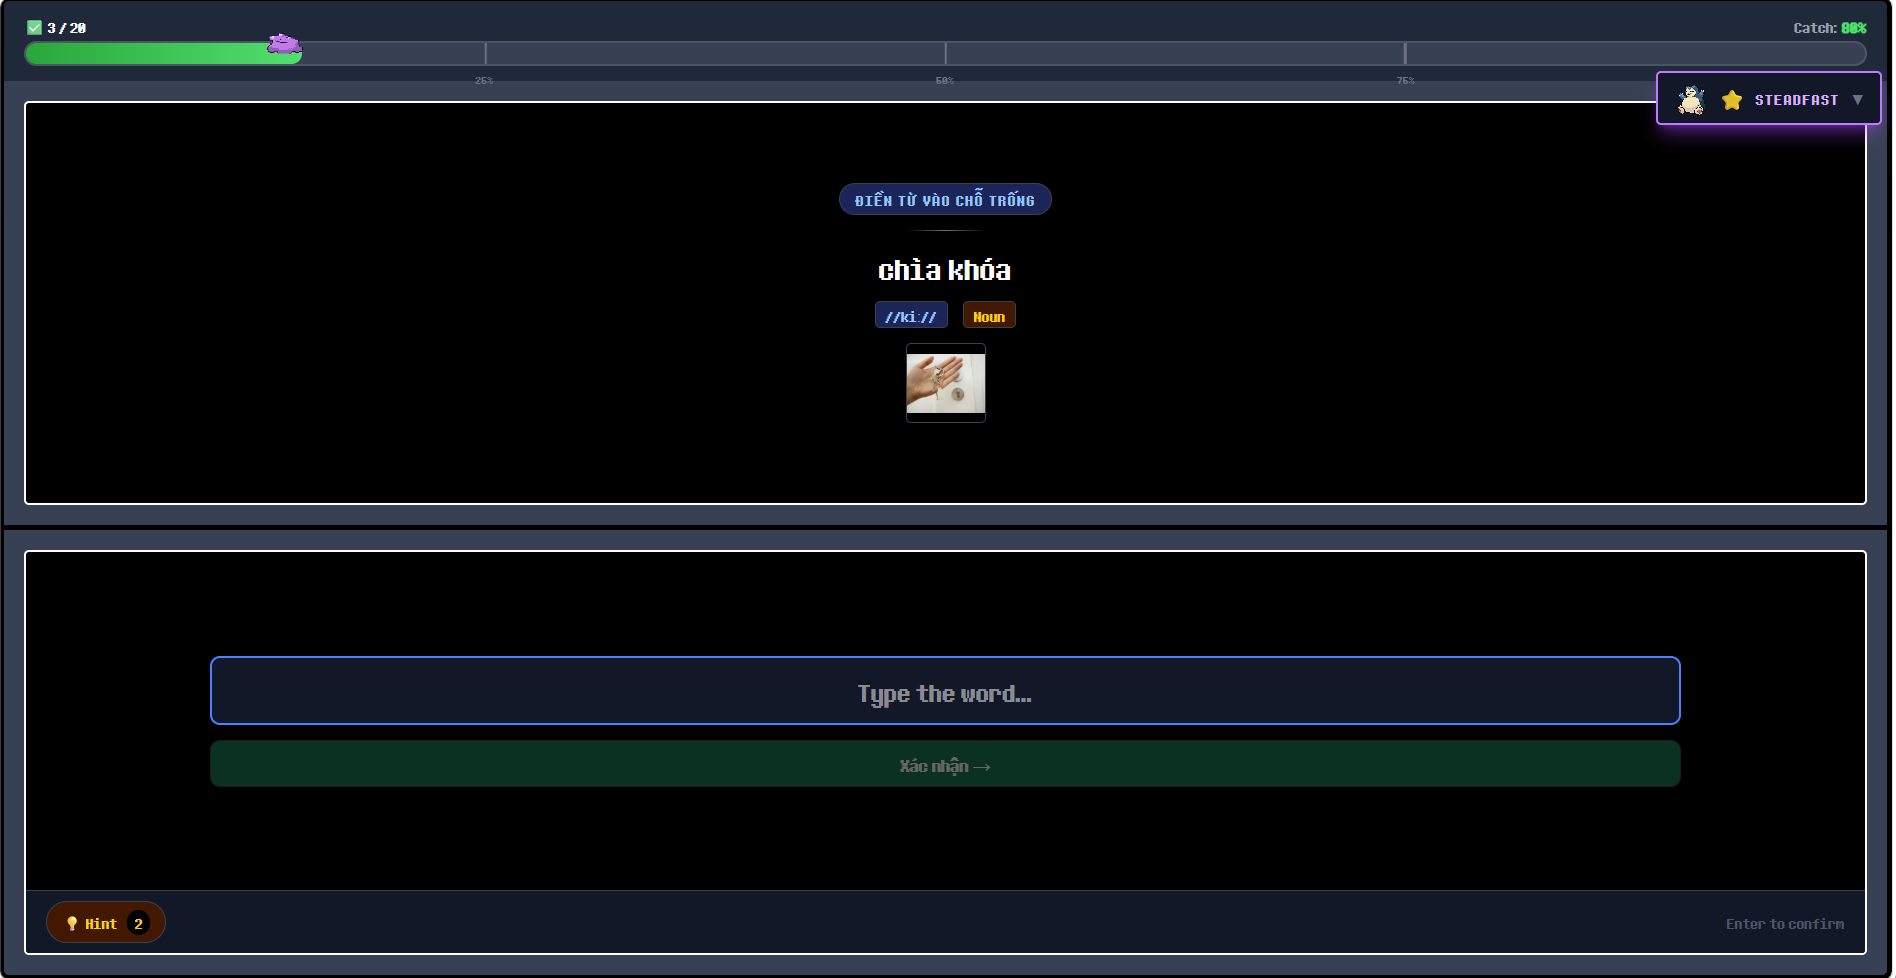
\includegraphics[width=15cm]{images/Final_IF_Session.png}
\caption{Màn hình thực hiện phiên học từ vựng.}
\label{fig:ch3_session}
\end{figure}

\begin{figure}[H]
\centering
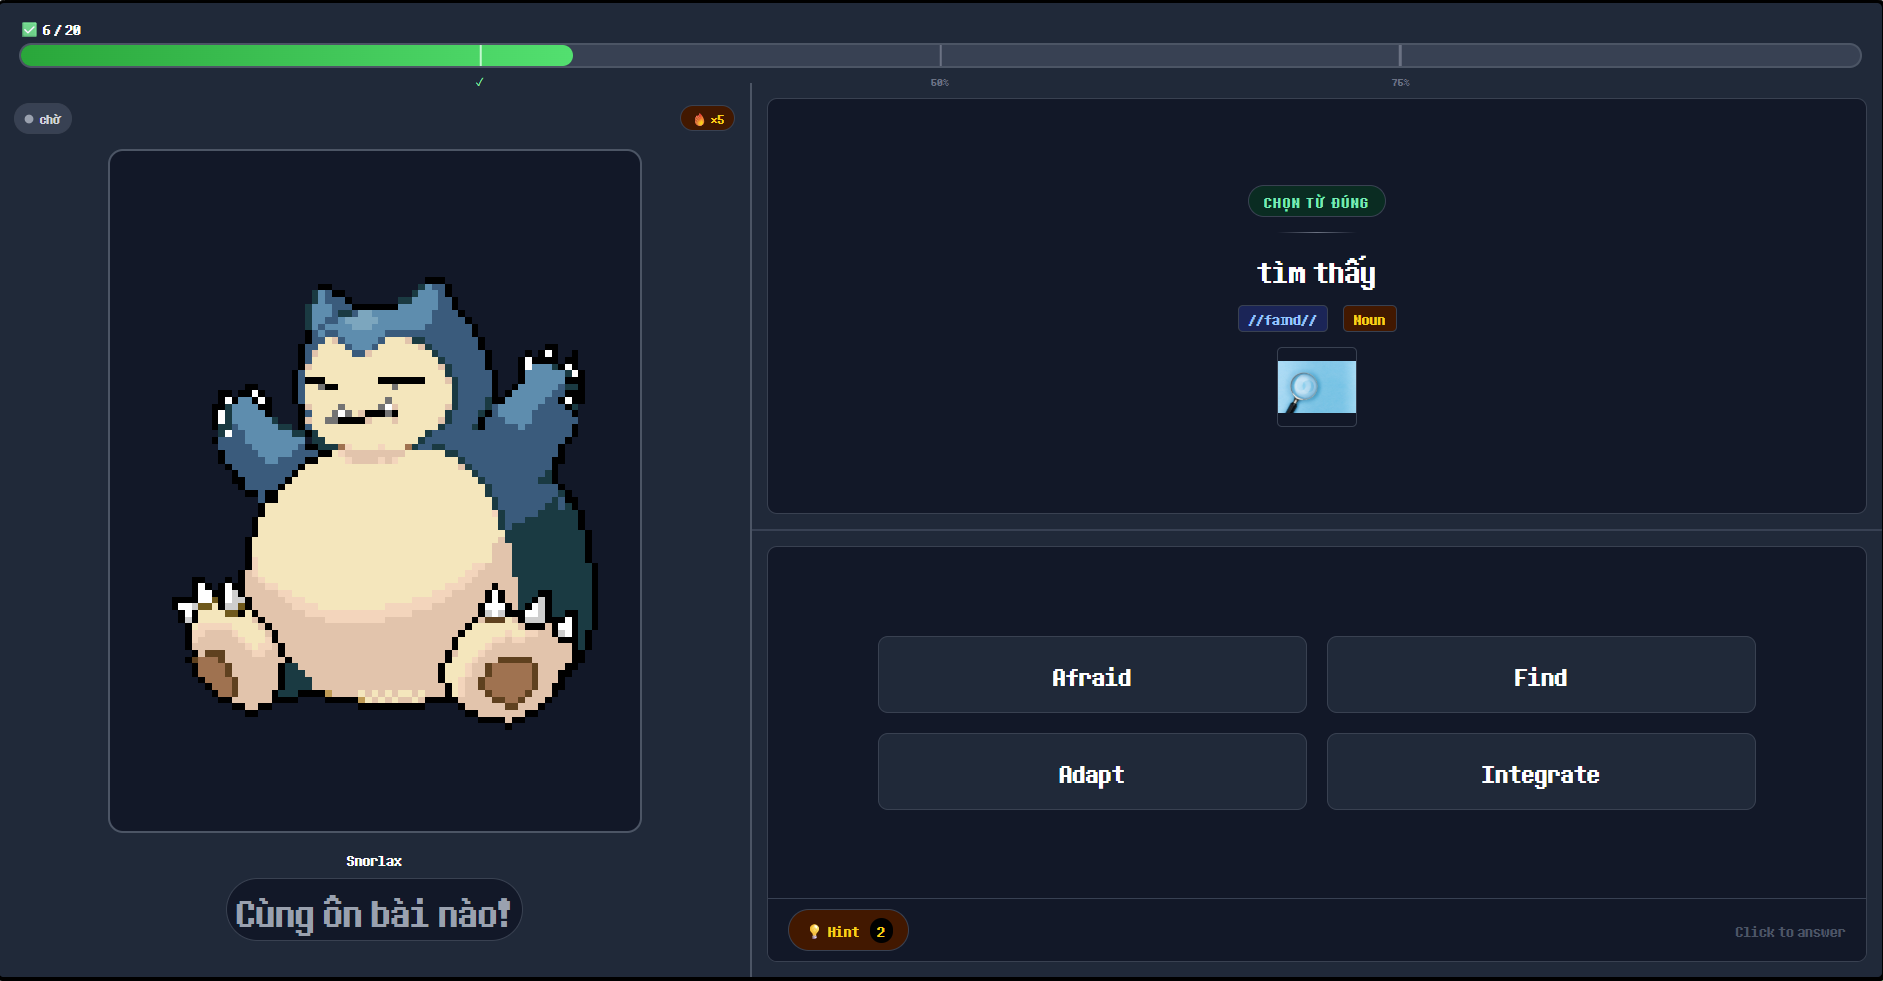
\includegraphics[width=15cm]{images/Final_IF_ReviewSession.png}
\caption{Màn hình thực hiện phiên ôn tập từ vựng.}
\label{fig:ch3_review_session}
\end{figure}


Hệ thống thiết lập một cơ chế phần thưởng phân cấp nhằm tối ưu hóa động lực học tập dựa trên độ khó của nhiệm vụ nhận thức. Cụ thể, các chỉ số phần thưởng được quy định chi tiết trong bảng dưới đây:

\begin{table}[H]
\centering
\caption{Quy tắc quy đổi phần thưởng sau khi hoàn thành phiên tương tác.}
\label{tab:ch3_reward_system}
\renewcommand{\arraystretch}{1.2}
\begin{tabular}{|l|c|c|l|}
\hline
\textbf{Loại phiên tương tác} & \textbf{XP cơ bản} & \textbf{XP cho Thú ảo} & \textbf{Phần thưởng bổ sung} \\ \hline
Phiên học mới (Learning) & 20 XP & +100 XP & Cơ hội bắt Thú ảo mới \\ \hline
Phiên ôn tập (Review) & 100 XP & +100 XP & +3 AP (Điểm thành tích) \\ \hline
\end{tabular}
\end{table}

Điểm đáng chú ý trong thiết kế cân bằng là mức kinh nghiệm cơ bản (base XP) của phiên ôn tập được thiết lập cao gấp năm lần so với phiên học mới. Sự chênh lệch này không phải là ngẫu nhiên mà xuất phát từ nguyên lý tâm lý học hành vi: quá trình ôn tập đòi hỏi sự nỗ lực truy hồi (retrieval effort) lớn hơn để tái hiện kiến thức từ trí nhớ dài hạn so với việc tiếp nhận thông tin mới ở mức độ nhận diện ban đầu. Bằng cách ưu tiên giá trị phần thưởng cho hoạt động ôn tập, hệ thống gián tiếp thúc đẩy người học duy trì sự kỷ luật đối với lộ trình lặp lại ngắt quãng, vốn là yếu tố then chốt để chuyển dịch thông tin thành kiến thức bền vững. 

Bên cạnh XP cho người dùng, mỗi phiên hoàn thành đều đóng góp 100 XP pet để nâng cấp thú ảo đang kích hoạt, tạo ra sự tịnh tiến song song giữa năng lực ngôn ngữ của người học và sự phát triển của sinh vật đồng hành. Đối với các phiên ôn tập, người học còn nhận thêm 3 điểm AP (Achievement Points) dùng cho các giao dịch đặc biệt, trong khi phiên học mới cung cấp cơ hội bắt giữ thú ảo với tỷ lệ thành công (Catch Rate) biến thiên dựa trên hiệu suất trả lời đúng của chính phiên đó.

Hai loại phiên tương tác phục vụ hai mục đích nhận thức khác nhau và do đó áp dụng chiến lược lựa chọn từ vựng khác biệt. Phiên học mới (SessionType.Learning) truy vấn từ vựng chưa từng tiếp cận từ một bộ cụ thể thông qua GetUnlearnedVocabulariesFromSetAsync, giới hạn mặc định 5 từ mỗi phiên; phiên ôn tập (SessionType.Review) hoạt động xuyên bộ từ — ISRSService.GetDueVocabulariesAsync quét toàn bộ tiến trình của người dùng và chọn những từ có NextReviewTime đến hạn, đảm bảo tuân thủ lịch ôn tập tối ưu theo SM-2. Hệ thống còn bảo vệ tính liên tục của tiến trình bằng cơ chế tiếp nối tự động (session resume): trước khi khởi tạo session mới, cả hai luồng đều kiểm tra sự tồn tại của session chưa hoàn thành — nếu có, số câu đã trả lời đúng được khôi phục từ \textbf{AnswerRecord} và session cũ được trả lại thay vì tạo mới, tránh mất tiến trình khi người dùng thoát giữa chừng.

Một điểm kỹ thuật quan trọng trong thiết kế hiệu ứng buff là nguyên tắc "đóng băng tại thời điểm tạo" (snapshot-at-creation): khi session được khởi tạo, PetBuffService.GetActivePetBuffAsync được gọi đúng một lần và toàn bộ giá trị buff (XpMultiplier, CatchRateBonus, HasHintShield, ReducePenalty) được ghi trực tiếp vào bản ghi \textbf{LearningSession}. Tỷ lệ bắt thú ảo cũng được cập nhật ngay lập tức: $CatchRate \mathrel{+}= PetCatchBonus$. Thiết kế này đảm bảo tính nhất quán của phiên học — người dùng không thể thay đổi thú ảo đang kích hoạt để tăng lợi thế sau khi session đã bắt đầu.

Trong mỗi câu hỏi, cơ chế tiến hoặc lùi cấp độ (level progression) vận hành theo nguyên tắc hai chiều: trả lời đúng tăng CurrentLevel lên 1, đạt level 4 thì từ được đánh dấu hoàn thành; trả lời sai thì CurrentLevel giảm 1 (tối thiểu về 0) — từ quay về dạng câu hỏi dễ hơn. Thuật toán SM-2 chỉ được kích hoạt khi một từ hoàn thành tất cả 4 cấp trong phiên ôn tập. Lúc này, điểm chất lượng (grade 0–5) được tính bởi hàm CalculateSm2Grade dựa trên bốn yếu tố: tính chính xác (isCorrect), số lần sai tích lũy (attemptCount), thời gian phản hồi trung bình (avgResponseTime) và số gợi ý đã sử dụng (totalHints). Cụ thể: grade 5 (hoàn hảo) khi không sai, trả lời trong 5 giây và không dùng gợi ý; grade 4 khi không sai nhưng mất hơn 5 giây; grade 3 khi sai tối đa 1 lần; grade 2 khi sai 2 lần — phản ánh đúng mức độ nỗ lực truy hồi thực tế. Ngưỡng 5 giây là một ngưỡng thực nghiệm (heuristic threshold) dựa trên quan sát rằng thời gian phản hồi ngắn (dưới 3--5 giây) thường được đồng nhất với quá trình truy hồi tự động (automatic retrieval), trong khi phản hồi chậm hơn chỉ ra từ vựng vẫn cần nỗ lực có ý thức \cite{Carpenter2012}. Ngưỡng này cần được hiệu chỉnh thêm qua dữ liệu người dùng thực tế trong các giai đoạn thực nghiệm tiếp theo. Toàn bộ kết quả SM-2 (EaseFactor trước/sau, Interval trước/sau, NextReviewDate) được lưu vào \textbf{VocabularyReviewHistory}, tạo nhật ký đầy đủ theo từng lượt ôn.

Khi hoàn thành session, hệ thống kích hoạt một chuỗi nghiệp vụ tuần tự: XP cơ bản được nhân với PetXpMultiplier được lưu trong session; nếu thú ảo phần thưởng đã thuộc sở hữu của người học, GrantPetAsync trả về bonusXp bổ sung thay thế; thú ảo đang kích hoạt nhận 100 XP cố định (áp dụng cho cả Learning lẫn Review), có thể dẫn tới level-up hoặc tiến hóa; nhiệm vụ hàng ngày được cập nhật tương ứng (QuestType.Learn hoặc QuestType.Review); cuối cùng, GymLeaderService.CheckAndUnlockGymsAsync được gọi theo kiểu fire-and-forget để kiểm tra điều kiện mở khóa Gym mới — lỗi trong bước này không làm gián đoạn phản hồi trả về cho người học.

Giao diện phiên học phân biệt hai chế độ bố cục: chế độ learning sử dụng màn hình chia đôi theo chiều dọc — nửa trên hiển thị thú ảo và hình ảnh ngữ cảnh (GameScreen), nửa dưới chứa câu hỏi và khu vực nhập đáp án (AnswerScreen); chế độ review sử dụng ReviewLayout với thú ảo đang kích hoạt của người dùng làm nhân vật đồng hành. Trước khi phiên học mới bắt đầu, hệ thống hiển thị màn hình gặp gỡ (PokemonEncounterIntro) giới thiệu thú ảo sẽ xuất hiện, tạo cảm giác kỳ vọng theo cơ chế tường thuật. Trong suốt phiên, ba ngưỡng cột mốc được theo dõi tại 5, 10 và 15 câu trả lời đúng, tương ứng với các mức hoàn thành 25\%, 50\% và 75\% — mỗi ngưỡng kích hoạt một lớp phủ động lực (MilestoneOverlay) hiển thị thông điệp khích lệ và xác nhận tiến trình, ứng dụng nguyên lý phản hồi tức thì để duy trì trạng thái tập trung (flow state) của người học.

\subsection{Cơ chế kiến tạo và quản trị học liệu cá nhân}

Phân hệ kiến tạo bộ từ vựng được thiết kế theo luồng bốn bước, kết hợp giữa tự động hóa AI và kiểm soát chủ động của người học.

\textbf{Bước 1} yêu cầu người dùng xác lập siêu dữ liệu (metadata) của bộ học liệu: tiêu đề (tối đa 100 ký tự), mô tả (tối đa 300 ký tự), chủ đề (VocabularySetTheme), mức độ thử thách (DifficultyLevel), chế độ riêng tư hay công khai và ảnh đại diện (tối đa 5 MB). Toàn bộ đầu vào được kiểm tra phía Frontend trước khi gửi lên Backend, bao gồm lọc bỏ ký tự HTML < và > nhằm phòng ngừa tấn công injection. \textbf{Bước 2} tiếp nhận danh sách từ vựng qua hai phương thức: nhập tay (phân cách bởi xuống dòng hoặc dấu phẩy, tối đa 50 từ) hoặc nhập hàng loạt bằng cách tải lên tệp định dạng .csv hay .txt — giải phóng người học khỏi thao tác gõ tay lặp lại. Người dùng có thể bật hoặc tắt chế độ AI để lựa chọn giữa sinh metadata tự động và nhập thủ công.

\textbf{Bước 3} là giai đoạn then chốt của quy trình: Backend gọi AiPreviewVocabularySetAsync và trả về danh sách kết quả dự thảo. Mỗi phần tử mang một trong ba cờ trạng thái — isAiGenerated (AI sinh ra), isExisting (từ đã có sẵn trong hệ thống) hoặc isCustom (người dùng thêm thủ công) — giúp phân biệt rõ nguồn gốc dữ liệu. Thay vì tiếp nhận kết quả AI một cách thụ động, giao diện trao toàn quyền chỉnh sửa: người dùng có thể hiệu chỉnh từng trường (nghĩa, phiên âm, câu ví dụ, mô tả) trực tiếp trên bảng, thêm hàng mới, xóa hàng không cần thiết và chọn hay bỏ chọn từng từ trước khi xác nhận tạo. Vòng lặp "human-in-the-loop" này đảm bảo chất lượng học liệu luôn được kiểm soát bởi người học, không phụ thuộc hoàn toàn vào đầu ra của mô hình ngôn ngữ. \textbf{Bước 4} hiển thị kết quả tạo thành công và điều hướng về bộ từ vừa khởi tạo.

Một quyết định thiết kế quan trọng ẩn sau bước 3 là cơ chế tách biệt ngữ cảnh dữ liệu (SetVocabulary Override). Khi một từ trả về với isExisting = true và người dùng chỉnh sửa các trường thông tin, thay đổi không được ghi vào bản ghi \textbf{Vocabularies} gốc — bảng dữ liệu trung tâm dùng chung toàn hệ thống. Thay vào đó, chỉ bảng liên kết \textbf{SetVocabulary} của bộ đó được cập nhật. Cơ chế này cho phép mỗi người dùng tùy biến ngữ cảnh riêng (ví dụ, câu ví dụ theo chuyên ngành) cho cùng một từ mà không làm ảnh hưởng đến dữ liệu nền tảng chung, đồng thời tránh tạo bản ghi trùng lặp không cần thiết trong cơ sở dữ liệu.

Tính gắn kết chủ đề giữa nội dung học tập và hệ thống Gamification được hiện thực hóa qua ThemeToPetTypesMap — một ánh xạ tĩnh liên kết từng VocabularySetTheme với một hoặc nhiều PetType tương ứng: Nature → Grass, Technology → Electric, Food → Fire, Science → Psychic, Mystery → Ghost. Khi tạo bộ từ, hệ thống dựa vào ánh xạ này để lựa chọn \textbf{SetRewardPet} ưu tiên — danh sách thú ảo có thể xuất hiện sau mỗi phiên học thành công — đảm bảo tính tường thuật nhất quán giữa chủ đề nội dung và phần thưởng nhận được.

Trang khám phá bộ từ vựng phản ánh thêm một quyết định kỹ thuật đáng ghi nhận về hiệu năng: thay vì gửi N yêu cầu riêng lẻ theo từng chủ đề, Frontend sử dụng endpoint GetGroupedVocabularySetsAsync để nhận toàn bộ dữ liệu đã gom nhóm theo Theme trong một lần truy vấn duy nhất. Giải pháp này loại bỏ lỗi N+1 Query, đồng thời giảm số vòng gọi API tỷ lệ thuận với số chủ đề đang hoạt động. Bên cạnh chế độ danh sách thông thường, trang còn cung cấp chế độ bản đồ (Map View) trực quan hóa các chủ đề theo vùng không gian địa lý ảo, nơi người dùng nhấp vào từng điểm nóng (hotspot) để khám phá bộ từ theo chủ đề tương ứng, nâng cao trải nghiệm khám phá nội dung.

\begin{figure}[H]
\centering
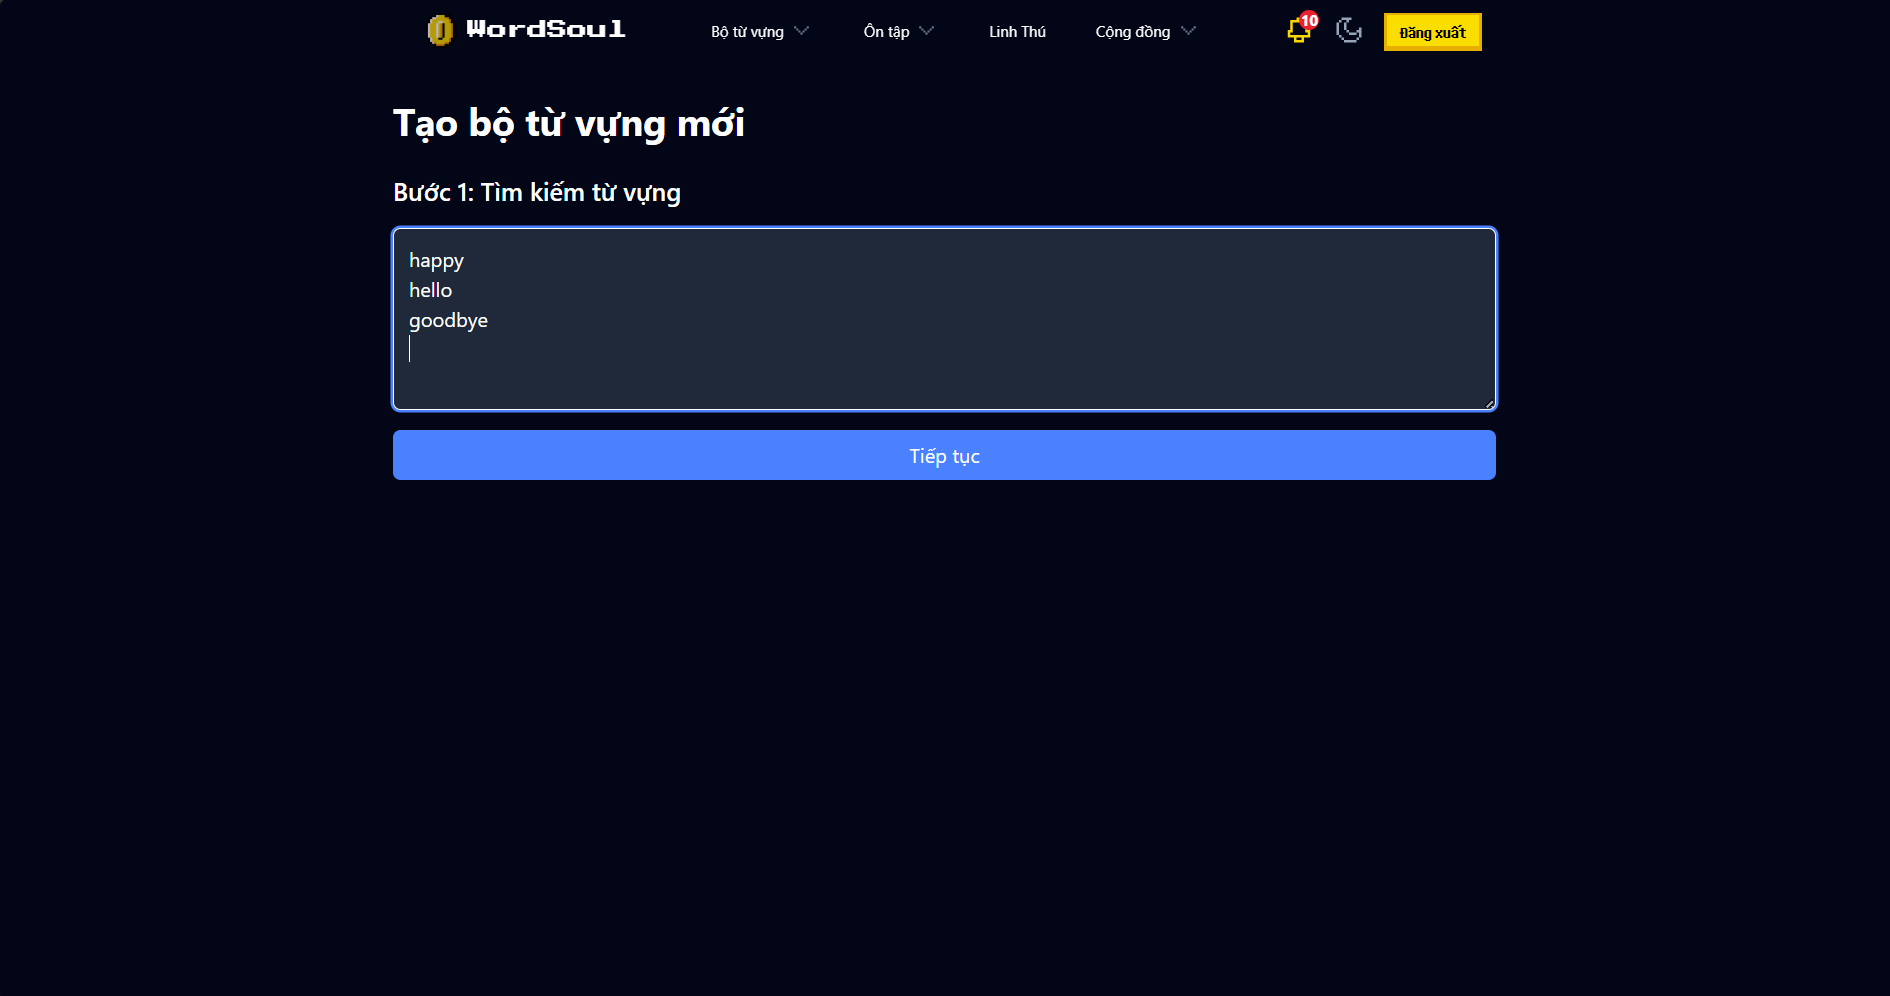
\includegraphics[width=15cm]{images/Final_IF_Set1.png}
\caption{Giao diện khởi tạo thuộc tính bộ từ vựng.}
\label{fig_set1}
\end{figure}

\begin{figure}[H]
\centering
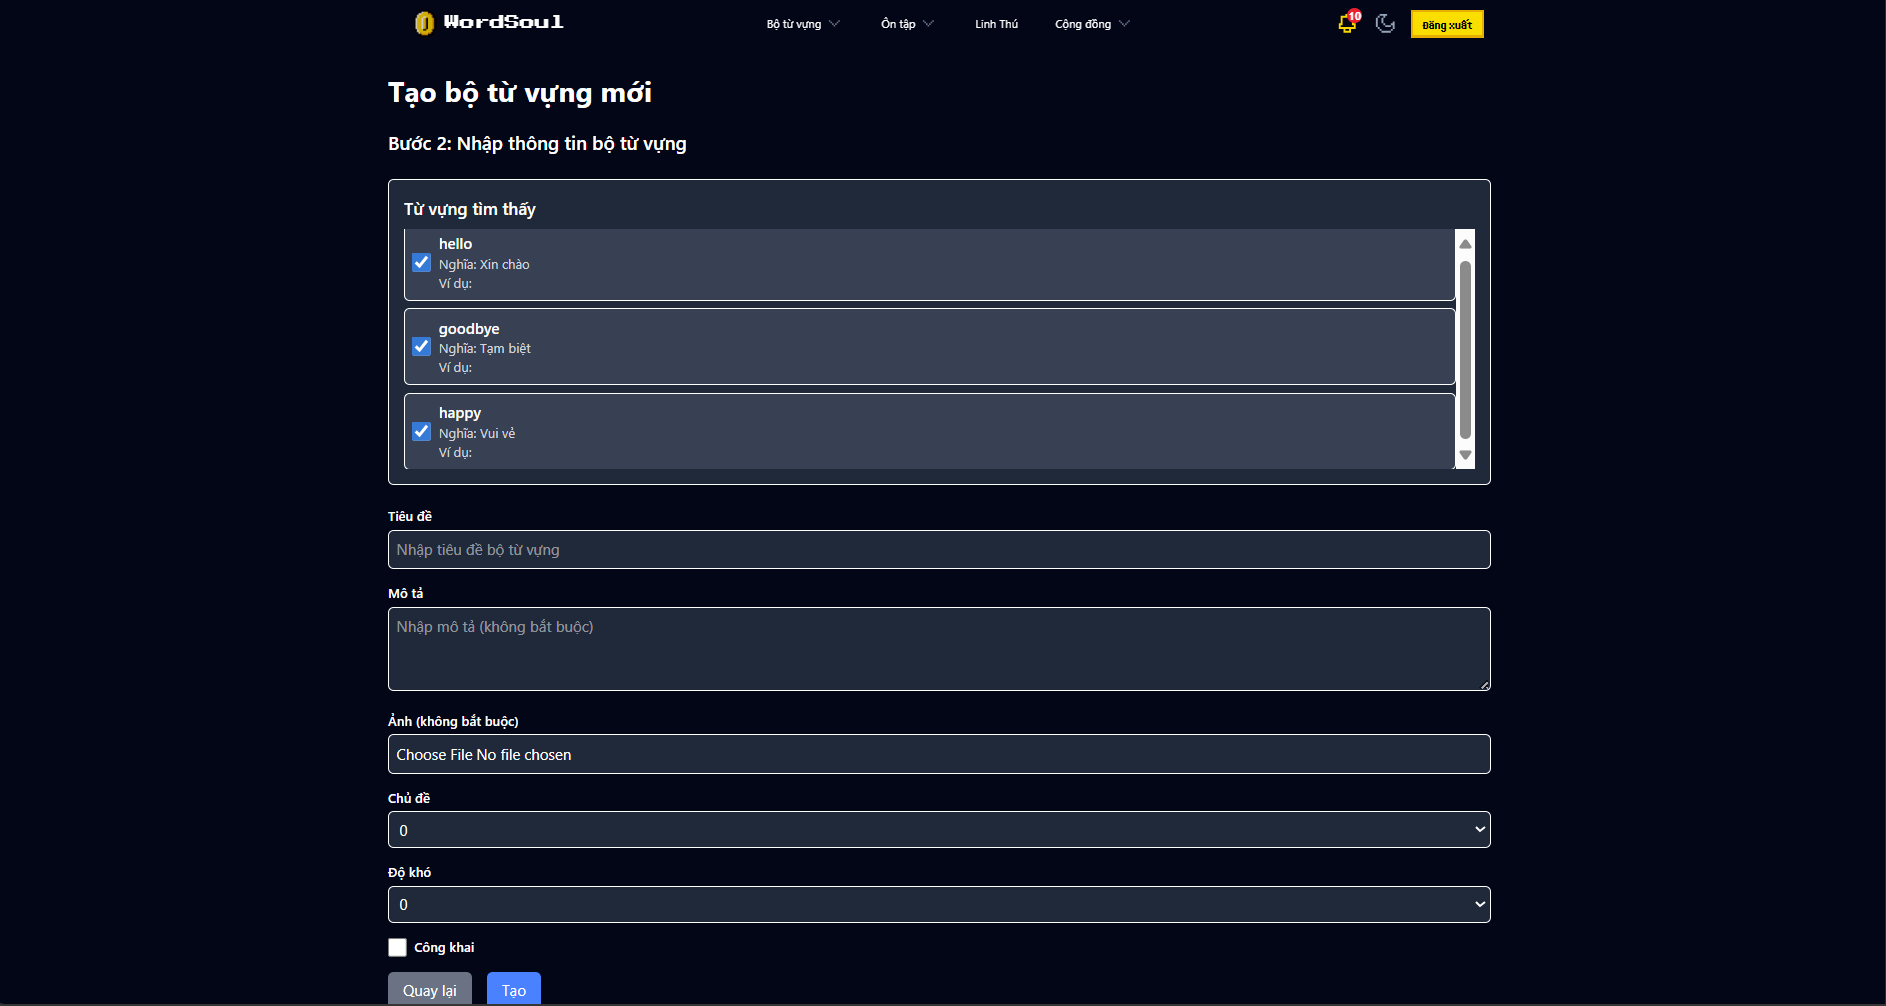
\includegraphics[width=15cm]{images/Final_IF_Set2.png}
\caption{Quy trình tuyển chọn đơn vị kiến thức cho bộ từ.}
\label{fig_set2}
\end{figure}

\subsection{Hệ thống sinh vật ảo và logic tiến hóa}

Hệ thống thú ảo được triển khai như một trụ cột chiến lược trong mô hình Gamification, có nhiệm vụ chuyển hóa các nỗ lực học thuật thành những thực thể số có khả năng tương tác sinh động. Mỗi sinh vật trong hệ thống được định danh bởi một tập hợp các chỉ số đặc trưng, từ cấp độ hiếm (Rarity), thuộc tính nguyên tố cho đến chu kỳ sinh trưởng.

Mối liên kết hữu cơ giữa hiệu suất học tập và giá trị giải trí được thể hiện rõ nhất qua thuật toán bắt giữ thú ảo (Catch Mechanism). Chỉ số thành công (Catch Rate) không còn là một biến số ngẫu nhiên đơn thuần mà bị chi phối trực tiếp bởi chất lượng phản hồi của người học. Hệ thống áp dụng một cơ chế phạt logic: với mỗi sai sót trong phiên học, khả năng sở hữu thú ảo sẽ bị khấu trừ 5\% ($-0.05$). Quy tắc này đặt người dùng vào trạng thái tập trung tối đa, nơi năng lực học thuật trở thành chìa khóa duy nhất để chinh phục những thực thể quý hiếm (Bảng \ref{tab:catch_rate}).

\begin{table}[H]
\centering
\caption{Bảng tham chiếu tỷ lệ thu phục dựa trên phân cấp độ hiếm.}
\label{tab:catch_rate}
\renewcommand{\arraystretch}{1.2}
\begin{tabular}{|l|c|l|}
\hline
\textbf{Phân loại (Rarity)} & \textbf{Xác suất cơ bản} & \textbf{Đặc điểm vận hành} \\ \hline
Common & 1.0 (100\%) & Luôn đạt được khi hoàn thành phiên học. \\ \hline
Uncommon & 0.8 (80\%) & Yêu cầu sự cẩn trọng để bảo toàn tỷ lệ. \\ \hline
Rare & 0.6 (60\%) & Dễ thất bại nếu tần suất sai sót cao. \\ \hline
Epic & 0.4 (40\%) & Thử thách lớn đối với khả năng truy hồi kiến thức. \\ \hline
Legendary & 0.2 (20\%) & Chỉ dành cho những phiên học đạt độ chính xác tuyệt đối. \\ \hline
\end{tabular}
\end{table}

Bên cạnh việc thu thập, lộ trình phát triển của thú ảo (Level Up \& Evolution) đóng vai trò duy trì sự gắn kết dài hạn thông qua việc tích lũy kinh nghiệm (XP). Logic tiến hóa được thiết kế như một quá trình chuyển đổi trạng thái (State Transition) chặt chẽ: khi các điều kiện về RequiredLevel và NextEvolutionId được thỏa mãn, hệ thống sẽ thực thi lệnh thay đổi định danh PetId sang hình thái mới. 

Quy trình này không chỉ là sự thay đổi về mặt đồ họa mà còn là sự công nhận cho nỗ lực trí tuệ của người học. Việc sở hữu những thú ảo ở hình thái cấp cao chính là sự hiện thực hóa nhu cầu khẳng định năng lực (Competence) theo Thuyết Tự Quyết, tạo ra niềm tự hào và động lực nội tại mạnh mẽ \cite{WerbachHunter2012}.

\begin{figure}[H]
\centering
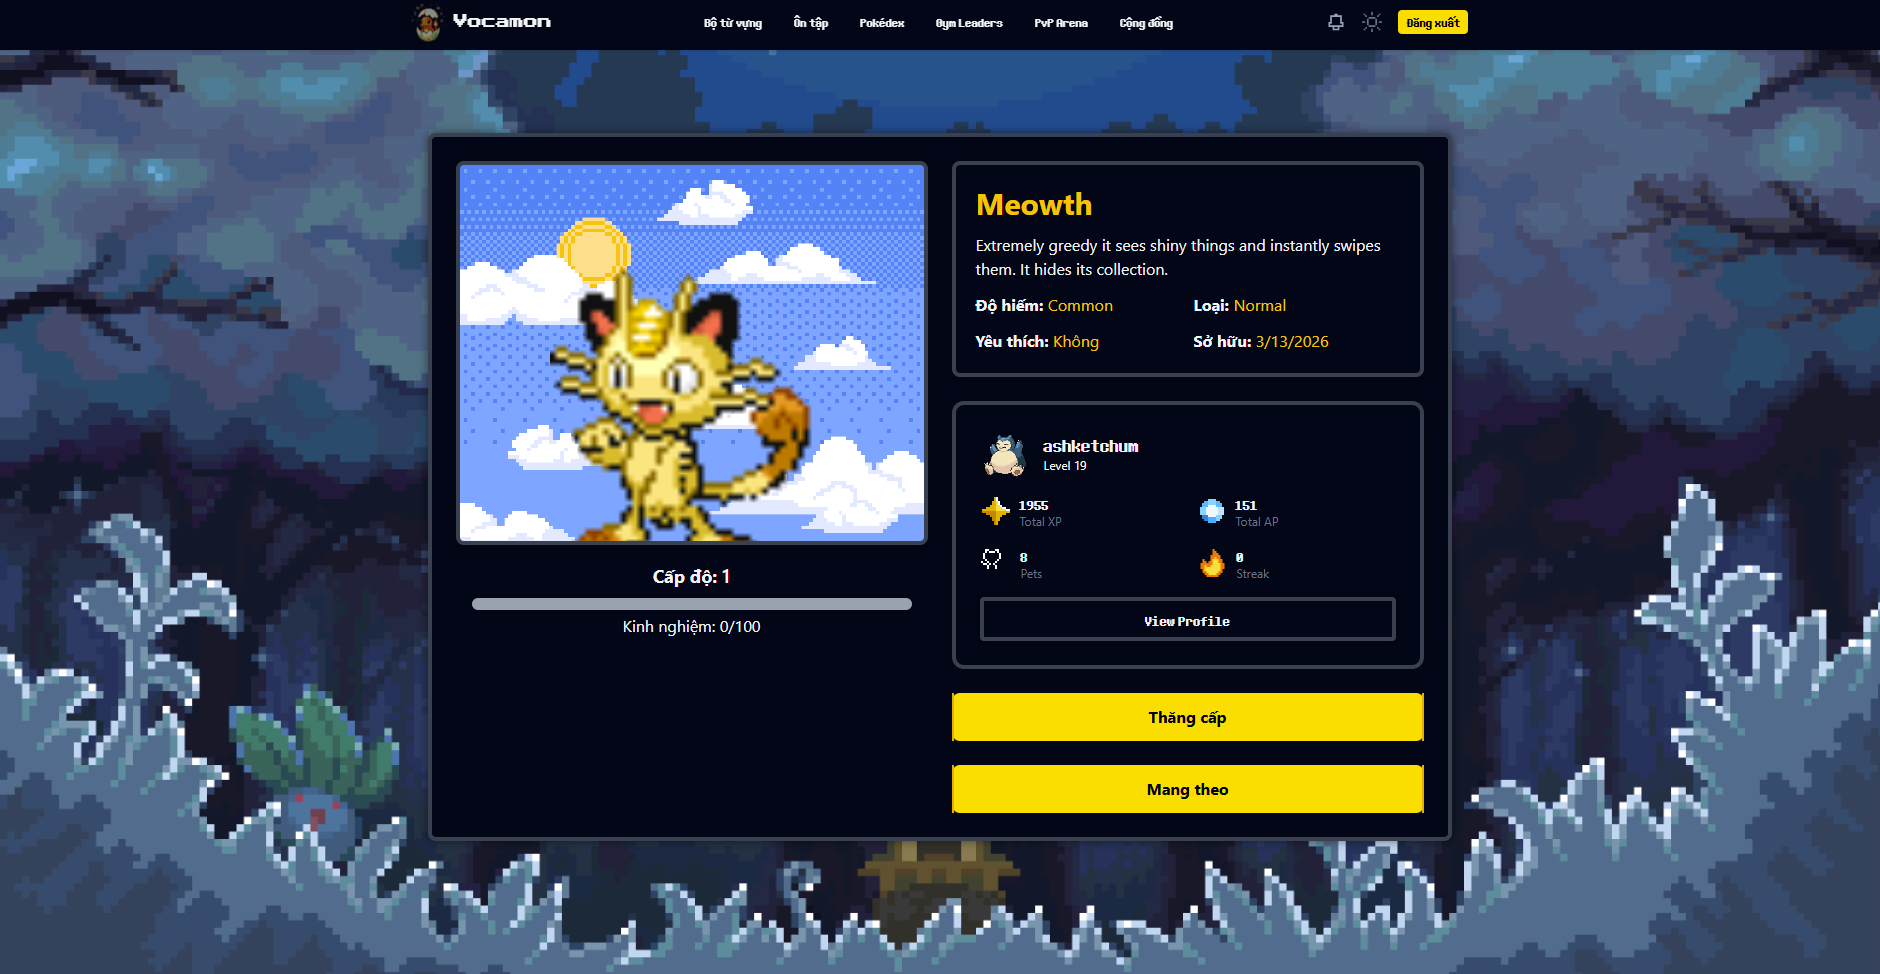
\includegraphics[width=15cm]{images/Final_IF_Pet.png}
\caption{Giao diện quản lý và nâng cấp thực thể ảo.}
\label{fig_pet}
\end{figure}

\subsection{Bảng điều khiển trung tâm và Quản trị hiệu suất}

Dashboard được thiết kế để đảm nhận vai trò là bộ não điều phối và phân tích kết quả học tập của người dùng. Vượt xa khỏi khái niệm một trang đích tĩnh, giao diện này vận hành như một trung tâm dữ liệu thông minh, nơi các thông tin thô từ lịch sử học tập được mô hình hóa thành các biểu đồ trực quan về mức độ thành thạo ngôn ngữ. Thông qua việc theo dõi các chỉ số tịnh tiến như điểm kinh nghiệm (XP), cấp độ và chuỗi rèn luyện (streak), người học có thể tự đánh giá một cách khách quan về cường độ và chất lượng của lộ trình cá nhân.

Sự giao thoa giữa các chỉ số định lượng và hệ thống mục tiêu định kỳ tạo ra một áp lực tích cực lên tâm lý người học. Việc tích hợp các nhiệm vụ ngắn hạn song song với các thành tựu dài hạn ngay tại màn hình chính giúp người dùng luôn định vị được vị trí của mình trong bức tranh tổng thể. Dưới góc độ tâm lý học hành vi, phương thức này đã khai thác triệt để nhu cầu về sự tự chủ và tính chuyên môn, chuyển đổi tâm thế từ việc học theo nghĩa vụ sang việc chủ động duy trì kỷ luật. Đây chính là "điểm chạm" quan trọng giúp tối ưu hóa khả năng hoàn thành các mục tiêu tri thức và xây dựng một thói quen học tập bền vững \cite{RyanDeci2017}.

\begin{figure}[H]
\centering
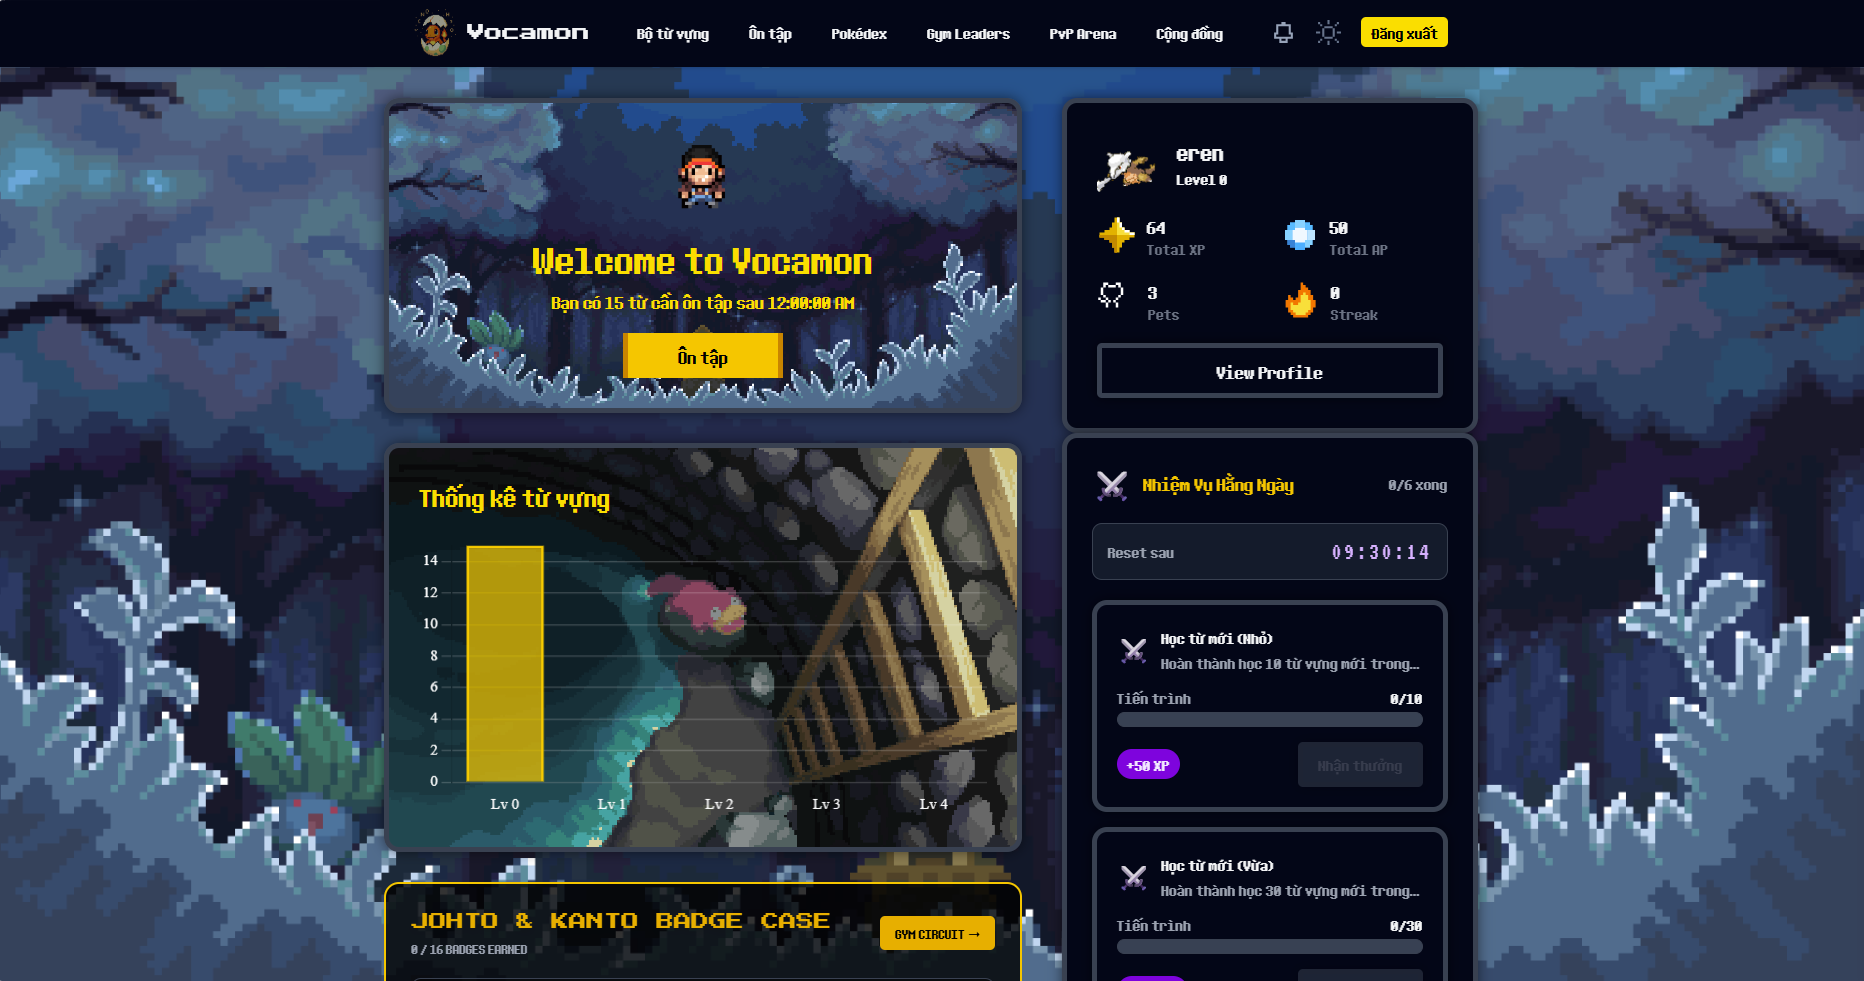
\includegraphics[width=15cm]{images/Final_IF_Static.png}
\caption{Tổng quan giao diện phân tích tiến độ người dùng.}
\label{fig_dashboard}
\end{figure}


\subsection{Hệ thống đối kháng PvP và PvE}


Phân hệ đối kháng đã được triển khai thành công, không chỉ làm phong phú thêm các hình thức tương tác mà còn tạo ra chiều sâu chiến thuật cho hệ thống học tập. Chế độ đối kháng giữa người với người (PvP) vận hành dựa trên cơ chế ghép trận tự động (Matchmaking) thông qua chỉ số Elo, giúp đảm bảo tính cân bằng và duy trì môi trường cạnh tranh lành mạnh giữa những người học có cùng trình độ năng lực. Bên cạnh khả năng ghép trận ngẫu nhiên, hệ thống còn hỗ trợ tính năng tạo phòng riêng biệt và kết nối thông qua mã mời, đáp ứng nhu cầu học tập tương tác trong các nhóm nhỏ hoặc cộng đồng cụ thể. Sự linh hoạt này giúp chuyển hóa việc học từ vựng từ một hoạt động cá nhân đơn thuần thành một trải nghiệm kết nối xã hội đầy hứng thú.

Song song với đó, chế độ thách đấu với hệ thống (PvE) hiện thực hóa một lộ trình tiến bộ có thứ bậc nghiêm ngặt thông qua mô hình tám Gym Leader được sắp xếp tăng dần về độ khó (GymOrder từ 1 đến 8). Điều kiện mở khóa mỗi Gym Leader được định nghĩa bằng hai ngưỡng kép trong thực thể GymLeader: XpThreshold — tổng điểm kinh nghiệm tích lũy của người dùng — và VocabThreshold — số lượng từ vựng đã đạt tối thiểu trạng thái học tập yêu cầu với cấp độ CEFR không thấp hơn RequiredCefrLevel. Cơ chế này đảm bảo người học chỉ được tiếp cận thử thách nâng cao khi đã thực sự tích lũy đủ vốn từ theo chuẩn quốc tế, chứ không đơn thuần dựa vào thời gian tham gia.

Trạng thái tiến trình của mỗi cặp (người dùng, Gym Leader) được theo dõi thông qua thực thể UserGymProgress với ba trạng thái: Locked (chưa đủ điều kiện), Unlocked (đã mở khóa, chưa chinh phục) và Defeated (đã chinh phục). Sau mỗi lần thất bại, hệ thống kích hoạt cơ chế cooldown tính từ LastAttemptAt, ngăn cản chiến lược brute-force và khuyến khích người học ôn tập từ vựng giữa các lần thử. Điểm số cao nhất từng đạt được (BestScore) được lưu trữ độc lập nhằm cung cấp phản hồi khách quan về sự cải thiện dần dần. Khi lần đầu tiên chinh phục thành công một Gym Leader, hệ thống tự động cấp BadgeAchievement — một thành tích đặc biệt gắn liền với huy hiệu (Badge) của Gym đó — khép kín vòng lặp phần thưởng dài hạn giữa hệ thống PvE và hệ thống thành tích. Điểm cốt lõi trong tính năng này là việc ứng dụng giao thức SignalR để xử lý toàn bộ logic chiến đấu dưới dạng thời gian thực, trong đó sự kết hợp giữa tốc độ phản xạ và độ chính xác của từ vựng trở thành yếu tố quyết định thắng bại.

Hệ thống PvP cung cấp ba luồng vào trận biệt lập. Luồng thứ nhất — Room Code: người chơi A tạo phòng qua POST /api/pvp/create, nhận cặp \{sessionId, roomCode\}, chia sẻ mã mời cho đối thủ; người chơi B gửi POST /api/pvp/join kèm roomCode để gia nhập. Luồng thứ hai — Matchmaking tự động: cả hai phía gọi POST /api/pvp/queue/join kèm ConnectionId của SignalR Hub đang kết nối. MatchmakingQueueService sử dụng ConcurrentDictionary<string, MatchmakingEntry> đảm bảo an toàn luồng (thread-safe), lưu trữ thông tin ELO, thời điểm gia nhập hàng đợi và danh sách thú ảo đã chọn. Thuật toán ghép cặp vận hành theo cơ chế cửa sổ ELO mở rộng: ngưỡng chấp nhận bắt đầu tại ±200 điểm và tăng thêm 50 điểm sau mỗi 10 giây chờ, đảm bảo người chơi chờ lâu vẫn được ghép trận thay vì bị treo vô thời hạn. MatchmakingWorker thực thi vòng quét mỗi 5 giây, tự động gọi CreatePvpSessionAsync cho P1 (Challenger) và JoinPvpSessionAsync cho P2 (Opponent), sau đó thông báo cho cả hai qua IMatchmakingNotifier.NotifyMatchFound mang theo sessionId. Ở cả ba luồng, người chơi phải chọn đúng 3 thú ảo từ bộ sưu tập cá nhân trước khi bắt đầu; nếu sở hữu ít hơn 3 thú ảo, cảnh báo được hiển thị và nút khởi động bị vô hiệu hóa.

Sau khi ghép cặp thành công, cả hai Client kết nối vào BattleHub và gửi tín hiệu PlayerReady. Khi cả hai tín hiệu được tiếp nhận, StartBattleAsync khởi tạo trạng thái đầu trận và đẩy câu hỏi đầu tiên xuống Client qua SignalR. Trong suốt trận đấu, Frontend theo dõi thời điểm bắt đầu mỗi câu hỏi bằng Date.now() và gửi thời gian phản hồi thực tế kèm đáp án; nếu hết giờ, hàm handleTimeup tự động gửi đáp án rỗng. Kết quả mỗi lượt (lastRoundResult) kích hoạt animation tấn công trên sprite: bên gây sát thương chuyển sang trạng thái 'attack', bên bị trúng chuyển sang 'hurt' trong 400 ms, sau đó RoundResultOverlay hiển thị tóm tắt lượt vừa kết thúc. Trận đấu kết thúc khi thỏa một trong ba điều kiện: toàn bộ thú ảo P1 ngã xuống (allP1Fainted), toàn bộ thú ảo P2 ngã xuống (allP2Fainted), hoặc danh sách câu hỏi đã cạn (noMoreQuestions).

Trong chế độ PvE, đối thủ Gym Leader không do người thật điều khiển mà được giả lập bởi ArenaBattleService thông qua tham số BotAccuracy (xác suất trả lời đúng) và BotAvgResponseMs (thời gian phản hồi trung bình). Mỗi lượt, hệ thống tự động quyết định đáp án của bot và gửi kết quả đồng thời với phản hồi của người chơi, tạo ra cảm giác đối kháng thực sự mà không cần đối thủ người thật. Kết thúc trận PvE chiến thắng, màn hình kết quả (BattleArenaResult) hiển thị điểm số đôi bên, độ chính xác, XP nhận được và — nếu là lần chinh phục Gym đầu tiên — huy hiệu thành tích kèm hình ảnh (badgeEarned, badgeName, badgeImageUrl).

Hệ thống PvP duy trì thứ bậc xếp hạng năm tầng dựa trên điểm ELO: Bronze, Silver, Gold, Platinum và Diamond, mỗi tầng được biểu thị bằng màu sắc đặc trưng trên giao diện sảnh chờ (PvpLobby). Sau mỗi trận PvP, điểm ELO được tính lại theo công thức ELO chuẩn — người thắng nhận điểm từ người thua theo tỷ lệ nghịch với chênh lệch hạng — và kết quả thay đổi (eloResult.ratingChange, dương hoặc âm) được hiển thị nổi bật trên màn hình tổng kết (PvpBattleResult) cùng với tầng hiện tại.

Việc tích hợp cơ chế khắc chế thuộc tính (Type Advantage) giữa 18 hệ nguyên tố thú ảo — được tính toán bởi TypeEffectivenessCalculator với ba mức hiệu ứng: Hiệu quả gấp đôi (×2.0), Không mấy hiệu quả (×0.5) và Miễn nhiễm hoàn toàn (×0.0) — cùng với áp lực thời gian trong trận đấu đã hiện thực hóa thành công khái niệm "thử thách có chủ đích" (Desirable Difficulties). Cách tiếp cận này không chỉ giúp củng cố kiến thức một cách bền vững mà còn giúp người học rèn luyện khả năng sử dụng ngôn ngữ linh hoạt trong các tình huống thực tế đòi hỏi phản ứng nhanh. Kết quả đạt được khẳng định tính hiệu quả của việc kết hợp giữa công nghệ truyền tải dữ liệu hiện đại và các nguyên lý trò chơi hóa vào giáo dục ngôn ngữ \cite{Bjork2011, Deterding2011}.

\begin{figure}[H]
\centering
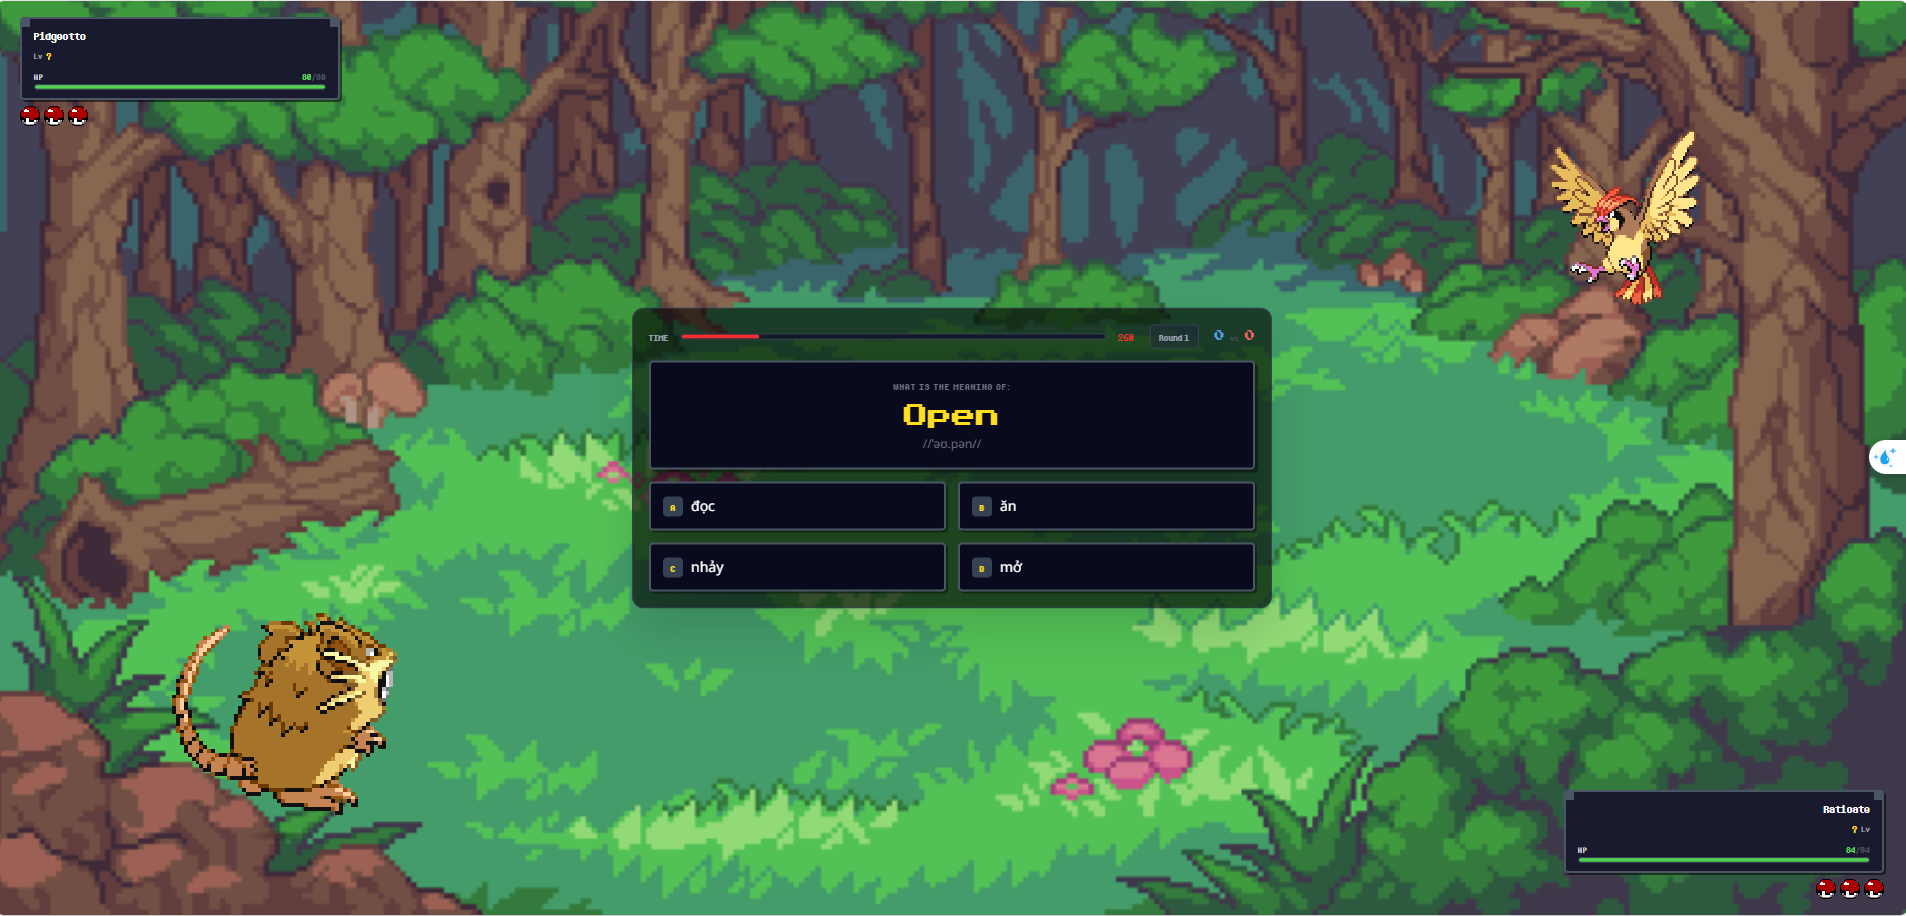
\includegraphics[width=15cm]{images/Final_IF_Battle.png}
\caption{Màn hình chiến đấu đối kháng.}
\label{fig_battle}
\end{figure}

\begin{figure}[H]
\centering
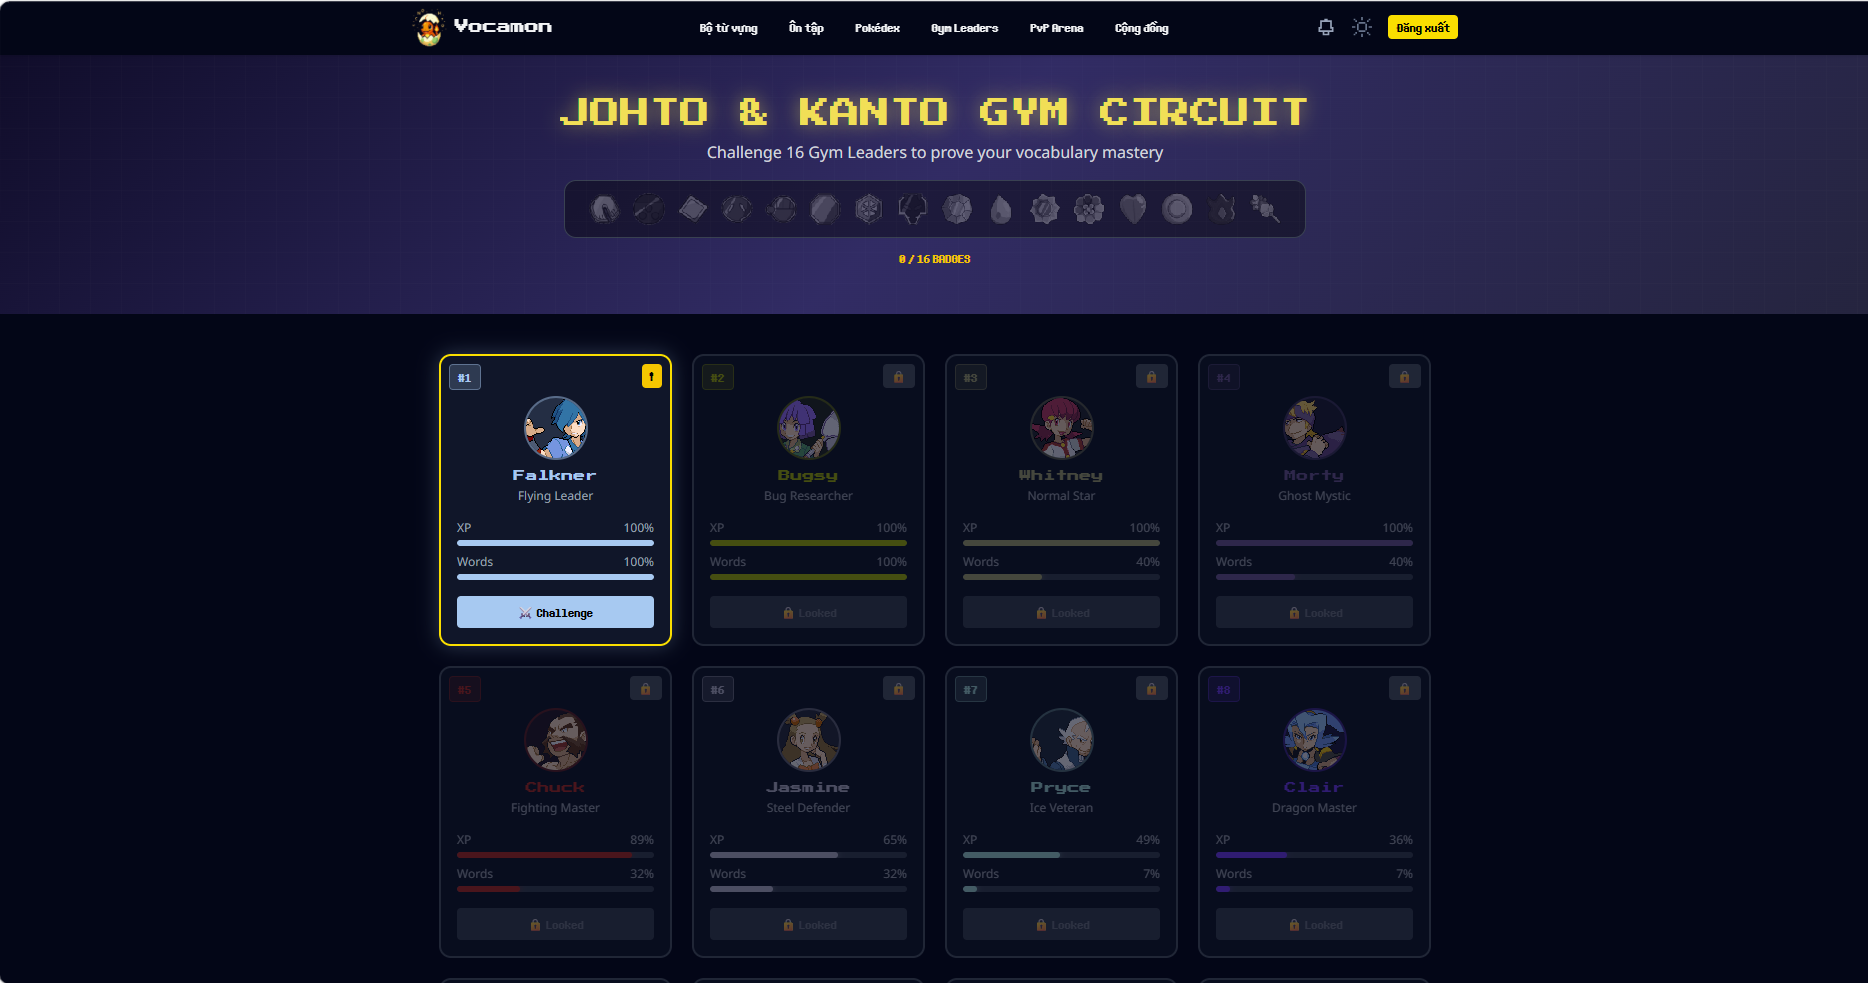
\includegraphics[width=15cm]{images/Final_PvEllobby.png}
\caption{Màn hình danh sách đối thủ PvE.}
\label{fig_battle_PvE}
\end{figure}

\begin{figure}[H]
\centering
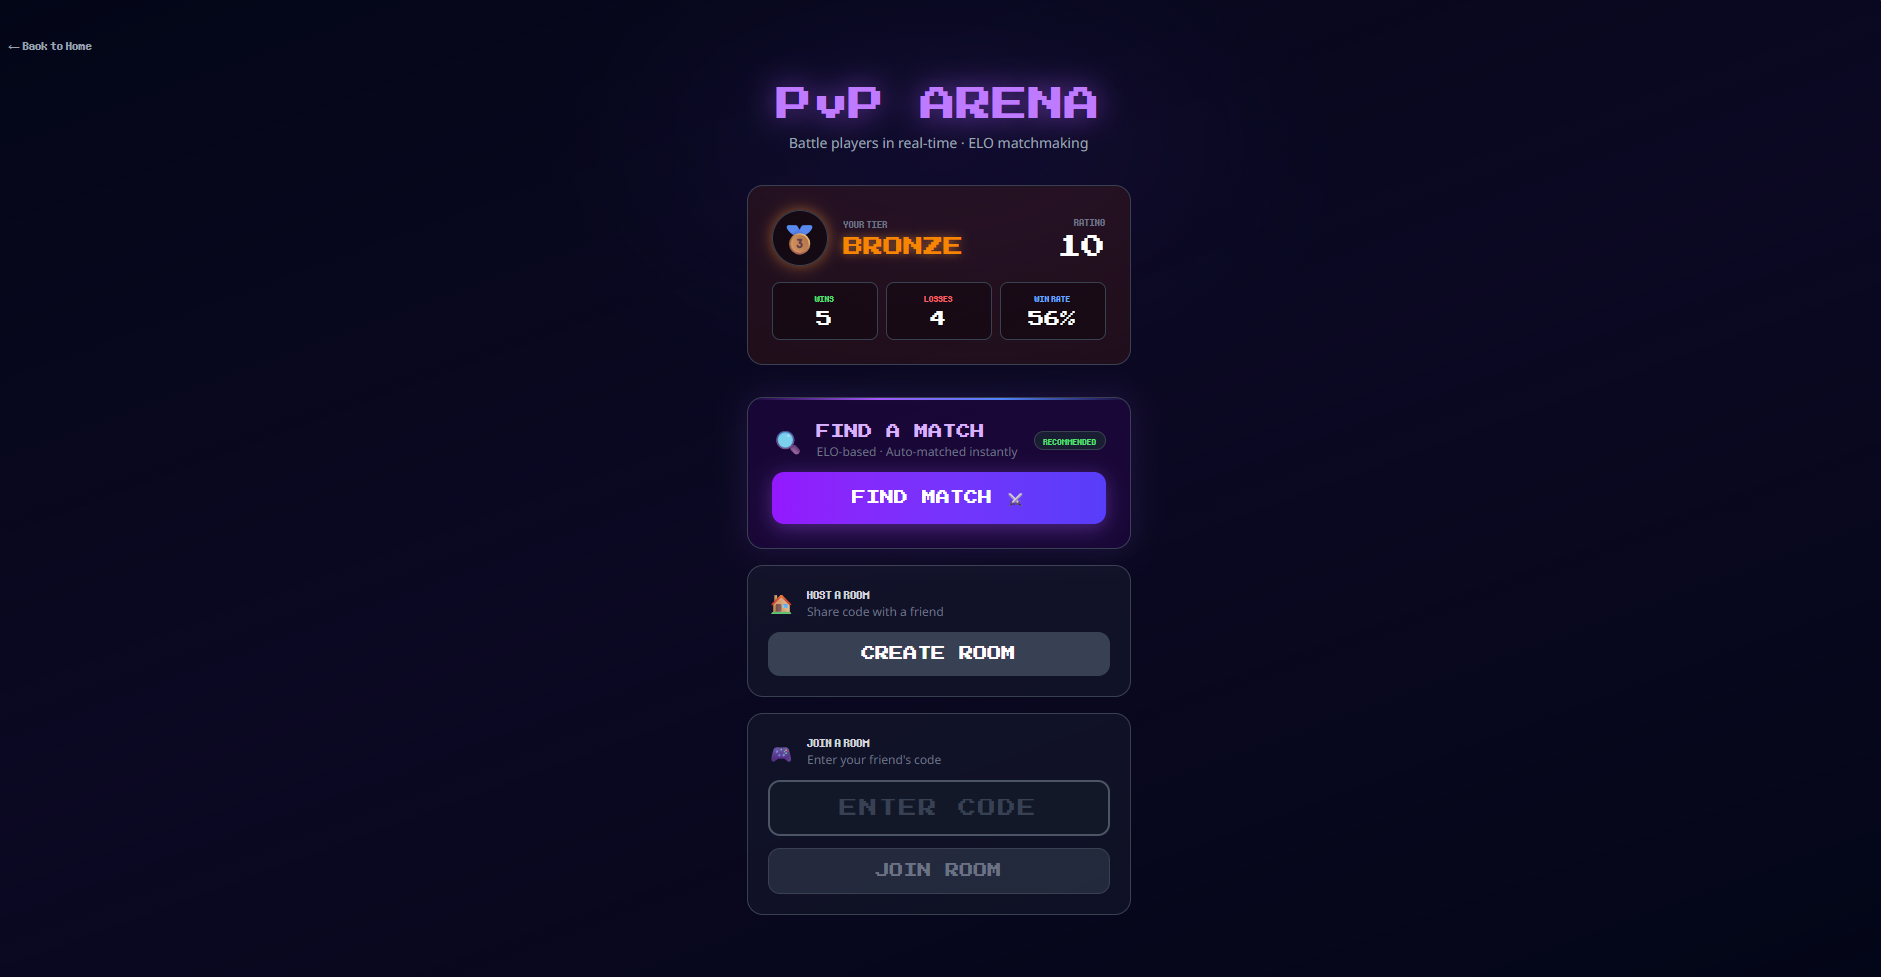
\includegraphics[width=15cm]{images/Final_Pvp_lobby.png}
\caption{Màn hình sảnh chờ PvP.}
\label{fig_battle_PvP}
\end{figure}

\subsection{Bảng điều phối quản trị viên}

Song song với ứng dụng học tập dành cho người dùng đầu cuối, hệ thống triển khai một ứng dụng quản trị độc lập hoạt động như một giao diện điều hành tập trung cho đội ngũ vận hành. Việc tách biệt ứng dụng quản trị khỏi ứng dụng học tập không chỉ giảm thiểu bề mặt tấn công mà còn cho phép triển khai độc lập và thiết lập chính sách bảo mật riêng biệt theo từng ứng dụng.

Quy trình xác thực được thực thi theo hai tầng. Tại tầng máy chủ (Backend), AdminController và các controller quản trị liên quan được bảo vệ bởi thuộc tính [Authorize(Roles = "Admin,SuperAdmin")]. Tại tầng giao diện (Frontend), AuthContext đọc JWT được lưu trong Cookie của trình duyệt, giải mã claim vai trò và kiểm tra ngay tại khởi động ứng dụng — bất kỳ token nào không mang vai trò \textbf{Admin} hoặc \textbf{SuperAdmin} sẽ bị xóa Cookie và chuyển hướng về trang đăng nhập. Để duy trì phiên làm việc không gián đoạn, luồng làm mới token (Refresh Token Rotation) được tích hợp trực tiếp vào Axios interceptor: khi nhận phản hồi HTTP 401, hệ thống tự động gọi endpoint /auth/refresh-token, cập nhật Access Token mới và thực hiện lại yêu cầu gốc mà không yêu cầu quản trị viên đăng nhập lại.

Giao diện điều hướng của ứng dụng được thiết kế theo nguyên tắc hiển thị điều kiện dựa trên vai trò. Thanh bên chia thành bốn nhóm mục điều hướng. Hai nhóm đầu hiển thị với mọi quản trị viên: nhóm User Management gồm ba mục (Danh sách người dùng, Phân quyền vai trò, Nhóm người dùng) và nhóm Content gồm sáu mục (Kho từ vựng, Từ điển, Nhiệm vụ \& Thành tích, Vận hành Gym, Thú ảo, Vật phẩm). Hai nhóm cuối chỉ xuất hiện với tài khoản \textbf{SuperAdmin}: nhóm System gồm bốn mục giám sát (Phát sóng thông báo, Bảng xếp hạng PvP, Xem lại trận đấu, Phân tích phiên học) và nhóm Settings gồm bốn mục vận hành hạ tầng (System Health, System Config, Nhật ký hoạt động, Cài đặt chung). Trang \textbf{System Config} trình bày các tham số chia thành hai danh mục: SRS (các hằng số SM-2) và GAME\_BALANCE (cân bằng trò chơi), với cảnh báo rõ ràng rằng thay đổi có hiệu lực ngay lập tức trên toàn hệ thống; trang \textbf{Gym Operations} cho phép chỉnh sửa BotAccuracy và BotAvgResponseMs cho từng Gym Leader.

\begin{figure}[H]
\centering
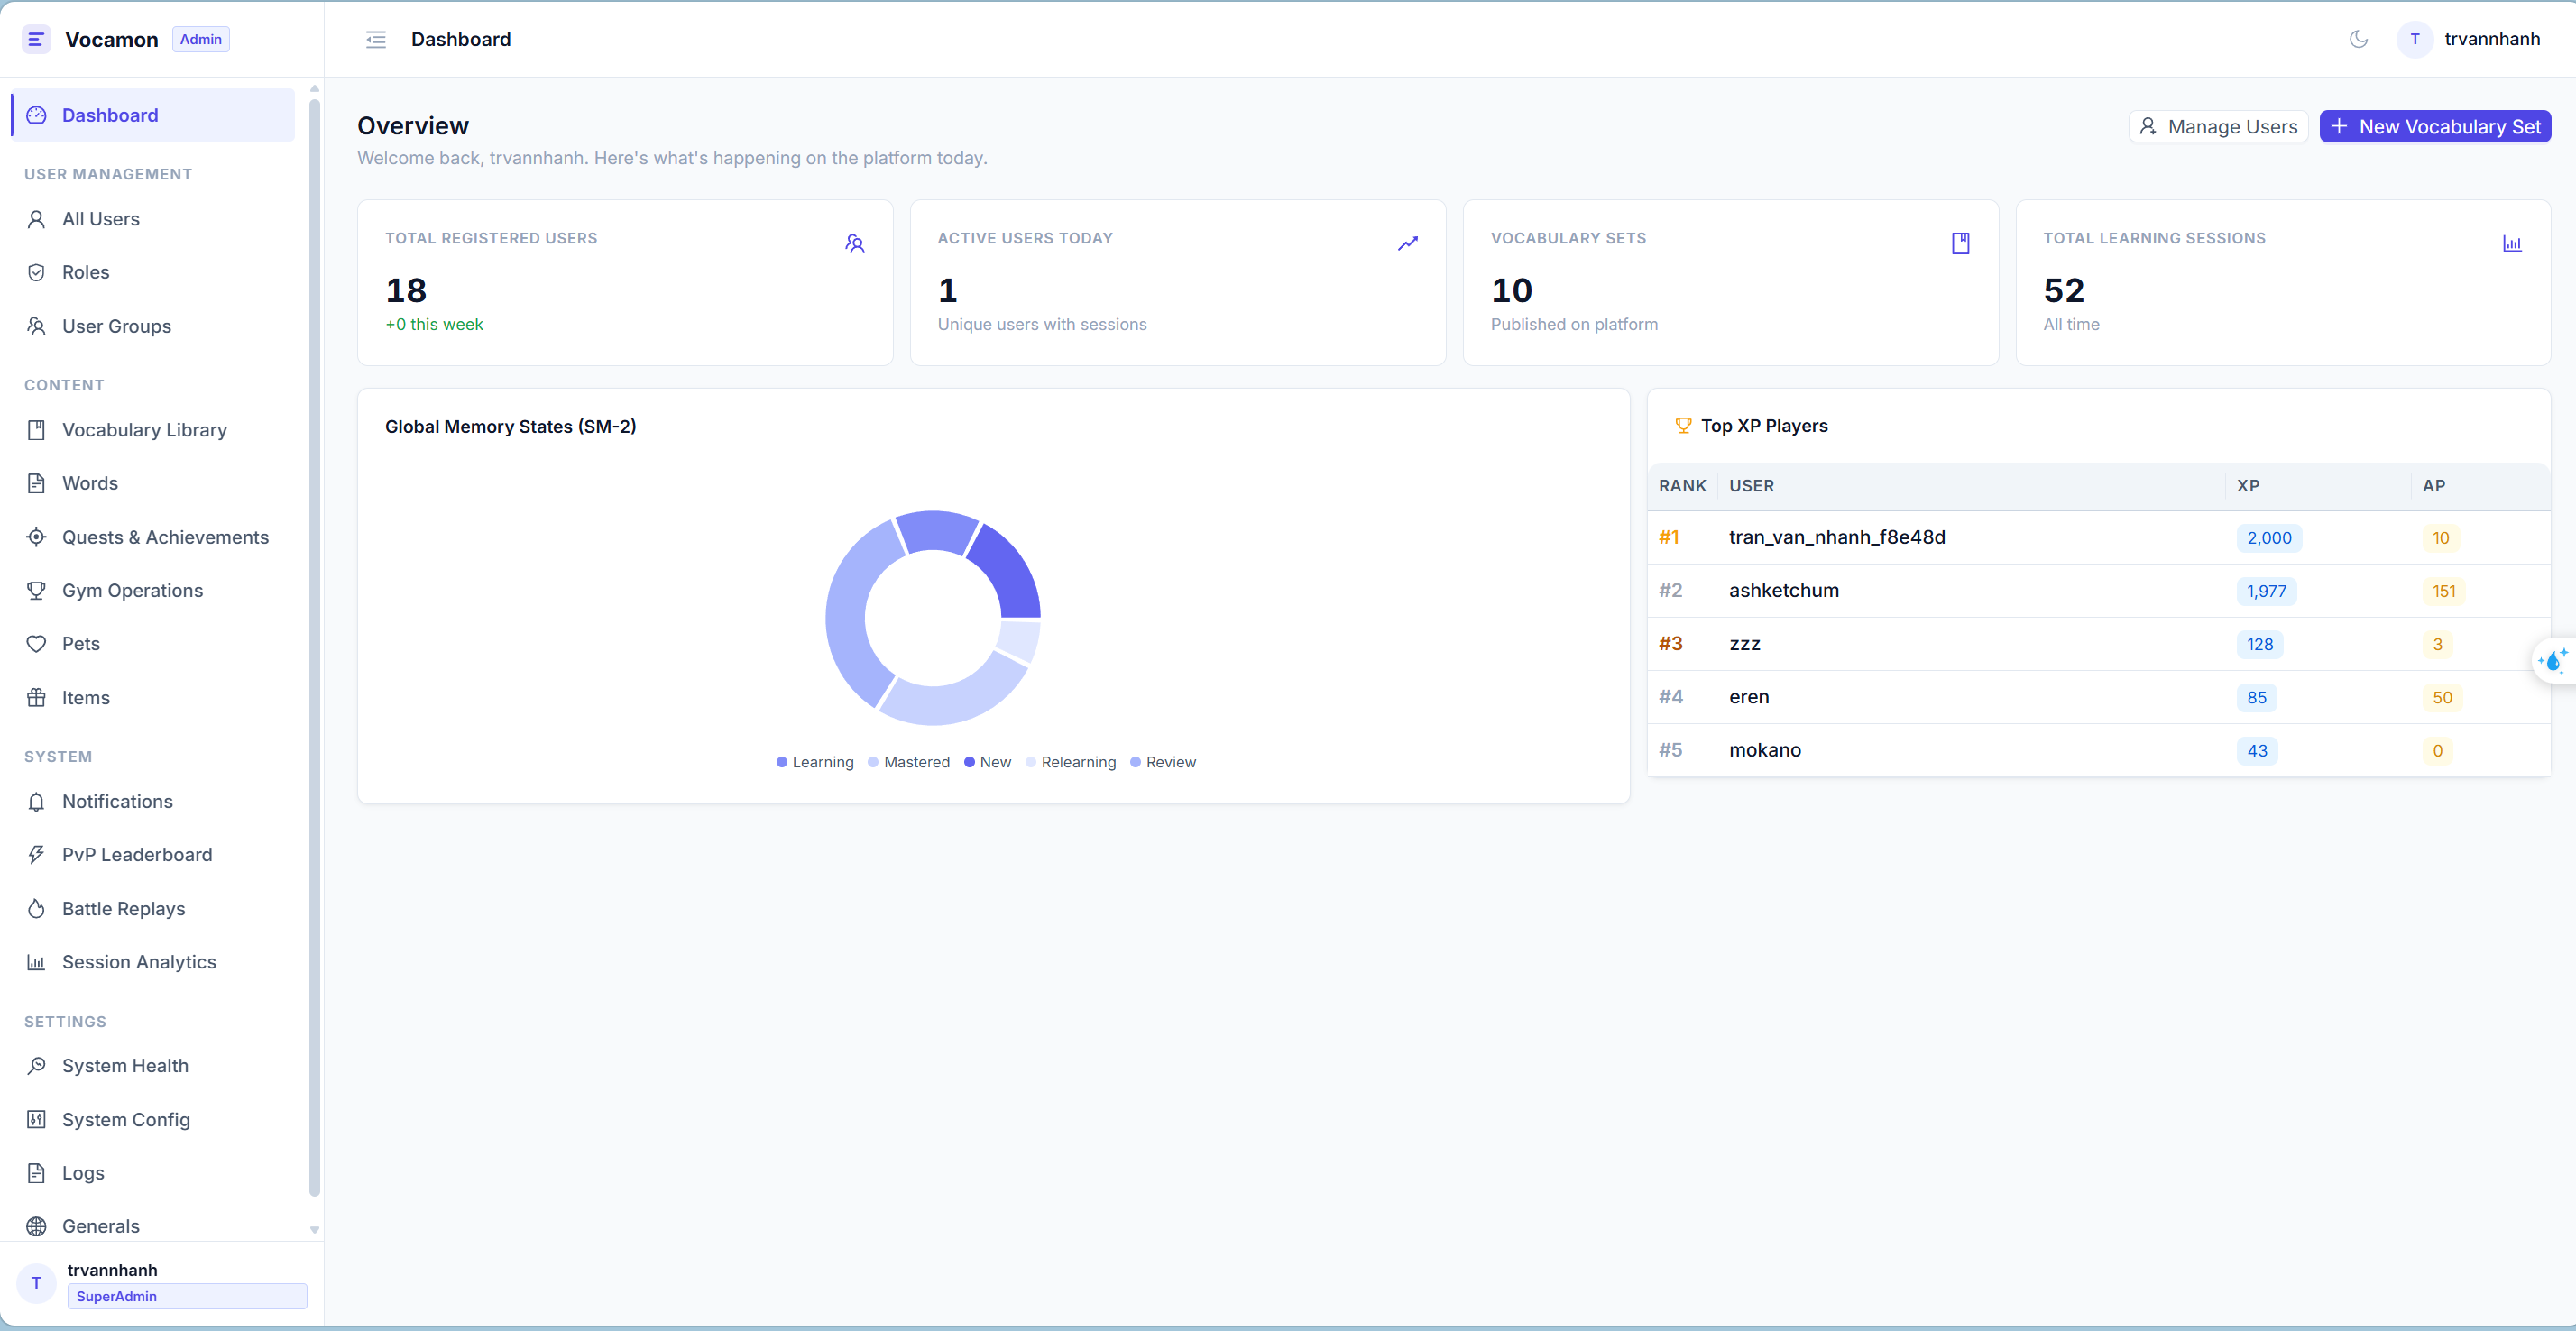
\includegraphics[width=15cm]{images/IF_Admin.png}
\caption{Giao diện bảng điều phối quản trị viên.}
\label{fig:ch3_admin}
\end{figure}

Nhờ sự phối hợp giữa kiểm soát truy cập tầng API và lớp điều hướng phía giao diện, hệ thống đảm bảo rằng quyền hạn của từng vai trò được thực thi nhất quán ở cả hai phía — ngay cả khi quản trị viên cố tình truy cập trực tiếp URL bị hạn chế, yêu cầu tương ứng vẫn sẽ bị Backend từ chối do không đáp ứng điều kiện claim.


\subsection{Tích hợp trí tuệ nhân tạo và tự động hóa nội dung học liệu}

Một trong những điểm kỹ thuật nổi bật của hệ thống là khả năng tự động hóa quá trình biên soạn từ vựng thông qua tích hợp đồng thời ba dịch vụ bên ngoài: Google Gemini API, Unsplash API và bộ nhớ đệm Redis phân tán.

Khi quản trị viên nhập danh sách từ vựng thô vào hệ thống, GeminiAiService sẽ gọi Gemini API (mô hình gemini-2.5-flash) để sinh tự động toàn bộ metadata bao gồm phiên âm IPA, nghĩa tiếng Việt, câu ví dụ ngữ cảnh, phân loại từ loại và cấp độ CEFR tương ứng. Nhằm tuân thủ giới hạn tần suất của API, dữ liệu được xử lý theo từng lô (batch) với kích thước mặc định là 10 từ và khoảng dừng 5.000 ms giữa các lô, đảm bảo tính ổn định khi xử lý danh sách từ vựng lớn. Song song với việc sinh metadata, UnsplashService truy vấn Unsplash API để lấy URL hình ảnh minh họa phù hợp theo ngữ nghĩa của từng từ, giúp kích thích khả năng liên tưởng hình ảnh trong quá trình học tập.

Điểm then chốt về hiệu năng trong luồng này là lớp VocabularyAiCacheService, được triển khai dựa trên IDistributedCache — giao diện tiêu chuẩn của ASP.NET Core ánh xạ tới Redis trong môi trường thực tế. Mỗi kết quả AI cho một từ vựng được lưu cache với khóa có tiền tố vocab-ai-preview: và thời gian tồn tại (TTL) là 7 ngày. Chiến lược này cho phép hệ thống bỏ qua hoàn toàn lần gọi Gemini API đối với các từ đã được xử lý trước đó, giảm thiểu chi phí vận hành và độ trễ phản hồi đáng kể. Quan trọng hơn, lớp cache được thiết kế theo nguyên tắc graceful degradation: nếu Redis không khả dụng, luồng xử lý vẫn tiếp tục bình thường bằng cách gọi Gemini API trực tiếp, tránh tình trạng cascading failure.

\begin{figure}[H]
\centering
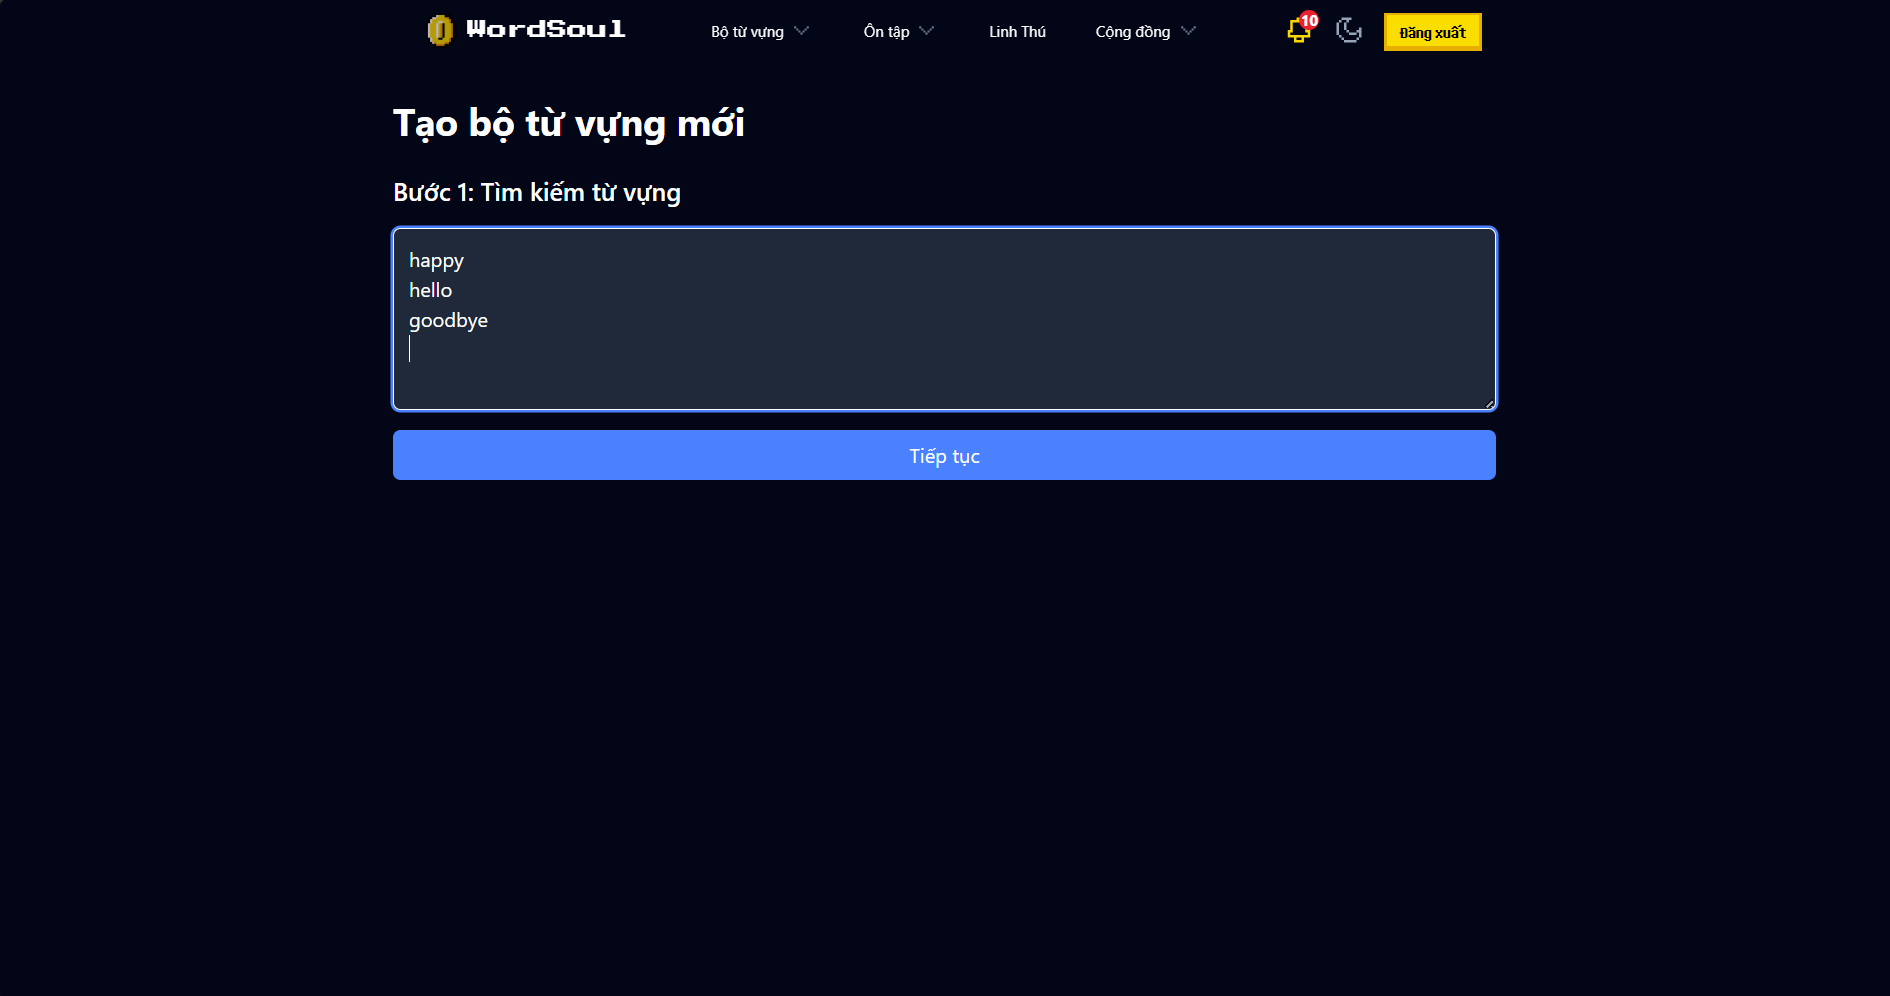
\includegraphics[width=15cm]{images/Final_IF_Set1.png}
\caption{Giao diện sinh metadata từ vựng tự động bằng Gemini AI.}
\label{fig:ch3_ai_generate}
\end{figure}

\subsection{Dịch vụ tổng hợp âm thanh và câu hỏi nghe hiểu}

Nhằm hỗ trợ toàn diện kỹ năng nghe hiểu (Listening) — một trong bốn dạng tương tác cốt lõi của phiên học — hệ thống tích hợp Azure AI Speech SDK để tổng hợp giọng đọc tiếng Anh chuẩn và lưu trữ kết quả trên Azure Blob Storage.

Luồng xử lý được vận hành bởi AzureSpeechService: khi một từ vựng mới được thêm vào hệ thống, phương thức SynthesizeAndUploadAsync gọi Azure Cognitive Services với giọng đọc en-US-AndrewNeural và định dạng đầu ra MP3 (Audio16Khz32KBitRateMonoMp3). Tệp âm thanh sau khi được tổng hợp sẽ được tải lên Azure Blob Storage và URL công khai sẽ được ghi vào trường AudioUrl của bản ghi \textbf{Vocabularies} trong cơ sở dữ liệu. Trong phiên học, khi người dùng gặp câu hỏi dạng Listening, Frontend trực tiếp phát tệp MP3 từ URL Blob Storage — không cần gọi lại API tổng hợp, đảm bảo độ trễ phát âm thanh ở mức tối thiểu.

Sự lựa chọn Azure Blob Storage thay vì các giải pháp lưu trữ nội bộ xuất phát từ hai lý do kỹ thuật chính: thứ nhất, mô hình CDN tích hợp của Azure cho phép phân phối tệp âm thanh tới người dùng với độ trễ thấp bất kể vị trí địa lý; thứ hai, khả năng mở rộng tự động loại bỏ rủi ro về giới hạn dung lượng khi quy mô kho từ vựng tăng trưởng.

\subsection{Hệ thống nhiệm vụ hàng ngày, thành tích và tồn kho vật phẩm}

Bên cạnh vòng lặp học tập chính, hệ thống duy trì hai cơ chế thúc đẩy hành vi dài hạn song song: nhiệm vụ hàng ngày (Daily Quest) và hệ thống thành tích (Achievement).

Mỗi khi người dùng đăng nhập vào ngày mới, DailyQuestService kiểm tra xem nhiệm vụ trong ngày đã được tạo chưa — nếu chưa, hệ thống sẽ sinh ngẫu nhiên một tập hợp nhiệm vụ từ danh sách các mẫu đang kích hoạt và gán cho người dùng. Mỗi nhiệm vụ có loại phần thưởng riêng biệt: XP, vật phẩm hoặc thú ảo. Khi người dùng đạt đủ tiến độ và nhận thưởng, ClaimRewardAsync điều phối luồng xử lý phần thưởng tương ứng thông qua các service chuyên biệt.

Song song với nhiệm vụ ngắn hạn, UserAchievementService theo dõi tiến độ thành tích dài hạn. Phương thức UpdateAchievementProgressAsync được gọi sau mỗi sự kiện nghiệp vụ quan trọng — hoàn thành phiên học, mở khóa thú ảo, đạt chuỗi rèn luyện — nhằm cập nhật ProgressValue cho tất cả thành tích có ConditionType tương ứng. Khi tiến độ vượt ngưỡng, thành tích được đánh dấu hoàn thành và người dùng có thể nhận vật phẩm phần thưởng. Toàn bộ các thao tác cập nhật thành tích được bọc trong giao dịch cơ sở dữ liệu (BeginTransactionAsync) để đảm bảo tính nguyên tử.

Hệ thống tồn kho được bảo vệ khỏi tranh chấp đồng thời (race condition) thông qua cơ chế khóa cấp người dùng trong UserInventoryService: mỗi userId được ánh xạ tới một SemaphoreSlim(1,1) riêng biệt. Điều này đảm bảo rằng khi nhiều yêu cầu thêm/bớt vật phẩm xảy ra đồng thời cho cùng một người dùng — ví dụ hoàn thành nhiệm vụ và nhận thưởng trận đấu trong cùng thời điểm — số lượng tồn kho luôn được cập nhật chính xác mà không cần khóa ở tầng cơ sở dữ liệu.

\subsection{Cơ chế buff từ thú ảo và mô hình cân bằng trò chơi}

Hệ thống đã hiện thực hóa một mô hình cân bằng trò chơi hai tầng: buff thuộc tính từ thú ảo đang kích hoạt và cơ chế leo thang xác suất phần thưởng theo cột mốc.

PetBuffService tính toán các chỉ số buff dựa trên sự giao thoa giữa PetType và PetRarity của thú ảo đang kích hoạt. Mỗi kiểu nguyên tố cung cấp một loại buff đặc thù: ví dụ, hệ Fire tăng hệ số nhân XP, hệ Water tăng xác suất bắt thú ảo, hệ Grass cung cấp lá chắn gợi ý, hệ Electric giảm hình phạt khi trả lời sai. Bên cạnh đó, độ hiếm của thú ảo nhân thêm hệ số khuếch đại vào toàn bộ buff: Common (1.0×), Uncommon (1.2×), Rare (1.4×), Epic (1.7×) và Legendary (2.0×). Nếu thú ảo sở hữu thuộc tính phụ (SecondaryType), các buff sẽ được tổng hợp theo nguyên tắc cộng dồn, tạo ra những tổ hợp sức mạnh độc đáo thúc đẩy chiến lược sưu tầm và lựa chọn thú ảo.

Tầng thứ hai của mô hình cân bằng nằm ở cơ chế phần thưởng thú ảo sau phiên học, được điều phối bởi SetRewardPetService. Thay vì xác suất cố định, hệ thống áp dụng hệ số nhân leo thang tỷ lệ thuận với số lần hoàn thành bộ từ: dưới 5 lần (hệ số 1×), từ 5 đến 10 lần (5×), từ 10 đến 20 lần (10×), từ 20 đến 50 lần (20×) và từ 50 lần trở lên (50×). Điều này có nghĩa là những thú ảo Legendary vốn có xác suất rất thấp sẽ dần trở nên khả dụng hơn đối với những người học kiên trì, tạo ra một vòng lặp động lực dài hạn: nỗ lực học thuật tích lũy không chỉ cải thiện năng lực ngôn ngữ mà còn trực tiếp mở ra các phần thưởng giải trí xứng đáng.

\subsection{Xác thực đa phương thức: tích hợp Google OAuth 2.0}

Bên cạnh luồng đăng nhập truyền thống bằng tên đăng nhập và mật khẩu, hệ thống triển khai xác thực xã hội thông qua GoogleOAuthService nhằm giảm rào cản đăng ký và nâng cao trải nghiệm người dùng. Luồng xử lý tuân thủ chuẩn OAuth 2.0 Authorization Code Flow: Frontend chuyển hướng người dùng tới trang xác nhận của Google kèm theo ClientId và RedirectUri đã đăng ký; sau khi người dùng chấp thuận, Google trả về một Authorization Code ngắn hạn. GoogleOAuthService thực hiện bước exchange: gửi code lên endpoint https://oauth2.googleapis.com/token để nhận Access Token, sau đó dùng token này truy vấn thông tin định danh người dùng.

Kết quả xác thực được xử lý theo hai nhánh tùy thuộc vào trạng thái tài khoản: nếu email chưa tồn tại trong hệ thống, một tài khoản mới được tạo tự động với mật khẩu ngẫu nhiên; nếu đã tồn tại, phiên đăng nhập được liên kết với tài khoản hiện có. Trong cả hai trường hợp, phản hồi cuối cùng trả về cho Client là cặp JWT và Refresh Token tiêu chuẩn — đảm bảo tính nhất quán hoàn toàn với toàn bộ luồng bảo mật của hệ thống. Thiết kế này cho phép người dùng linh hoạt chuyển đổi giữa hai phương thức xác thực mà không cần tạo tài khoản mới.

\subsection{Dịch vụ nền và thông báo ôn tập tự động}

Hệ thống duy trì hai dịch vụ nền chạy song song với luồng xử lý chính, đảm nhiệm các tác vụ bất đồng bộ quan trọng mà không tác động đến hiệu năng của các API endpoint.

MatchmakingWorker thực thi một vòng lặp với chu kỳ 5 giây, chịu trách nhiệm ghép trận PvP tự động dựa trên chỉ số Elo. Mỗi chu kỳ, worker gọi IMatchmakingQueueService.DrainMatches() để lấy danh sách các cặp người chơi đã được ghép từ hàng đợi. Với mỗi cặp tìm được, worker tạo một phiên PvP mới thông qua IArenaBattleService — người chơi thứ nhất đóng vai Challenger, người chơi thứ hai tự động tham gia — và cuối cùng thông báo kết quả ghép trận tới cả hai Client qua IMatchmakingNotifier. Cơ chế tự động này loại bỏ sự phụ thuộc vào việc chia sẻ mã phòng thủ công trong chế độ Random Matchmaking, rút ngắn đáng kể thời gian chờ và cải thiện trải nghiệm cạnh tranh khi lượng người dùng đồng thời cao.

NotificationBackgroundService vận hành theo chu kỳ một giờ, thực hiện truy vấn trực tiếp vào bảng \textbf{UserVocabularyProgresses} để xác định các mục từ có NextReviewTime đã đến hoặc quá hạn. Với mỗi người dùng có ít nhất một từ cần ôn tập, service kiểm tra điều kiện tránh trùng lặp — không gửi quá một thông báo loại Review chưa đọc trong vòng một giờ — trước khi gọi INotificationService.CreateNotificationAsync. Cơ chế này khép kín vòng lặp SRS: hệ thống không chỉ tính toán lịch ôn tập tối ưu theo SM-2, mà còn chủ động nhắc nhở người học đúng thời điểm trí nhớ bắt đầu suy giảm, tối đa hóa hiệu quả củng cố dài hạn.

\subsection{Kiểm thử đơn vị các thành phần nghiệp vụ}

Nhằm đảm bảo tính đúng đắn của các logic nghiệp vụ cốt lõi và phát hiện sớm các lỗi hồi quy (regression bug) trong suốt vòng đời phát triển, hệ thống áp dụng chiến lược kiểm thử đơn vị (Unit Testing) toàn diện trên nền tảng framework \textbf{xUnit.net}. Bên cạnh đó, thư viện \textbf{Moq} được sử dụng để giả lập (mock) các phụ thuộc ngoại vi như kho lưu trữ dữ liệu và đơn vị làm việc (Unit of Work), trong khi \textbf{FluentAssertions} cung cấp cú pháp kiểm chứng (assertion) gần với ngôn ngữ tự nhiên, giúp tăng tính đọc hiểu của bộ kiểm thử.

Chiến lược kiểm thử tuân thủ nguyên tắc cô lập nghiệp vụ theo từng tầng. Mỗi lớp Service được kiểm thử hoàn toàn độc lập với cơ sở hạ tầng thực tế: toàn bộ các phụ thuộc bao gồm IRepository, IUnitOfWork và các dịch vụ ngoại vi đều được thay thế bằng đối tượng giả lập với hành vi xác định trước. Phương thức khởi tạo CreateService() được triển khai như một hàm trợ giúp (factory helper) trong mỗi lớp kiểm thử, trả về bộ đôi (service, deps) chứa cả đối tượng dịch vụ cần kiểm thử và tập hợp các mock phụ thuộc tương ứng, cho phép từng test case thiết lập kỳ vọng (expectation) một cách tường minh và kiểm soát đầy đủ luồng thực thi. Đối với các nghiệp vụ phụ thuộc vào thời gian thực như lập lịch ôn tập SRS, giao diện ITimeProvider được tiêm vào dịch vụ với một cài đặt cố định (fixed time), đảm bảo mọi phép tính ngày giờ đều cho kết quả tất định (deterministic) và lặp lại được.

Toàn bộ bộ kiểm thử bao gồm \textbf{231 test case} tổ chức thành 15 lớp kiểm thử, phân bố theo sáu nhóm nghiệp vụ chức năng như trình bày tại Bảng~\ref{tab:unit_test_distribution}.

\begin{table}[H]
\centering
\caption{Phân bố bộ kiểm thử đơn vị theo nhóm nghiệp vụ.}
\label{tab:unit_test_distribution}
\renewcommand{\arraystretch}{1.25}
\begin{tabular}{|l|l|c|}
\hline
\textbf{Nhóm nghiệp vụ} & \textbf{Lớp kiểm thử} & \textbf{Số test case} \\
\hline
\multirow{2}{*}{Thuật toán ghi nhớ} & SRSAlgorithmTests & 36 \\
\cline{2-3}
 & SRSServiceTests & 17 \\
\hline
\multirow{4}{*}{Học tập và từ vựng} & LearningSessionServiceTests & 24 \\
\cline{2-3}
 & VocabularySetServiceTests & 28 \\
\cline{2-3}
 & VocabularyServiceTests & 13 \\
\cline{2-3}
 & UserVocabularySetServiceTests & 10 \\
\hline
Xác thực và bảo mật & AuthServiceTests & 16 \\
\hline
\multirow{6}{*}{Gamification} & PetBuffServiceTests & 21 \\
\cline{2-3}
 & SetRewardPetServiceTests & 21 \\
\cline{2-3}
 & UserOwnedPetServiceTests & 16 \\
\cline{2-3}
 & DailyQuestServiceTests & 5 \\
\cline{2-3}
 & UserAchievementServiceTests & 5 \\
\cline{2-3}
 & UserInventoryServiceTests & 5 \\
\hline
Thông báo hệ thống & NotificationServiceTests & 11 \\
\hline
Kiểm thử hiệu năng & ActivityLogServicePerformanceTests & 3 \\
\hline
\multicolumn{2}{|r|}{\textbf{Tổng cộng}} & \textbf{231} \\
\hline
\end{tabular}
\end{table}

Một số kỹ thuật kiểm thử đặc biệt được áp dụng nhằm tăng cường độ phủ và độ chính xác của bộ kiểm thử. Đối với lớp SRSAlgorithmTests, toàn bộ 36 test case được thiết kế như các bài kiểm thử thuần túy (pure unit tests) không sử dụng bất kỳ đối tượng giả lập nào, vì thuật toán SM-2 là một lớp tính toán thuần túy không có phụ thuộc ngoại vi. Các trường hợp biên được kiểm thử bao gồm: ngưỡng sàn hệ số dễ (EF floor tại 1.3), ngưỡng trần (EF ceiling tại 2.5), công thức khoảng cách lặp lại $I(n) = \lceil I(n-1) \times EF \rceil$, cũng như ranh giới hành vi tại điểm đánh giá 2 (lặp lại từ đầu) và điểm 3 (tiếp tục chuỗi ôn tập). Kỹ thuật kiểm thử có tham số (parameterized testing) được thực hiện thông qua thuộc tính [Theory] kết hợp [InlineData], cho phép một test case duy nhất kiểm chứng đồng thời nhiều kịch bản đầu vào--đầu ra mà không lặp lại mã nguồn kiểm thử.

Đối với nhóm gamification, lớp PetBuffServiceTests kiểm thử công thức tính chỉ số buff theo loài (type multiplier), độ hiếm (rarity factor) và loại XP nhận được (XP type), đảm bảo mọi tổ hợp thuộc tính thú ảo đều cho kết quả nhất quán. Lớp SetRewardPetServiceTests xác nhận rằng cơ chế chọn ngẫu nhiên có trọng số (weighted random selection) cho phần thưởng thú ảo phân bố xác suất đúng theo cấu hình độ hiếm, đồng thời kiểm tra các ngưỡng điểm số cột mốc (milestone threshold) kích hoạt phần thưởng. Lớp DailyQuestServiceTests sử dụng DbContext trong bộ nhớ (in-memory) thay vì mock để kiểm tra tính an toàn luồng (thread safety) trong quá trình cập nhật tiến độ nhiệm vụ đồng thời, đảm bảo không xảy ra hiện tượng mất cập nhật (lost update).

Kết quả thực thi bộ kiểm thử đơn vị đạt \textbf{231/231 test case thành công}, với thời gian thực thi toàn bộ bộ kiểm thử dưới 10 giây. Toàn bộ các luồng nghiệp vụ chính bao gồm tính toán lịch ôn tập, quản lý phiên học, xác thực người dùng, hệ thống thú ảo và thông báo đều được xác nhận hoạt động đúng theo đặc tả, tạo nền tảng vững chắc cho việc phát triển và bảo trì hệ thống trong tương lai.

\subsection{Đánh giá tổng thể hiệu năng}

Sau giai đoạn triển khai thực nghiệm, hệ thống đã trải qua quy trình kiểm thử hiệu năng (Load Testing) nghiêm ngặt bằng công cụ k6 nhằm đánh giá sự ổn định của nền tảng trong môi trường vận hành thực tế. Thử nghiệm được thiết lập với kịch bản mô phỏng 100 người dùng ảo truy cập đồng thời trong thời gian 5 phút, tập trung vào điểm cuối API trọng tâm là quy trình xử lý phản hồi câu hỏi ôn tập.

Kết quả đo lường thực tế cho thấy hệ thống đạt được hiệu suất vận hành ấn tượng với thời gian phản hồi ở phân vị thứ 95 (P95) duy trì ổn định tại mức 520 ms. Với lưu lượng xử lý trung bình đạt 58,87 yêu cầu mỗi giây và tổng số 18.742 lượt tương tác được thực hiện thành công, Kết quả kiểm thử xác nhận hiệu năng ổn định của endpoint xử lý câu trả lời (SubmitAnswer) dưới tải tổng hợp 100 người dùng đồng thời trong 5 phút. Cần lưu ý rằng đây là kịch bản kiểm thử giới hạn, chưa bao gồm các điểm nghẽn tiềm ẩn như kết nối SignalR thời gian thực dưới tải cao hay các endpoint gọi đồng thời Gemini API và Azure Speech. Kết quả đạt được khẳng định tính ổn định của luồng nghiệp vụ học tập cốt lõi, đồng thời thiết lập cơ sở kỹ thuật cho các giai đoạn kiểm thử toàn diện hơn trong tương lai.

Về khía cạnh độ tin cậy, hệ thống ghi nhận tỷ lệ lỗi cực thấp ở mức 0,46\%, chủ yếu phát sinh do độ trễ mạng nhất thời trong giai đoạn khởi động tải, trong khi tỷ lệ thất bại của các yêu cầu HTTP và lỗi xác thực đăng nhập đều duy trì ở mức tuyệt đối 0,00\%. Mọi tương tác liên quan đến thuật toán lặp lại ngắt quãng và biến động chỉ số thú ảo đều được thực thi nhất quán tại tầng Backend, loại bỏ hoàn toàn các sai số logic nhờ vào việc áp dụng kiến trúc hành tây (Onion Architecture) kết hợp cùng cơ chế xử lý bất đồng bộ.

Song song đó, qua phản hồi không chính thức từ một số người dùng thử nghiệm trong quá trình phát triển, giao diện hệ thống nhận được đánh giá tích cực về tính trực quan và khả năng sử dụng. Tuy nhiên, đây là thu thập phản hồi phi cấu trúc, chưa thể thay thế cho một đánh giá khả năng sử dụng có hệ thống (usability study). Những kết quả đạt được đã xác nhận tính khả thi kỹ thuật của mô hình nghiên cứu trong việc kết hợp giữa nền tảng công nghệ phần mềm hiện đại và lý thuyết trò chơi hóa vào giáo dục. Thành công này thiết lập một tiền đề kỹ thuật vững chắc cho việc tích hợp các mô hình trí tuệ nhân tạo (AI) để tối ưu hóa lộ trình cá nhân hóa trong tương lai.

\newpage
\begin{figure}[H]
    \centering
    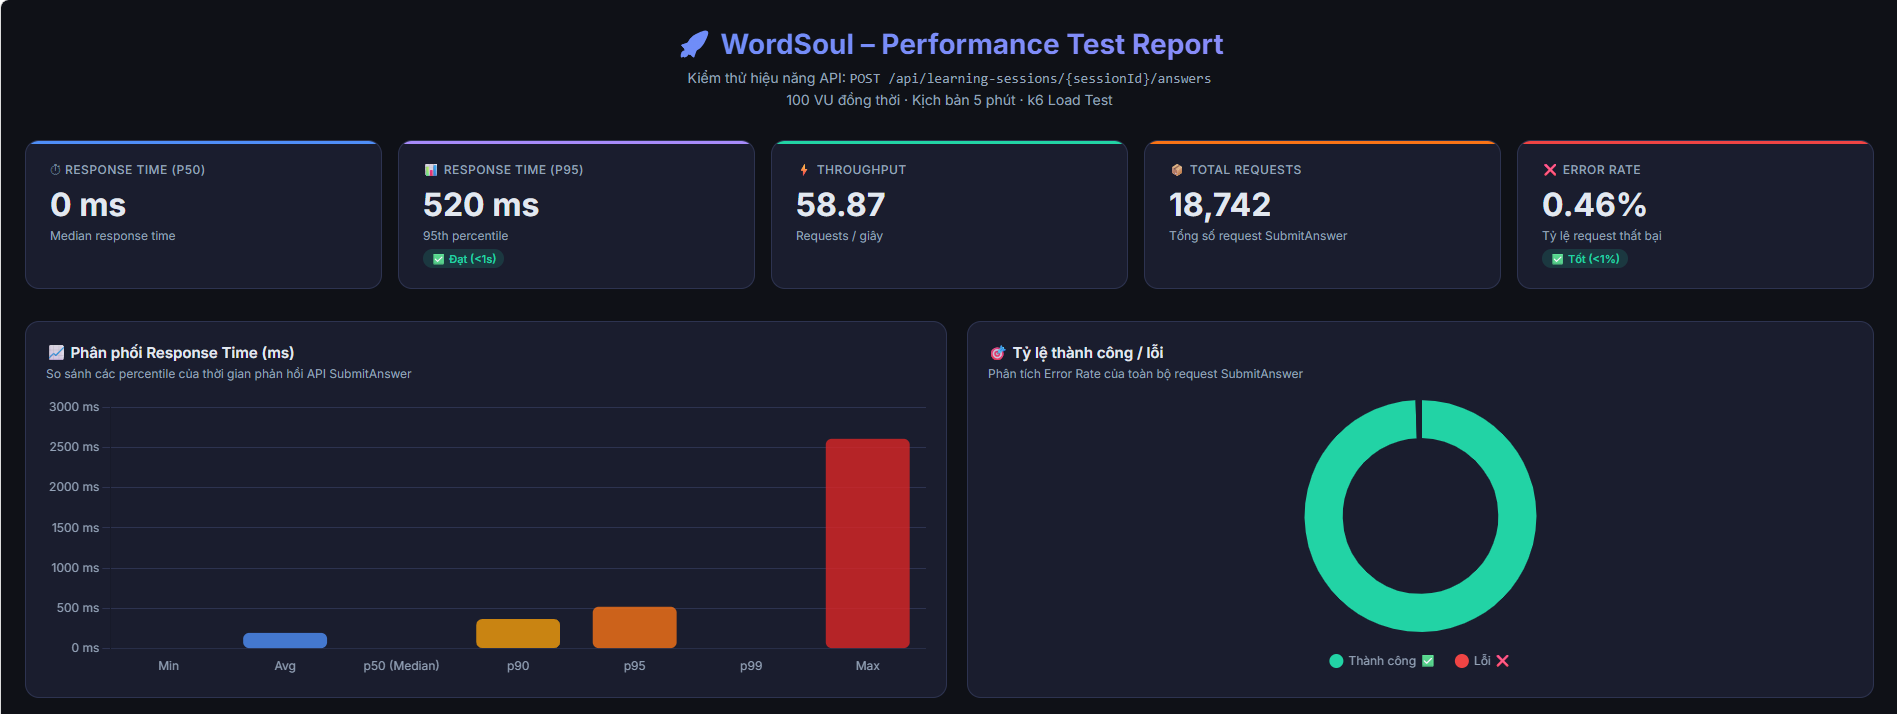
\includegraphics[width=1\textwidth]{images/k6_dashboard_summary.png}
    \caption{Dashboard tổng quan kết quả kiểm thử hiệu năng API SubmitAnswer.}
    \label{fig:k6_summary}
\end{figure}

\begin{figure}[H]
    \centering
    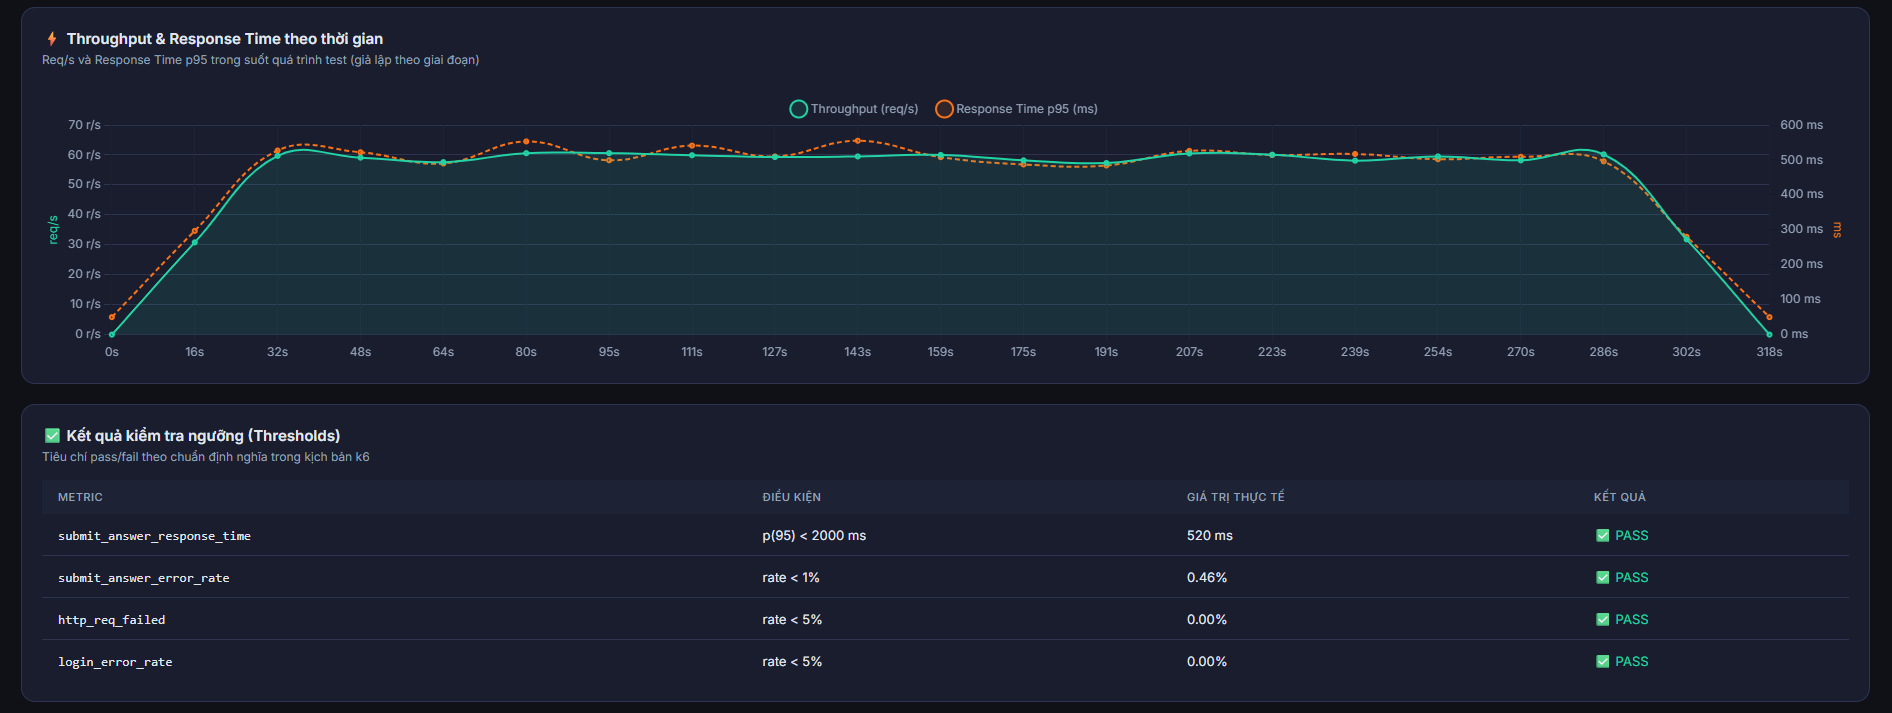
\includegraphics[width=1\textwidth]{images/k6_throughput_graph.png}
    \caption{Biểu đồ biến thiên Throughput và đánh giá các ngưỡng điều kiện (Thresholds).}
    \label{fig:k6_graph}
\end{figure}



\chapter{Kết luận và Hướng phát triển}
\label{Chapter4}

\section{Tổng kết công trình nghiên cứu}

Thông qua quá trình thực hiện, đề tài đã triển khai hệ thống học từ vựng trực tuyến, tích hợp các nguyên lý khoa học nhận thức và cơ chế trò chơi hóa trong một nền tảng web. Về mặt kỹ thuật, hệ thống vận hành ổn định với 231/231 bài kiểm thử đơn vị thành công và thời gian phản hồi P95 đạt 520ms dưới tải 100 người dùng đồng thời. Cần phân biệt rõ rằng các kết quả này chứng minh \textit{tính đúng đắn kỹ thuật} của hệ thống — rằng các tính năng hoạt động đúng theo đặc tả — chứ chưa phải bằng chứng sư phạm về hiệu quả cải thiện ghi nhớ hay duy trì động lực học tập dài hạn. Dự án đã hiện thực hóa một nền tảng có tiềm năng kiểm nghiệm các giả thuyết về Gamification trong giáo dục ngôn ngữ, và việc kiểm nghiệm đó là hướng nghiên cứu cần tiếp nối trong tương lai.

Dưới góc độ chuyên môn, dự án đã hệ thống hóa thành công thuật toán SM-2 để thiết lập một lộ trình ôn tập cá nhân hóa, dựa trên sự phân tích lịch sử phản hồi của từng chủ thể. Việc đa dạng hóa các phương thức tương tác từ Flashcard đến rèn luyện thính giác đã tạo ra một môi trường thực hành truy hồi (Active Recall) đa chiều. Cách tiếp cận này không chỉ giúp củng cố các dấu vết trí nhớ từ nhiều giác quan mà còn gia tăng hiệu quả của việc chuyển dịch thông tin từ trí nhớ ngắn hạn sang lưu trữ dài hạn một cách bền vững.

Điểm thiết kế đặc trưng của Gamification nằm ở việc chuyển dịch trọng tâm từ các áp lực thành tích ngoại cảnh sang cơ chế nuôi dưỡng động lực nội sinh. Thay vì chỉ sử dụng các chỉ số bề nổi, hệ thống đã xây dựng cơ chế gắn kết thông qua thú ảo. Sự phát triển của thú ảo gắn trực tiếp với tiến trình học tập, tạo ra phản hồi tích lũy nhằm đáp ứng nhu cầu về năng lực (Competence) và tự chủ (Autonomy) theo SDT. Việc gắn kết tiến trình tich lũy kiến thức với sự phát triển của thú ảo giúp giảm bớt tính đơn điệu thường gặp trong các công cụ học từ vựng hiện có.

Về phương diện kiến trúc, việc vận hành Onion Architecture trên hệ sinh thái .NET 8 và ReactJS đã đảm bảo cho hệ thống một nền tảng vững chắc và khả năng bảo trì tối ưu. Việc phân tách rạch ròi giữa logic nghiệp vụ cốt lõi và hạ tầng kỹ thuật giúp ứng dụng linh hoạt trước các thay đổi công nghệ. Sự phối hợp của các mẫu thiết kế hiện đại cùng giao thức SignalR đã tạo ra một hạ tầng có độ trễ thấp, sẵn sàng đáp ứng các yêu cầu mở rộng quy mô phục vụ cộng đồng người dùng lớn trong tương lai.

\section{Những hạn chế và rào cản tồn tại}

Mặc dù đạt được những bước tiến quan trọng về kỹ thuật, dự án vẫn còn những khía cạnh cần được nhìn nhận khách quan để cải thiện. Trước hết, cơ chế đối kháng (PvP) hiện tại mới dừng lại ở việc thiết lập các quy tắc logic cơ bản. Việc cân bằng các chỉ số chiến đấu và nâng cấp hiệu ứng hình ảnh để tối ưu hóa trải nghiệm thời gian thực vẫn là một thách thức kỹ thuật lớn, đòi hỏi các giải pháp xử lý băng thông và thuật toán tại Server chuyên sâu hơn.

Bên cạnh đó, khả năng tương thích đa thiết bị vẫn là một giới hạn đáng kể. Các giao diện quản trị chứa mật độ dữ liệu lớn chưa đạt đến độ tối ưu hoàn hảo trên các màn hình di động nhỏ, gây khó khăn cho việc học tập mọi lúc mọi nơi. Đồng thời, do giới hạn về nguồn lực công nghệ tích hợp, hệ thống hiện tại chủ yếu tập trung vào kỹ năng đọc hiểu và ghi nhớ ngữ nghĩa, chưa thể triển khai các phân hệ nhận diện giọng nói (Speech-to-Text) để hỗ trợ toàn diện kỹ năng phát âm và giao tiếp chủ động cho người dùng.

Hạn chế quan trọng nhất của công trình, cần được nhìn nhận thẳng thắn, là sự vắng mặt hoàn toàn của nghiên cứu người dùng (user study) có kiểm soát. Trong khi đề tài đặt ra bài toán nghiên cứu về hiệu quả học tập và động lực dài hạn — dẫn chứng các lý thuyết SDT, đường cong Ebbinghaus và thuật toán SM-2 — toàn bộ kết quả trình bày chỉ xác nhận hệ thống \textit{vận hành đúng theo đặc tả kỹ thuật}, chứ chưa phải bằng chứng rằng hệ thống \textit{cải thiện khả năng ghi nhớ hay duy trì động lực} so với các phương pháp hiện có. Các tuyên bố liên quan đến Gamification — rằng cơ chế thú ảo hỗ trợ SDT hay thúc đẩy sự gắn kết dài hạn — ở giai đoạn này vẫn là giả thuyết thiết kế có căn cứ lý thuyết, chứ chưa phải kết luận được kiểm chứng qua dữ liệu người dùng thực. Để có thể đưa ra những khẳng định mang tính sư phạm, công trình cần được tiếp nối bằng một giai đoạn thực nghiệm có đối chứng, đo lường ít nhất: (1) tỉ lệ duy trì người dùng sau 4--8 tuần so với nhóm đối chứng sử dụng phương pháp học thẻ ghi nhớ thông thường; (2) hiệu quả ghi nhớ dài hạn qua kiểm tra trì hoãn (delayed retention test); (3) mức độ tự báo cáo động lực học tập theo thang đo chuẩn hóa \cite{RyanDeci2017}. Đây là khoảng trống dữ liệu quan trọng nhất cần ưu tiên khắc phục trong các giai đoạn nghiên cứu tiếp theo.

\section{Tầm nhìn và lộ trình hoàn thiện}

Hướng tới mục tiêu chuyển đổi từ một công trình nghiên cứu sang một giải pháp EdTech hoàn chỉnh, lộ trình tương lai sẽ tập trung vào việc chuyên sâu hóa các thành tố Gamification. Việc xây dựng hệ thống kỹ năng đa tầng và chiến thuật đối kháng phức hợp cho thú ảo sẽ biến các phiên học tập thành những trận đấu trí tuệ, đòi hỏi sự kết hợp giữa kiến thức ngôn ngữ và tư duy logic.

Trên phương diện công nghệ, việc ứng dụng Trí tuệ nhân tạo (AI) sẽ là ưu tiên hàng đầu để phân tích sâu sắc hành vi học tập và đặc tính quên lãng của từng cá nhân, từ đó tự động hóa việc kiến tạo lộ trình ôn tập tối ưu. Sự kết hợp của công nghệ xử lý ngôn ngữ tự nhiên (NLP) và nhận diện giọng nói sẽ mở rộng hệ sinh thái sang các kỹ năng nói và phát âm, tạo ra một môi trường rèn luyện ngôn ngữ toàn diện.

Về mặt quy mô cộng đồng, hệ thống định hướng xây dựng một quần thể học thuật bền vững thông qua các tính năng bang hội và sự kiện liên đấu. Để gia tăng tính tiện dụng, việc phát triển ứng dụng di động chính thức trên các nền tảng React Native hoặc Flutter sẽ được triển khai. Toàn bộ hệ thống sẽ được vận hành trên hạ tầng điện toán đám mây chuyên nghiệp với các cơ chế bảo mật và cân bằng tải tự động, nhằm phát triển hệ thống theo hướng tích hợp học tập và yếu tố giải trí.
\chapter{Kết luận}
\label{Chapter5}

% TODO: Nội dung chương 5



% In tài liệu tham khảo
\phantomsection
\addcontentsline{toc}{chapter}{Tài liệu tham khảo}
\printbibheading[title={Tài liệu tham khảo}]
\printbibliography[heading=subbibliography, title={Tiếng Anh}, notkeyword=Tieng, resetnumbers=16] 

% Phần phụ lục
\addcontentsline{toc}{chapter}{Phụ Lục}

\appendix

\chapter{Mã nguồn một số phương thức quan trọng}

Phụ lục này trình bày một số phương thức tiêu biểu trong mã nguồn của hệ thống, được lựa chọn dựa trên mức độ quan trọng trong việc minh họa kiến trúc hệ thống và giải quyết các yêu cầu nghiệp vụ. Các API này không chỉ thực hiện các thao tác CRUD cơ bản mà còn bao hàm các thuật toán xử lý dữ liệu, cơ chế học tập theo \textit{spaced repetition}, cũng như yếu tố \textit{gamification} thông qua hệ thống thú cưng. 

Mục tiêu của phụ lục là cung cấp cho người đọc cái nhìn rõ ràng về cách hiện thực hoá các yêu cầu chức năng, thay vì liệt kê toàn bộ mã nguồn.

\section{API Quản lý Phiên Học}

\textbf{Mục đích:} Khởi tạo, quản lý và hoàn tất các phiên học hoặc ôn tập của người dùng. Đây là điểm vào (entry point) chính để bắt đầu luồng học.

\begin{lstlisting}[language=C, caption={Tạo một phiên học dựa trên bộ từ vựng đã chọn}]
[Authorize(Roles = "User")]
[HttpPost("{vocaSetId}")]
public async Task<IActionResult> CreateLearningSession(int vocaSetId)
{
    var userId = User.GetUserId();
    if (userId == 0) return Unauthorized();
    if (vocaSetId <= 0) return BadRequest("Invalid VocabularySet ID");

    try
    {
        var learningSessionDto = await _learningSessionService.CreateLearningSessionAsync(userId, vocaSetId);
        return Ok(learningSessionDto);
    }
    catch (InvalidOperationException ex)
    {
        _logger.LogWarning(ex, "No unlearned vocabularies found.");
        return NotFound(ex.Message);
    }
}
\end{lstlisting}

API trên thể hiện rõ cách hệ thống:
\begin{itemize}
    \item Xác thực người dùng thông qua JWT và Role.
    \item Kiểm tra quyền sở hữu bộ từ vựng.
    \item Xử lý tình huống không còn từ để học và trả về mã lỗi phù hợp.
\end{itemize}

\section{Thuật Toán Cập Nhật Tiến Trình Học }

\textbf{Mục đích:} Lưu kết quả trả lời và áp dụng cơ chế \textit{spaced repetition} để xác định thời điểm ôn tập tiếp theo.

\begin{lstlisting}[language=C, caption={Cập nhật tiến trình học và tính ngày ôn tập}]
progress.ProficiencyLevel = Math.Min(5, 
    1 + (int)Math.Floor(Math.Log(Math.Max(1, progress.CorrectAttempt), 1.5)));

int daysToAdd = progress.ProficiencyLevel switch
{
    1 => 1,
    2 => 2,
    3 => 4,
    4 => 16,
    _ => 256
};

progress.NextReviewTime = DateTime.UtcNow.AddDays(daysToAdd);
\end{lstlisting}

Đây là phần mang tính học thuật quan trọng, vì nó giúp hệ thống tối ưu tần suất xuất hiện của từ vựng, đảm bảo người học ghi nhớ lâu hơn mà không quá tải.

\section{API Tạo Bộ Từ Vựng }

\textbf{Mục đích:} Tạo bộ từ vựng mới và tự động gán thú cưng phần thưởng theo độ hiếm.

\begin{lstlisting}[language=C, caption={Tự động gán Pet thưởng cho bộ từ vựng}]
var petDistribution = new Dictionary<PetRarity, (int Count, double DropRate)>
{
    { PetRarity.Common, (10, 0.4) },
    { PetRarity.Uncommon, (5, 0.25) },
    { PetRarity.Rare, (3, 0.15) },
    { PetRarity.Epic, (2, 0.05) },
    { PetRarity.Legendary, (1, 0.01) }
};

foreach (var (rarity, (count, dropRate)) in petDistribution)
{
    var pets = await _petRepository.GetRandomPetsByRarityAsync(rarity, count);
    vocabularySet.SetRewardPets.AddRange(pets.Select(pet => new SetRewardPet
    {
        PetId = pet.Id,
        DropRate = dropRate
    }));
}
\end{lstlisting}

Đoạn mã này cho thấy cách hệ thống sử dụng logic xác suất để phân phối phần thưởng, góp phần tăng tính hấp dẫn của quá trình học.

\section{API Nâng Cấp Thú Cưng}

\textbf{Mục đích:} Xử lý logic tăng kinh nghiệm, tăng cấp độ và tiến hoá thú cưng, từ đó gắn kết yếu tố trò chơi vào hệ thống học.

\begin{lstlisting}[language=C, caption={Nâng cấp và tiến hóa thú cưng}]
while (userOwnedPet.Experience >= 100)
{
    userOwnedPet.Level++;
    userOwnedPet.Experience -= 100;
    isLevelUp = true;

    if (currentPet.RequiredLevel != null && 
        userOwnedPet.Level >= currentPet.RequiredLevel &&
        currentPet.NextEvolutionId.HasValue)
    {
        var evolvedPet = await _petRepository.GetPetByIdAsync(currentPet.NextEvolutionId.Value);
        if (evolvedPet != null)
        {
            userOwnedPet.PetId = evolvedPet.Id;
            isEvolve = true;
            break;
        }
    }
}
\end{lstlisting}

API này minh họa cách hệ thống quản lý trạng thái phức tạp của thú cưng, đồng thời đảm bảo tính nhất quán dữ liệu khi người dùng nâng cấp nhiều lần liên tiếp.

\section{Nhận Xét Chung}

Các API trên thể hiện:
\begin{itemize}
    \item Cách hệ thống kết hợp giữa \textbf{xác thực – xử lý nghiệp vụ – lưu trữ dữ liệu}.
    \item Việc áp dụng thuật toán học tập và gamification.
    \item Thiết kế chuẩn RESTful, tách biệt Controller – Service – Repository, dễ mở rộng trong tương lai.
\end{itemize}

Các API CRUD cơ bản khác (xem/xoá/cập nhật Pet, tìm kiếm bộ từ vựng, quản lý người dùng) không được liệt kê ở đây để tránh trùng lặp và giữ tính cô đọng cho phụ lục.


\chapter{Một Số Màn Hình Bổ Sung}

Phụ lục này giới thiệu thêm một số màn hình giao diện của hệ thống , minh hoạ các chức năng phụ trợ như lọc, tìm kiếm, xem chi tiết và điều hướng học tập. Các màn hình này không được mô tả chi tiết trong chương Kết quả đạt được nhưng đóng vai trò quan trọng trong việc nâng cao trải nghiệm người dùng.

\section{Màn hình Danh sách Thú cưng}
\begin{figure}[H]
\centering
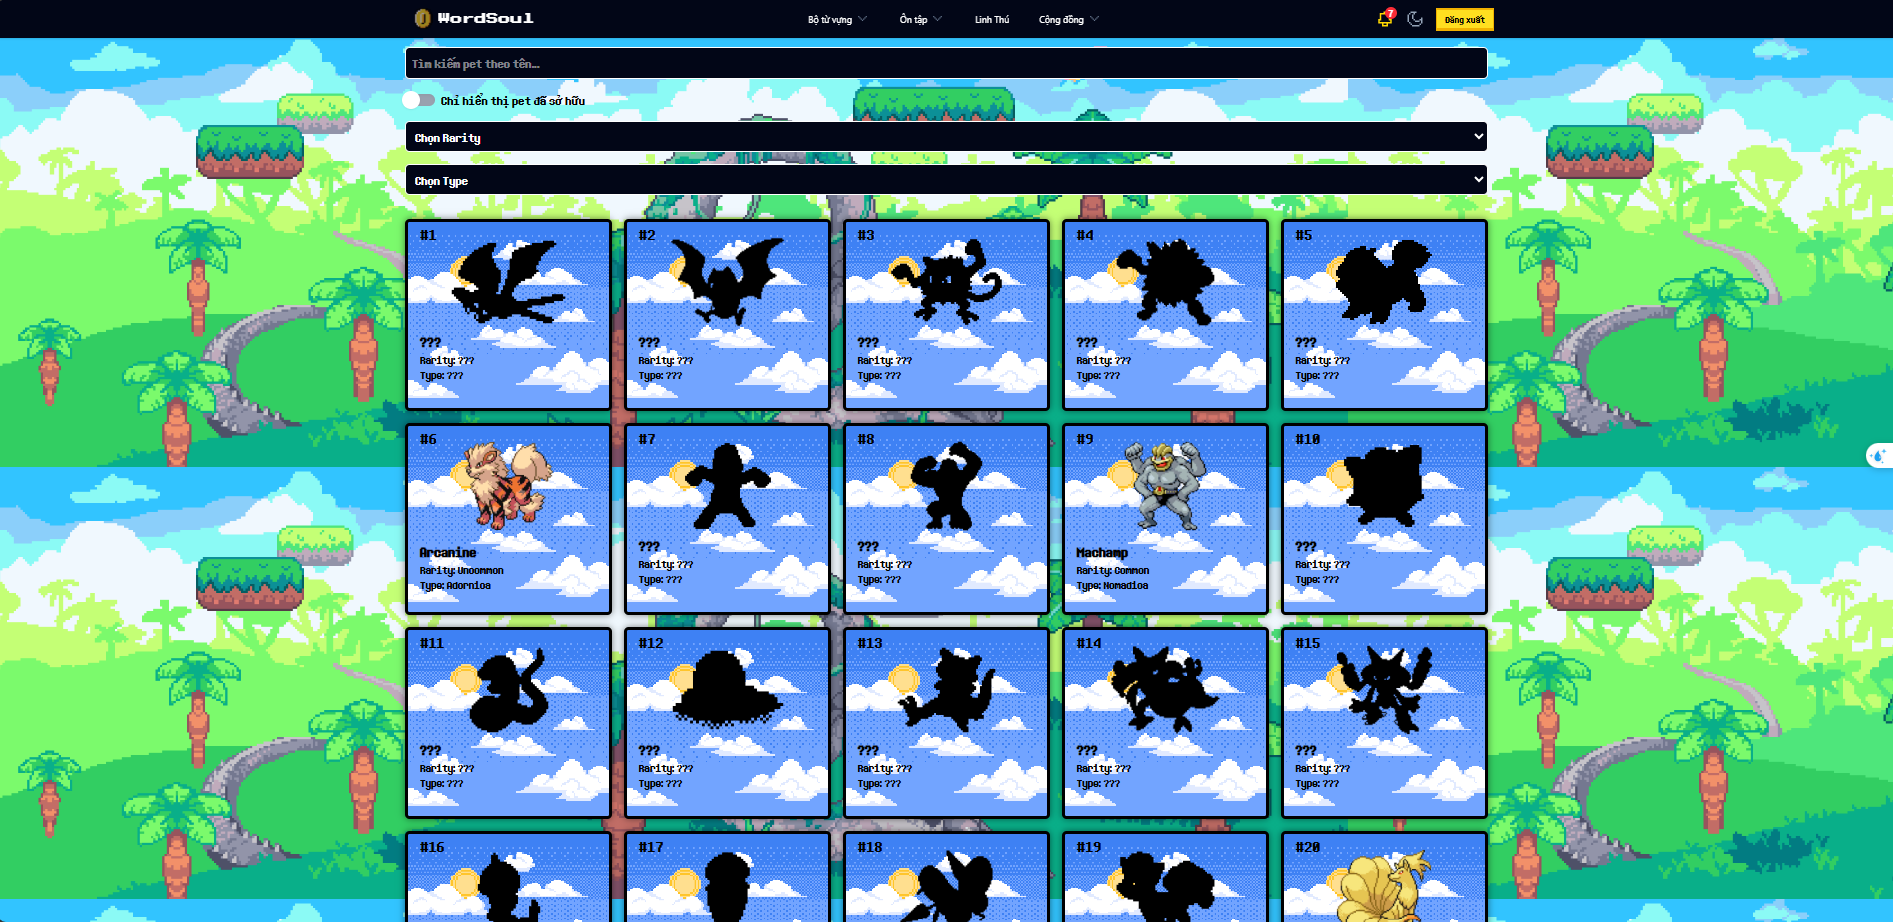
\includegraphics[width=15cm]{images/IF_PetList.png}
\caption{Màn hình danh sách thú cưng với bộ lọc nâng cao.}
\label{fig_pet_list}
\end{figure}

Màn hình này hiển thị toàn bộ thú cưng trong hệ thống và hỗ trợ:
\begin{itemize}
    \item Lọc theo tên thú cưng hoặc chỉ hiển thị thú đã sở hữu.
    \item Lọc theo độ hiếm (\textit{Common, Rare, Epic, Legendary}) và loại (\textit{Beast, Spirit, Machine,...}).
    \item Hiển thị trực quan tình trạng sở hữu, cấp độ hiện tại và tiến trình tiến hoá.
\end{itemize}
Chức năng này giúp người học dễ dàng theo dõi bộ sưu tập, tăng động lực thu thập đầy đủ thú cưng.

\section{Màn hình Chi tiết Bộ từ vựng}
\begin{figure}[H]
\centering
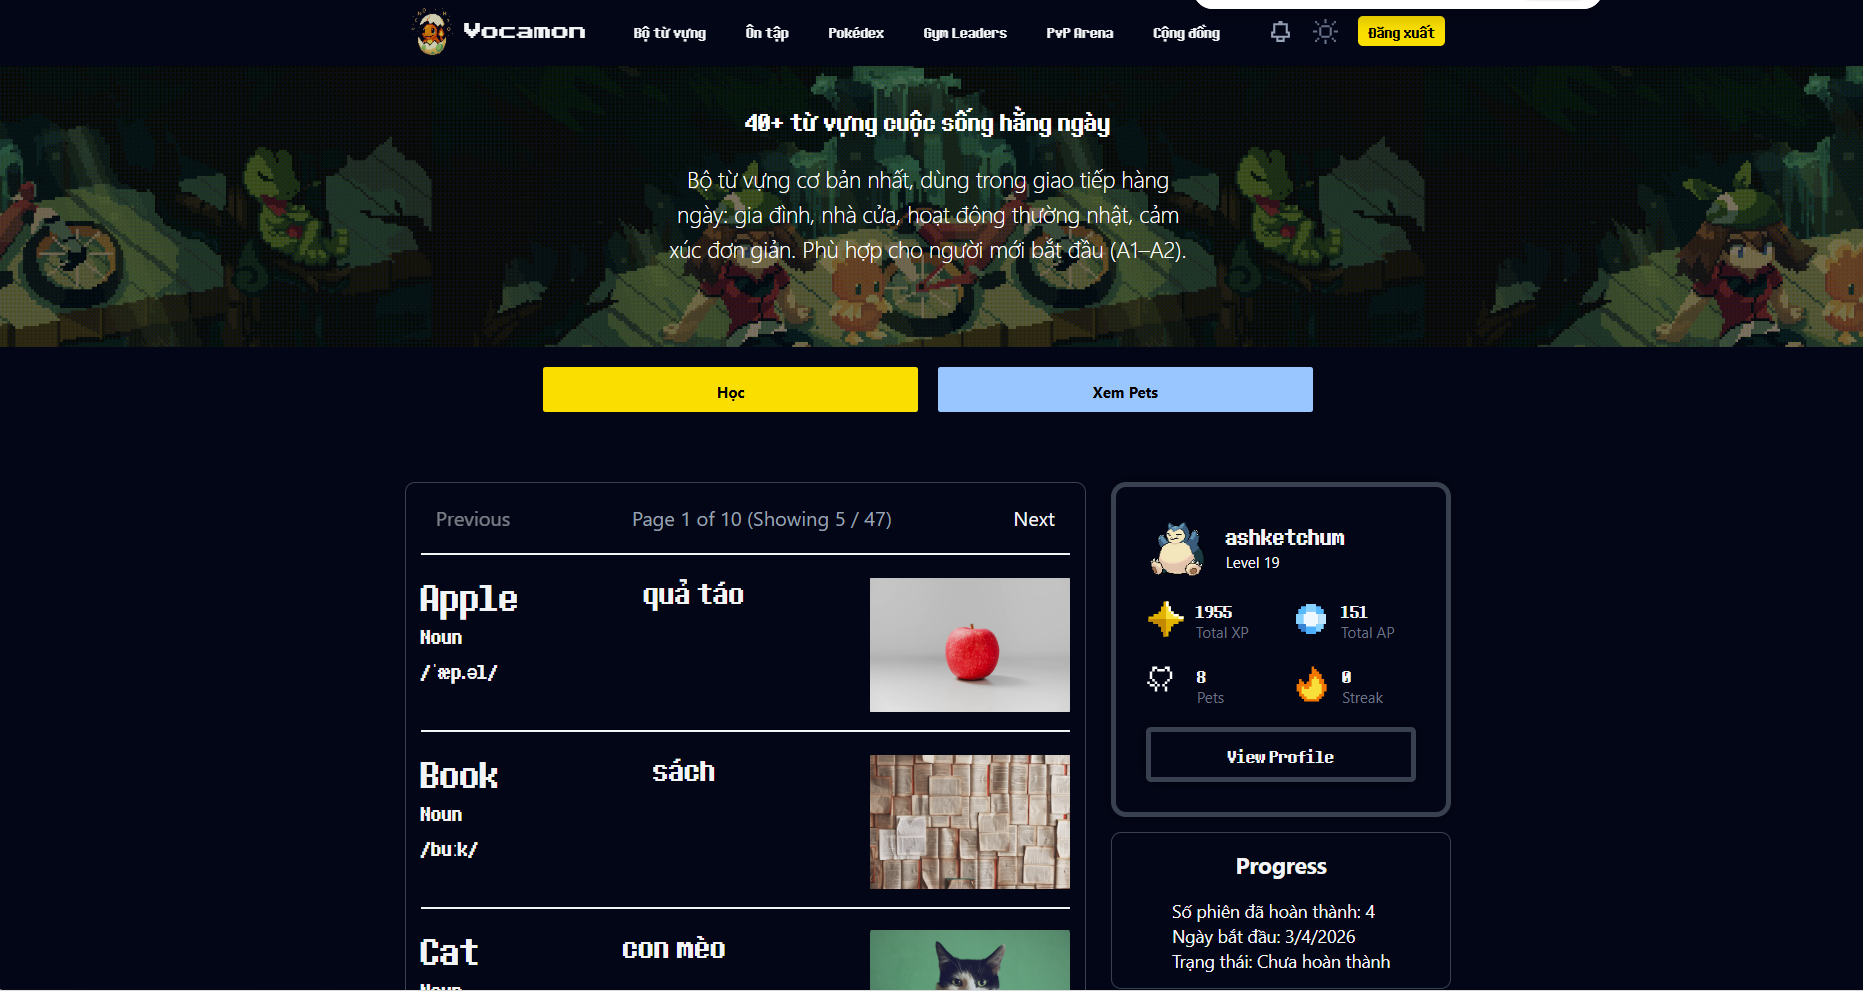
\includegraphics[width=15cm]{images/IF_SetDetail.png}
\caption{Màn hình chi tiết bộ từ vựng.}
\label{fig_set_detail}
\end{figure}

Màn hình này cung cấp thông tin toàn diện về một bộ từ:
\begin{itemize}
    \item Hiển thị tiêu đề, mô tả, ảnh minh họa, chủ đề, độ khó và thú cưng thưởng.
    \item Nút \textbf{Đăng ký bộ từ vựng} (nếu người dùng chưa sở hữu) và nút \textbf{Học} (nếu đã sở hữu).
    \item Nút \textbf{Đã hoàn thành} được disable khi người dùng đã học xong toàn bộ bộ từ.
    \item Danh sách tất cả các từ trong bộ, kèm tiến trình (ví dụ: số lần đúng, mức độ thành thạo).
\end{itemize}
Màn hình này là trung tâm định hướng học tập, giúp người dùng quyết định đăng ký hoặc tiếp tục học.

\section{Màn hình Danh sách Bộ từ vựng}
\begin{figure}[H]
\centering
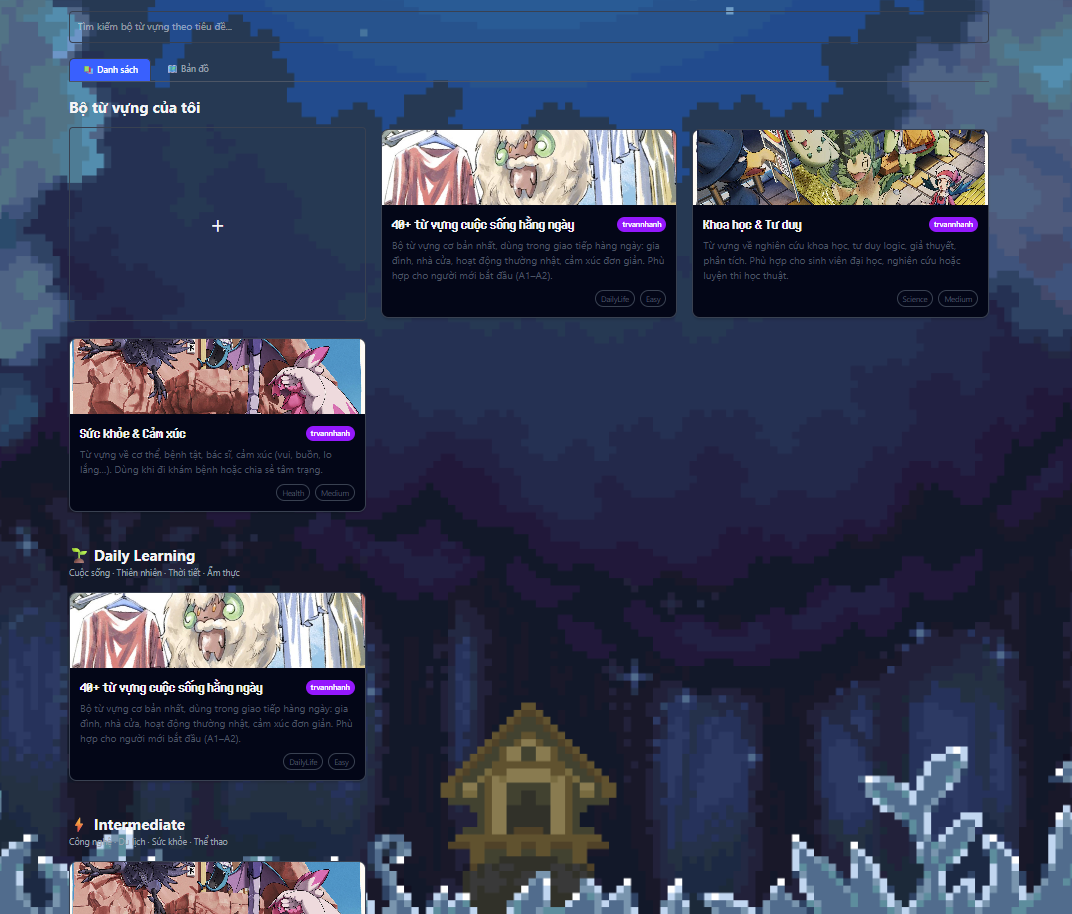
\includegraphics[width=15cm]{images/IF_SetList.png}
\caption{Màn hình danh sách bộ từ vựng.}
\label{fig_set_list}
\end{figure}

Màn hình này cho phép duyệt và tìm kiếm bộ từ vựng:
\begin{itemize}
    \item Lọc theo \textbf{chủ đề} (Theme) và mức độ khó.
    \item Tìm kiếm theo từ khóa để nhanh chóng tìm bộ từ liên quan.
    \item Hiển thị trạng thái sở hữu và số lượng từ còn phải học trong từng bộ.
\end{itemize}

\section{Ý nghĩa và Vai trò}
Các màn hình trong phụ lục này thể hiện sự quan tâm đến \textbf{trải nghiệm người dùng (UX)}:
\begin{itemize}
    \item Tối ưu quá trình điều hướng: người học dễ tìm bộ từ, chọn pet hoặc kiểm tra tiến trình.
    \item Tăng tính cá nhân hóa: hiển thị rõ tình trạng sở hữu, tiến trình học, và khuyến khích hoàn thành.
    \item Hỗ trợ việc mở rộng sau này: thêm bộ lọc nâng cao, sắp xếp theo mức độ phổ biến hoặc ngày tạo.
\end{itemize}
Những màn hình này đóng vai trò quan trọng trong việc biến hệ thống thành một nền tảng học tập có tính cộng đồng và khuyến khích người học quay lại hằng ngày.


\end{document}